
As high-energy physics enters the era of Higgs precision measurement, targeting the $H \rightarrow \gamma \gamma$ decay channel offers a valuable avenue for probing Higgs couplings and production modes. Though its branching ratio is rather small (0.227\% \ref{cite:HiggsBR}), the ATLAS detector's excellent photon reconstruction and energy resolution capabilities provide a very clean avenue for signal and background reconstruction in this channel, leading to high purity compared to other channels.

The Couplings analysis is optimized to measure the cross-sections in a number of STXS regions. While an interpretation using the kappa-framework and EFT methods is currently under development at the time of this writing, the cross-sections in each of the STXS categories are reported as a targeted observable.

The preselection at both object and event level is detailed in Chapters \ref{chap:methods_chapter} and \ref{chap:datamc_chapter}.

\section{Categorization} \label{sec:Categorization} 

A categorization scheme is developed to target the STXS truth bins. The categorization is an improvement over that of the previous $80 fb^{-1}$ Coupling analysis, which sorted events into categories based on a "greedy" sequential approach \ref{cite:couplings80fb}. In the new analysis, which uses the full $139 fb^{-1}$ of data gathered by ATLAS, events are instead sorted into categories based on a unified technique that considers a number of their properties simultaneously to determine the optimal categorization scheme.

Categorization proceeds in two primary steps. First, a multiclassifier Boosted Decision Tree (BDT) is trained to target STXS truth bins. A multiclassifier BDT differs from a binary BDT in that it outputs a vector discriminant corresponding to the probability that an event falls into one of a number of different regions, rather than a binary discriminant simply classifying an event as signal or background. After events are assigned into different classes targeting the STXS truth bins, they are subdivided into categories using a second binary BDT trained in each class, designed to separate Higgs signal from continuum background. The process of the BDT categorization scheme is shown in the cartoon in Figure \ref{fig:global_cat_sketch}.

\begin{figure}[tbp]
  \centering
  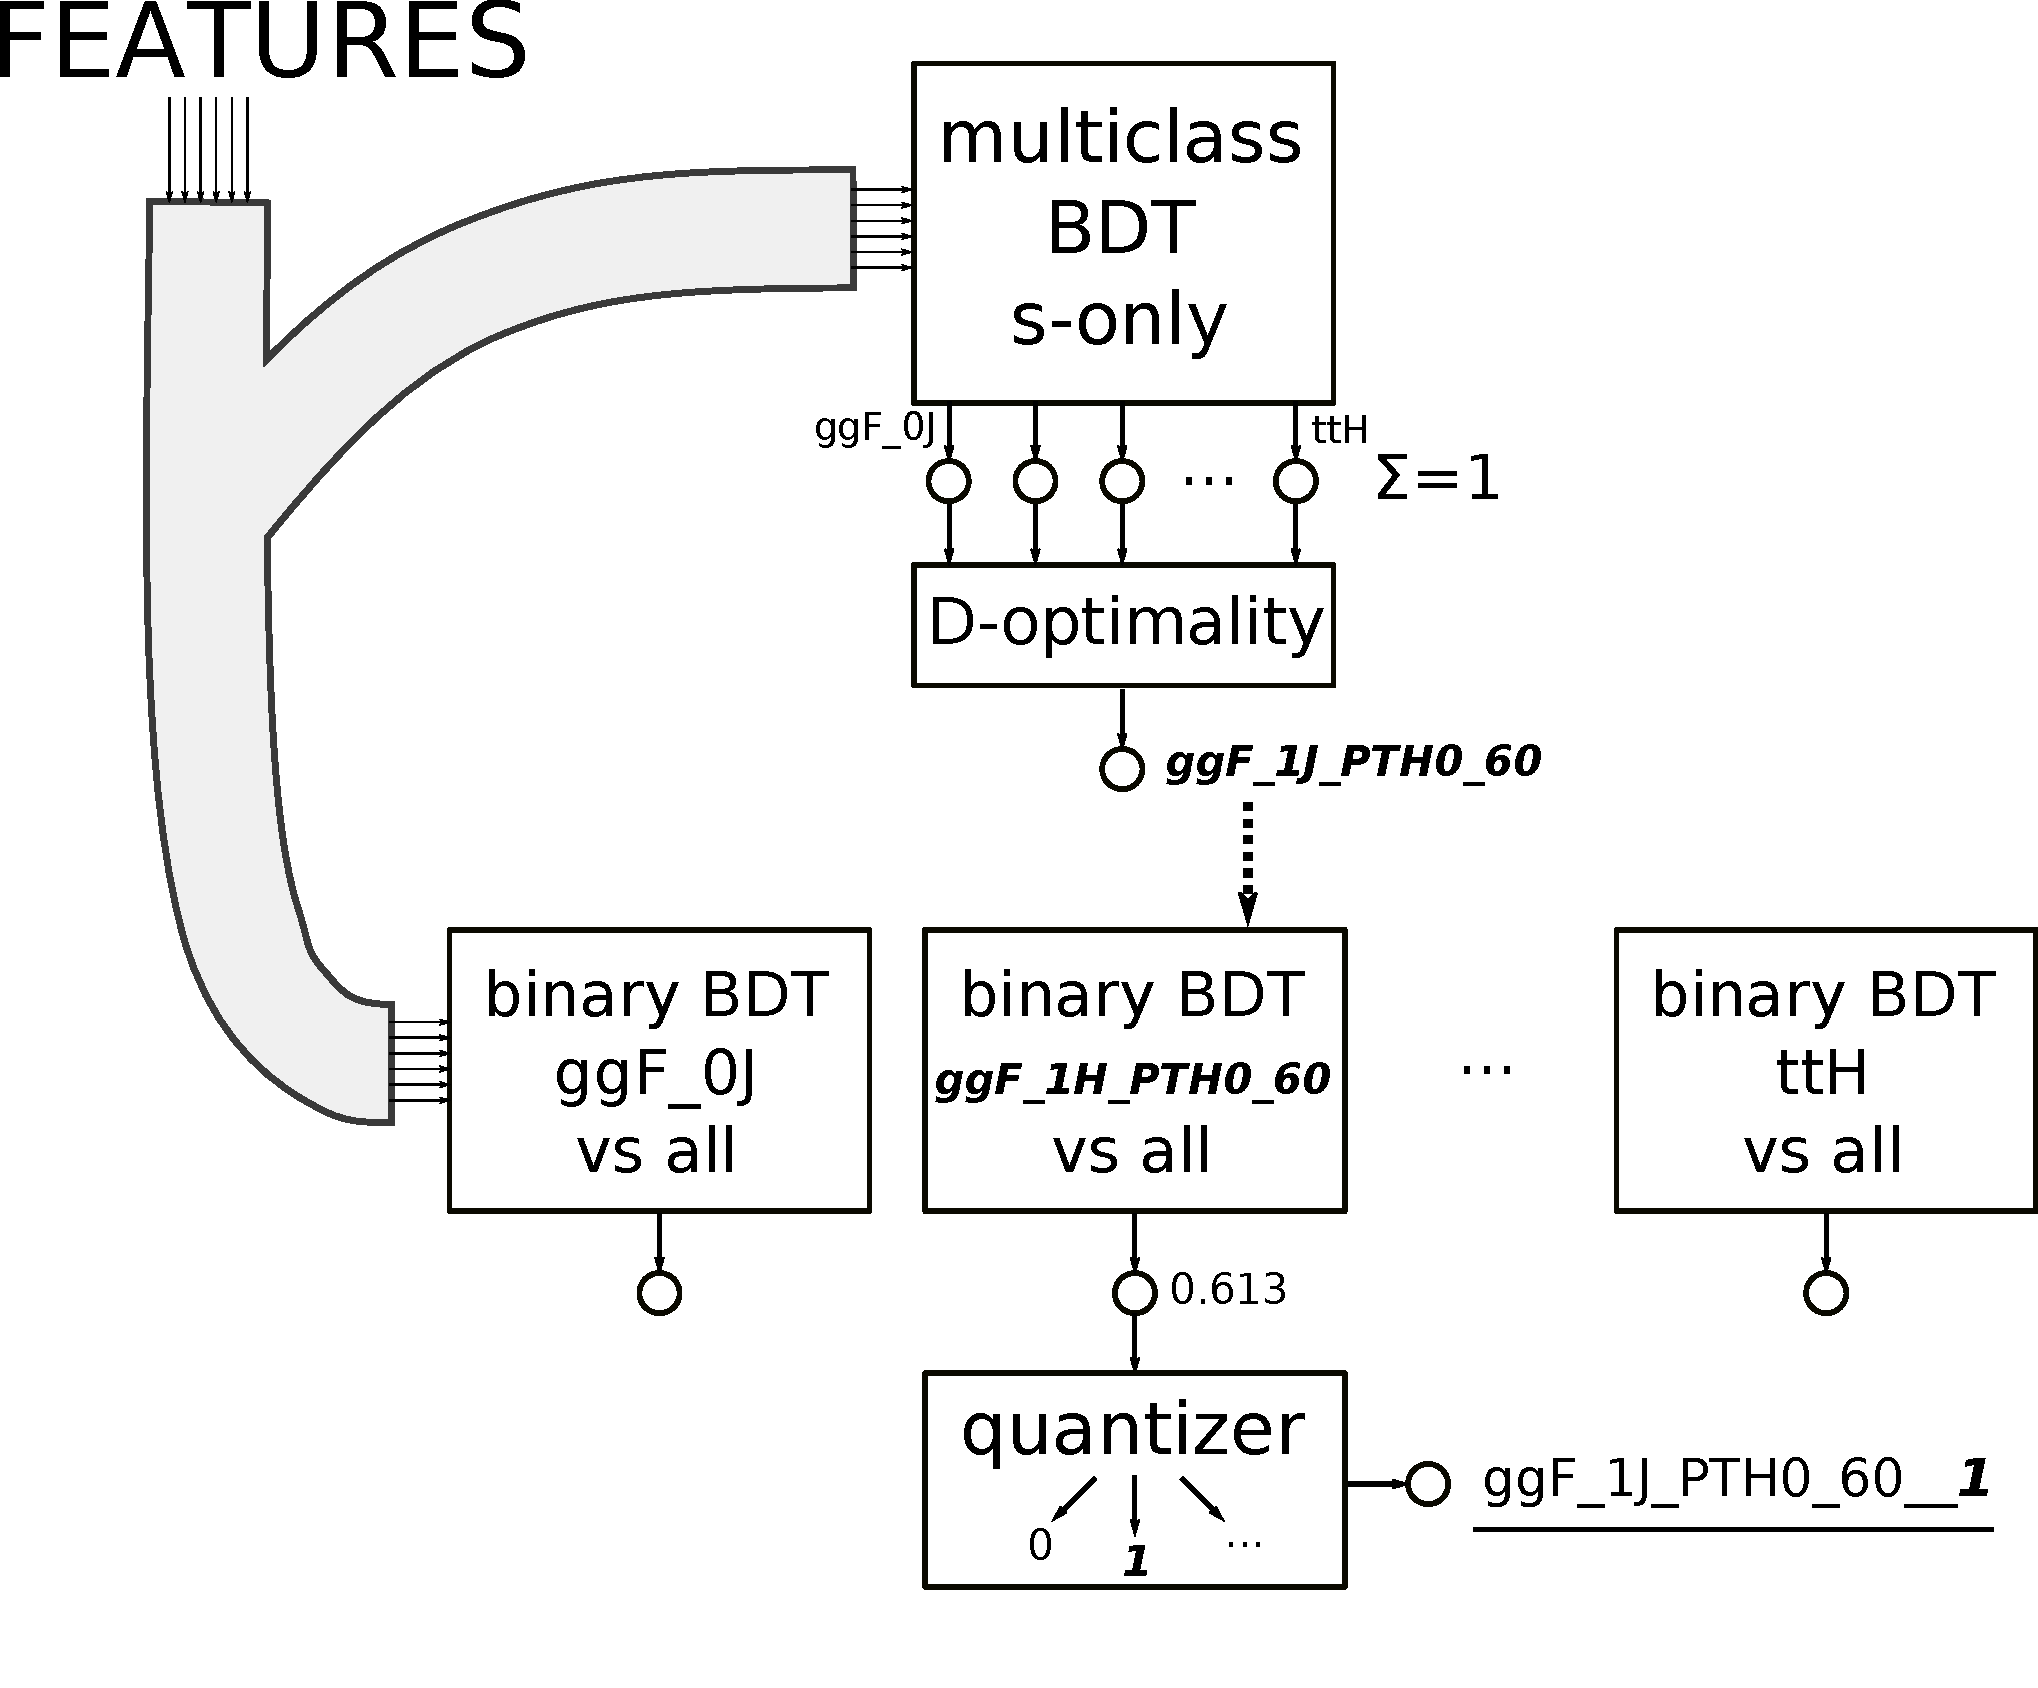
\includegraphics[width=0.7\linewidth]{figures/couplings_chapter/sketch_Dopt.pdf}
  \label{fig:global_cat_sketch}
  \caption{Overview of the categorization approach. The STXS names reported in the cartoon are related to the old STXS 1.0 scheme, but are closely related to the current STXS 1.2 categories.}
\end{figure}

The inputs to all BDTs are kinematic variables for the various objects in an event. In order to avoid sculpting of the shapes used in the statistical analysis, any variable found to be linearly correlated with $m_{\gamma \gamma}$ in the signal or background training samples by 5\% or more is removed from the list of inputs. The list of all variables used as input to both the multiclassifier BDT and the binary BDTs is given in Table \ref{tab:design:trainingvariables}.

\begin{landscape}

\begin{table}[]
\begin{center} \footnotesize
\resizebox{1.25\textwidth}{!}{
\begin{tabular}{|c|c|c|c|c|}
\hline
STXS regions & Multi-class BDT & STXS regions  & Binary BDT  \\ \hline
\multirowcell{11}{$gg\rightarrow H$} &  \multirowcell {45}{di-photon $p_\mathrm{T}$ and absolute rapidity; \\\\ di-jet $p_\mathrm{T}$, mass, $\Delta y$, $\Delta\phi$, $\Delta\eta$ between the 2 jets; \\\\  $p_\mathrm{T}$, mass of $\gamma\gamma+j$ and $\gamma\gamma+jj$, \\\\ $\Delta y$, $\Delta\phi$ between $\gamma\gamma$ and $jj$, \\\\ minimum $\Delta R$ between jets and photons,\\\\ mass of the sum of all jets; \\\\ di-lepton $p_\mathrm{T}$, di-e or di-$\mu$ mass, \\\\ $E^{miss}_\mathrm{T}$, $p_\mathrm{T}$ of lepton + $E^{miss}_\mathrm{T}$; \\\\ $p_T$, $\eta$, $\phi$, mass of top candidates; \\\\ Number of jets, barrel jets ($|\eta|<2.5$), b-jets and leptons; \\\\ leading jet $p_T$, sum $p_\mathrm{T}$ of all jets \\\\ $\sum E^\mathrm{T}$, $E^{miss}_\mathrm{T}$ significance; \\\\ Average interaction per crossing, number of primary vertices} & \multirowcell {22}{individual \\ STXS regions from \\ $gg\rightarrow H$ or \\ $qq'\rightarrow Hqq'$} &  \multirowcell {22}{Multi-class BDT variables, and \\\\ $\Delta\phi$, $\Delta \eta$ between the 2 photons ($\Delta\phi_{\gamma\gamma}$, $\Delta\eta_{\gamma\gamma}$); \\\\ Number of electrons and muons; \\\\  $E^{miss}_\mathrm{T}$, $\sum E^\mathrm{T}$, $E^{miss}_\mathrm{T}$ significance, and \\\\ ${E^{miss}_\mathrm{T}}$ azimuthal angle computed from hardest vertex;
\\\\ ($p_\mathrm{Tt}^{\gamma\gamma}$), the component of $\gamma\gamma \vec{p}_\mathrm{T}$ orthogonal to the diphoton thrust axis (unit $\vec{n}$ for which \max_{\hat{n}}\frac{\sum_{i}|\hat{p^{\gamma}_{i}}\dot\hat{n}|}{\sum_{i}|\hat{p^{\gamma}_{i}}|});
\\\\ Half of the difference between di-photon $\eta$ and sum $\eta$ of leading 2 jets ($\eta^{Zepp}$);
\\\\ $\phi^{*}_{\gamma\gamma} = \tan(\frac{\pi-|\Delta\phi_{\gamma\gamma}|}{2}) \sqrt{1-\tanh^{2}(\frac{\Delta\eta_{\gamma\gamma}}{2})}$
\\\\ $\cos\theta^{*}_{\gamma\gamma}= |\frac{(E^{\gamma_1} + p_z^{\gamma_1}) \cdot (E^{\gamma_2} - p_z^{\gamma_2}) -  (E^{\gamma_1} - p_z^{\gamma_1}) \cdot (E^{\gamma_2} + p_z^{\gamma_2})} { m_{\gamma\gamma} + \sqrt{(m_{\gamma\gamma}^2 + (p_\mathrm{T}^{\gamma\gamma})^2)} }|$} \\
 & & & \\
  & & &\\
    & & &\\
     & & & \\
     & & & \\
     & & & \\
      & & & \\
       & & & \\
        & & & \\
         & & & \\
\cline{1-1}
\multirowcell{11}{$qq'\rightarrow Hqq'$} & &  &    \\
 & & & \\
    & & &\\
     & & & \\
     & & & \\
      & & & \\
       & & & \\
       & & &\\
       & & & \\
        & & & \\
         & & & \\
\cline{1-1} \cline{3-4}
\multirowcell{7}{$qq\rightarrow H\ell\nu$} &  & \multirowcell{7}{\WH \\ STXS regions\\ combined} &  \multirowcell {14}{$p_\mathrm{T}/m_{\gamma\gamma}$, $\eta$, $\phi$ of 2 leading photons; \\\\ $p_\mathrm{T}$, $\eta$, $\phi$ of 2 leading leptons; \\\\ $E^{miss}_\mathrm{T}$, $E^{miss}_\mathrm{T}$ significance, ${E^{miss}_\mathrm{T}}$ azimuthal angle;
\\\\ Whether or not the ${E^{miss}_\mathrm{T}}$ built from di-photon vertex is \\\\ larger than that built from the hardest vertex \\ by more than 30 GeV;
\\\\ di-lepton mass, and transverse mass of lepton + ${E^{miss}_\mathrm{T}}$}   \\
& & &\\
  & & &\\
    & & &\\
        & & &\\
            & & &\\
              & & &\\
\cline{1-1} \cline{3-3}
\multirowcell{7}{$qq\rightarrow H\ell\ell$} &  & \multirowcell{7}{\ZH \\ STXS regions \\ combined} &    \\
& & &\\
  & & &\\
    & & &\\
        & & &\\
            & & &\\
              & & &\\
\cline{1-1} \cline{3-4}
\multirowcell{8}{$t\bar{t}H$} & & \multirowcell{8}{$t\bar{t}H$ \\ STXS regions \\ combined} & \multirowcell {9}{$p_\mathrm{T}$, $\eta$, $\phi$ of 2 leading photons; \\\\ $p_\mathrm{T}$, $\eta$, $\phi$ and B-tagging scores of 6 leading jets;\\\\ $E^{miss}_\mathrm{T}$, $E^{miss}_\mathrm{T}$ significance, ${E^{miss}_\mathrm{T}}$ azimuthal angle; \\\\ Top reconstruction BDT scores}   \\
    & & &\\
        & & &\\
            & & &\\
              & & &\\
        & & &\\
            & & &\\
                & & &\\
            \cline{1-1}  \cline{3-3}
   $tH$   & & $tWH$, $tHjb$ &\\
\hline
\end{tabular}
}
\caption{List of training variables used for the multiclass and binary BDTs.}

\label{tab:design:trainingvariables}

\end{center}
\end{table}
\end{landscape}

To train the multiclassifier BDT, all signal samples are merged ($ggF$, $VH$, $VBF$, $ttH$, $tH$). A weight is then applied to each event such that all processes have equal yields in the training sample (that is, so processes such as $tH$ with a small cross-section are not underrepresented). The output of the multiclassifier BDT is a 44-dimensional vector discriminant with an index $y_{i}$ for each truth bin; these indices are then converted into class probabilities $z_{i}$ using a softmax function: $z_{i} = e^{y_{i}}/{\Sigma_{j}e^{y_{j}}}$. The BDT is trained by minimizing the cross-entropy of the softmax $z_{i}$ using the LightGBM package \ref{cite:LightGBM}.

After this, a per-class weight is calculated for each category using a so-called 'D-optimality' procedure. This is done iteratively: first, weights are initialized to $w_{i} = 1$. Second, events are classified based on the value of $w_{i}z_{i}$. An Asimov dataset \ref{cite:Asimov} is then created using the signal samples in each category, normalized to their Standard Model cross-sections and simulated continuum background ($\gamma\gamma$, $V\gamma\gamma$, and $tt\gamma\gamma$) scaled to the TI sidebands in the region $95 GeV < m_{\gamma \gamma} < 105 GeV$. A simplified version of the overall fit is then performed, using an exponential function if the total scaled background yield is determined to be less than 400 events and an ExpPoly2 function otherwise. This Asimov dataset is then fitted, leading to a covariance matrix C of the event yields in each region. The weights are then iteratively updated using the Powell algorithm \ref{cite:Powell1}, \ref{cite:Powell2} until the determinant of the covariance matrix is minimized. By minimizing the determinant of this covariance matrix, the information gain from a particular classification scheme is maximized \ref{cite:Linley}. In an experimental sense, this corresponds to higher signal purity in the classes corresponding to rare processes such as $ttH$ and $tH$. These final weights are multiplied by the softmax function output; events are classified based on their maximum value of $w_{i}z_{i}$. This produces 44 classes, one for each STXS region. The multiclassifier output for four representative classes is shown in Figure \ref{fig:design:BDT_outputs_multiclass}.


\begin{figure}[!htbp]
\centering
\subfloat[\ggtoH\ (1-jet, $120 \le~\ptH \le 200\,\GeV$)]{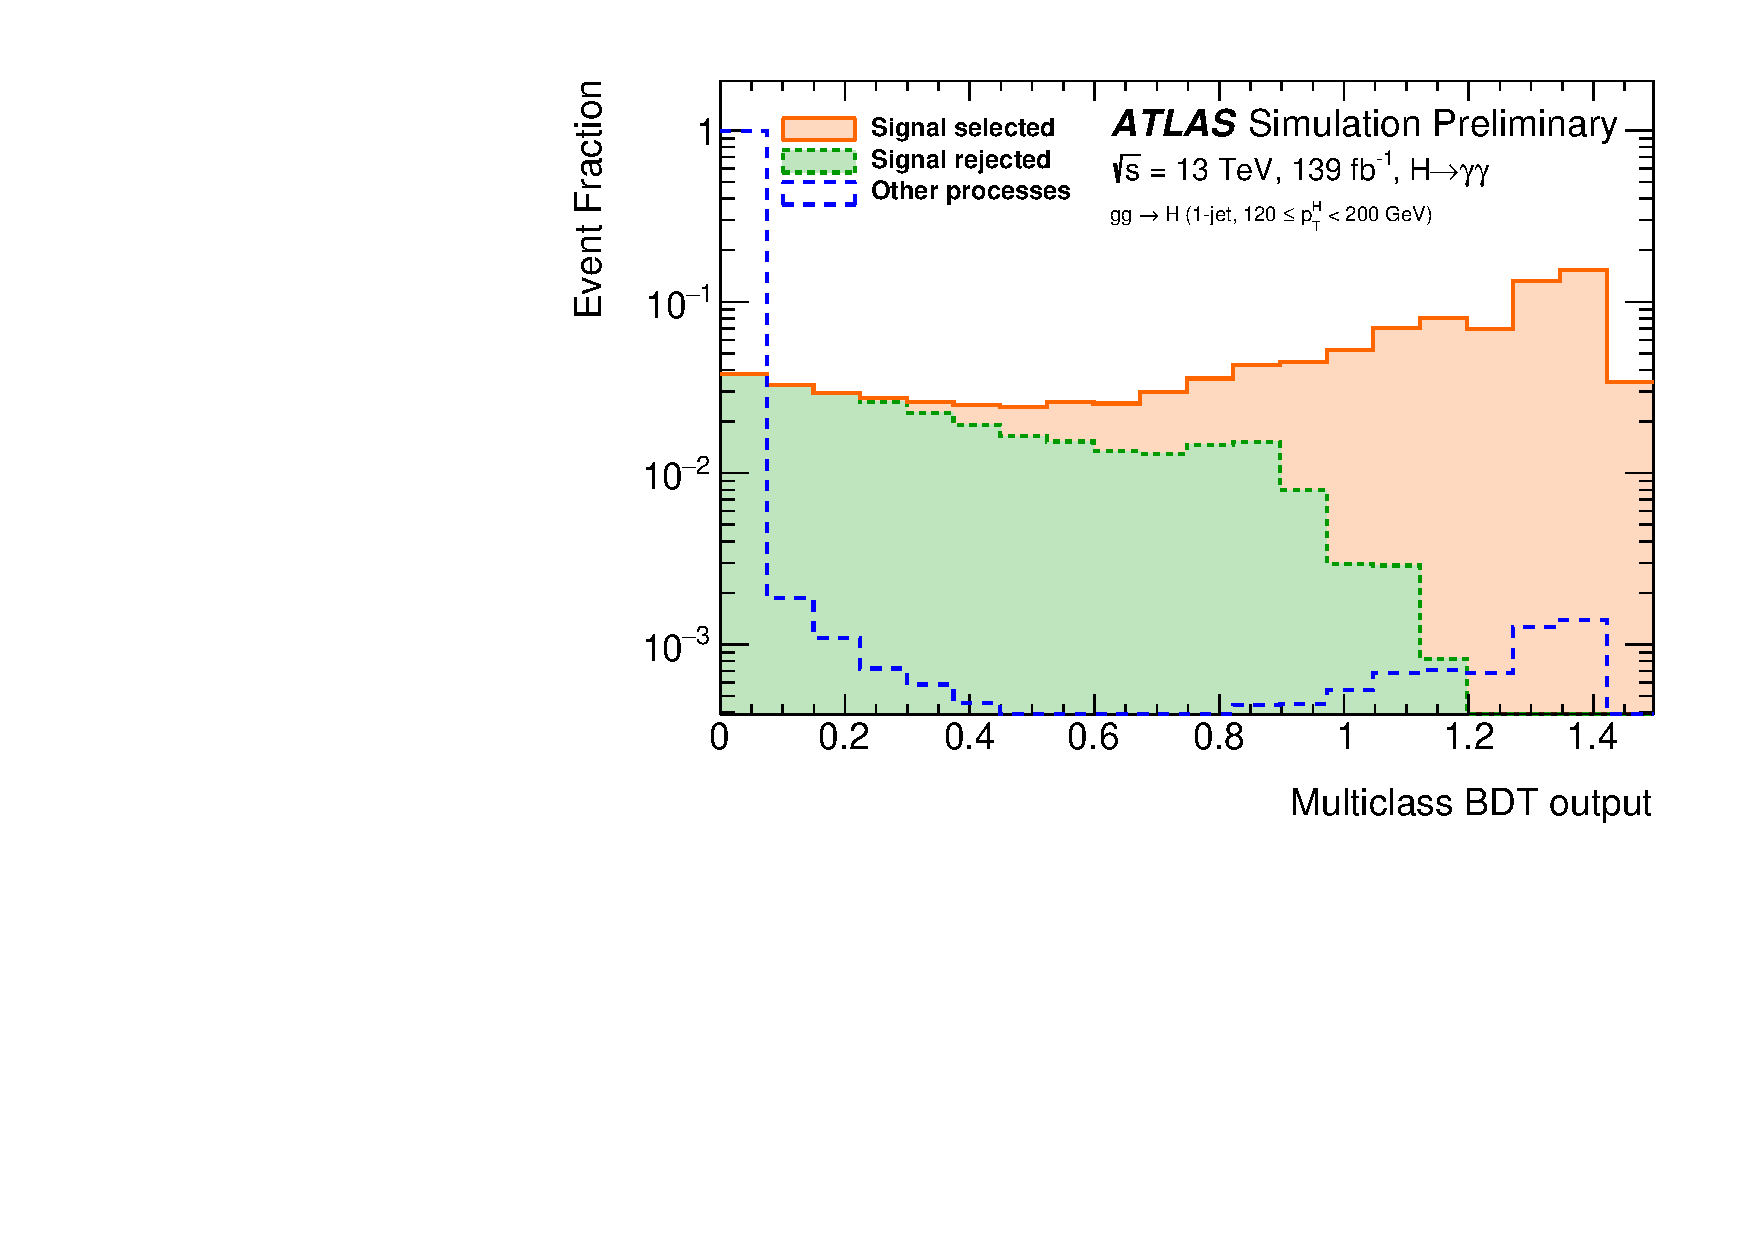
\includegraphics[width=0.49\linewidth]{figures/couplings_chapter/multiclass_GG2H_1J_PTH_120_200.pdf}\label{fig:design:BDT_ggH:multiclass}}
\subfloat[\qqtoHqq\ ($\ge 2$-jets, $\mjj > 700\,\GeV$, $\ptHjj > 25\,\GeV$)]{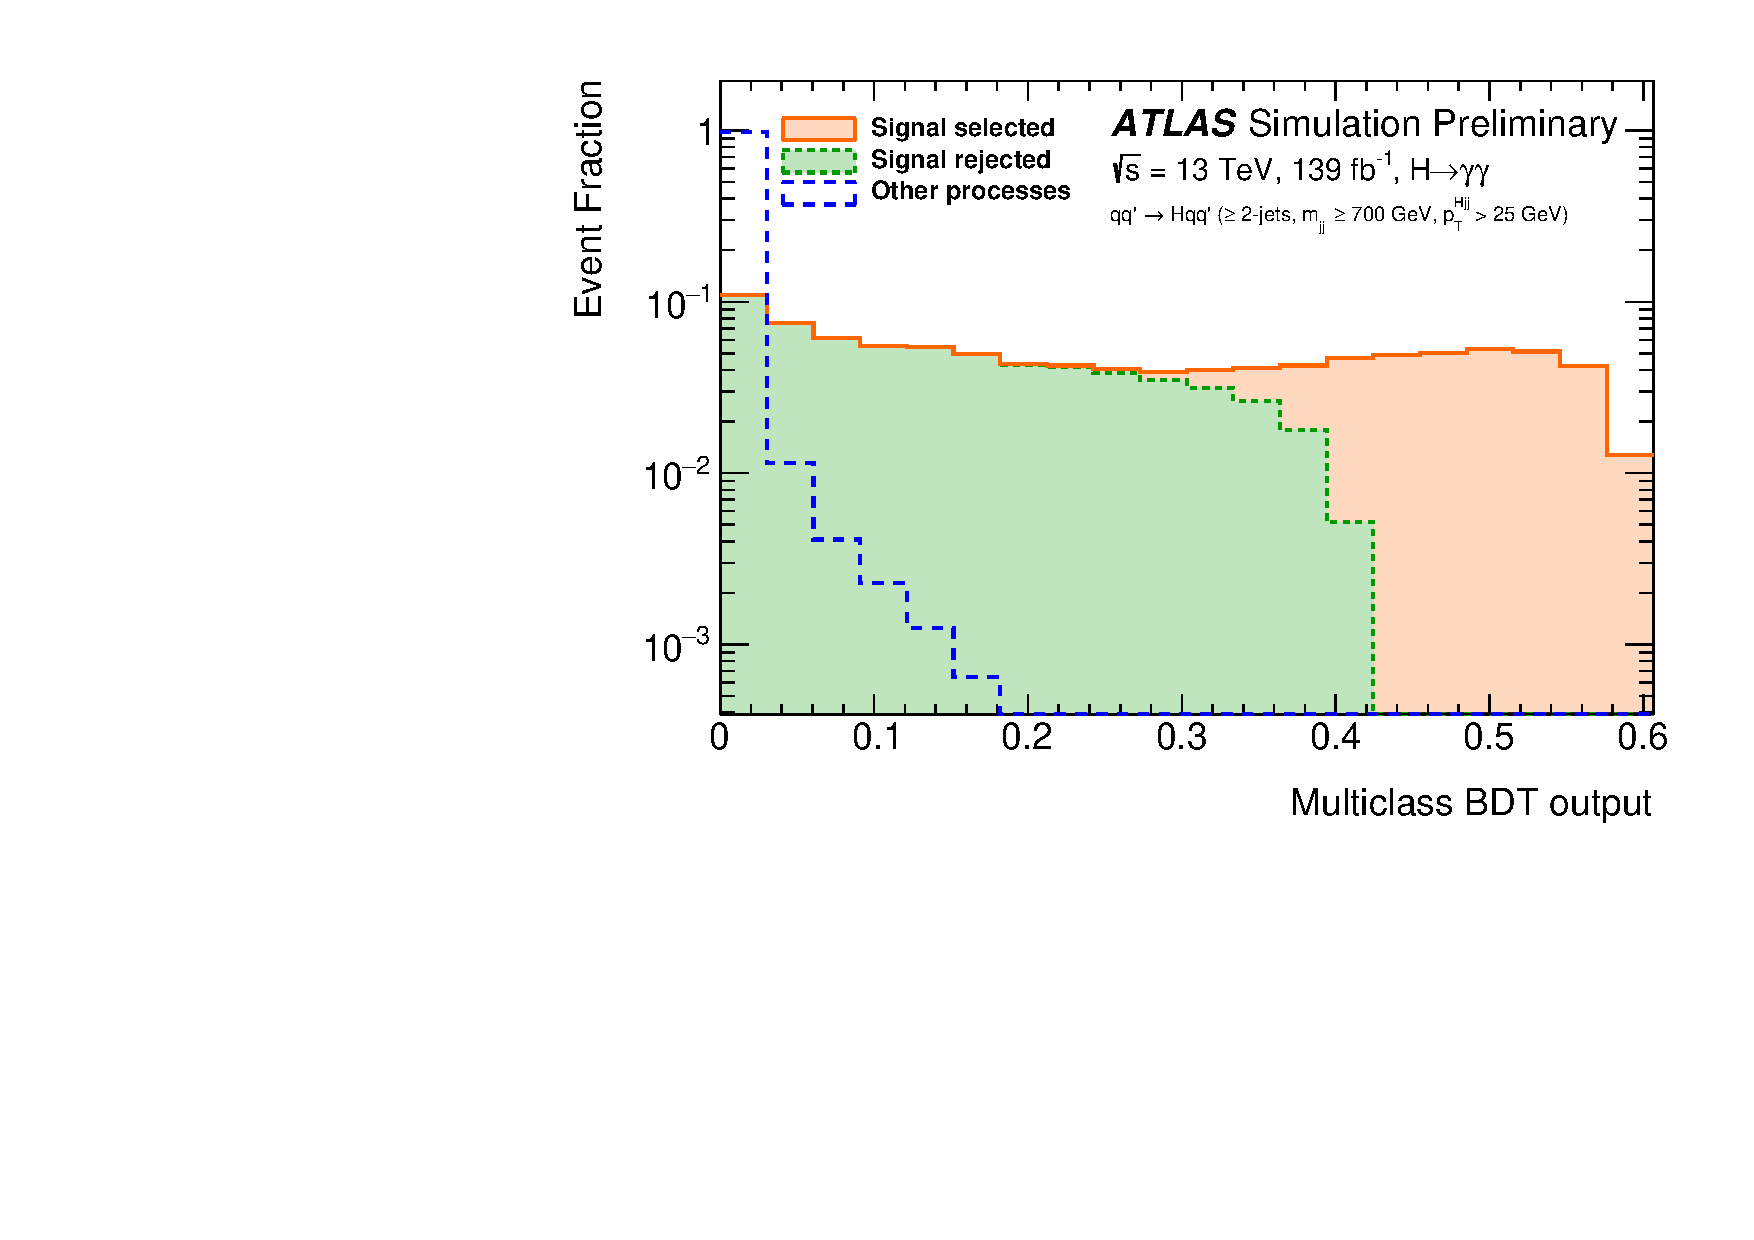
\includegraphics[width=0.49\linewidth]{figures/couplings_chapter/multiclass_QQ2HQQ_GE2J_MJJ_GT700_PTH_0_200_PTHJJ_0_25}\label{fig:design:BDT_VBF:multiclass}}\\
\subfloat[\qqtoHln\ ($75 \le \ptH < 150\,\GeV$)]{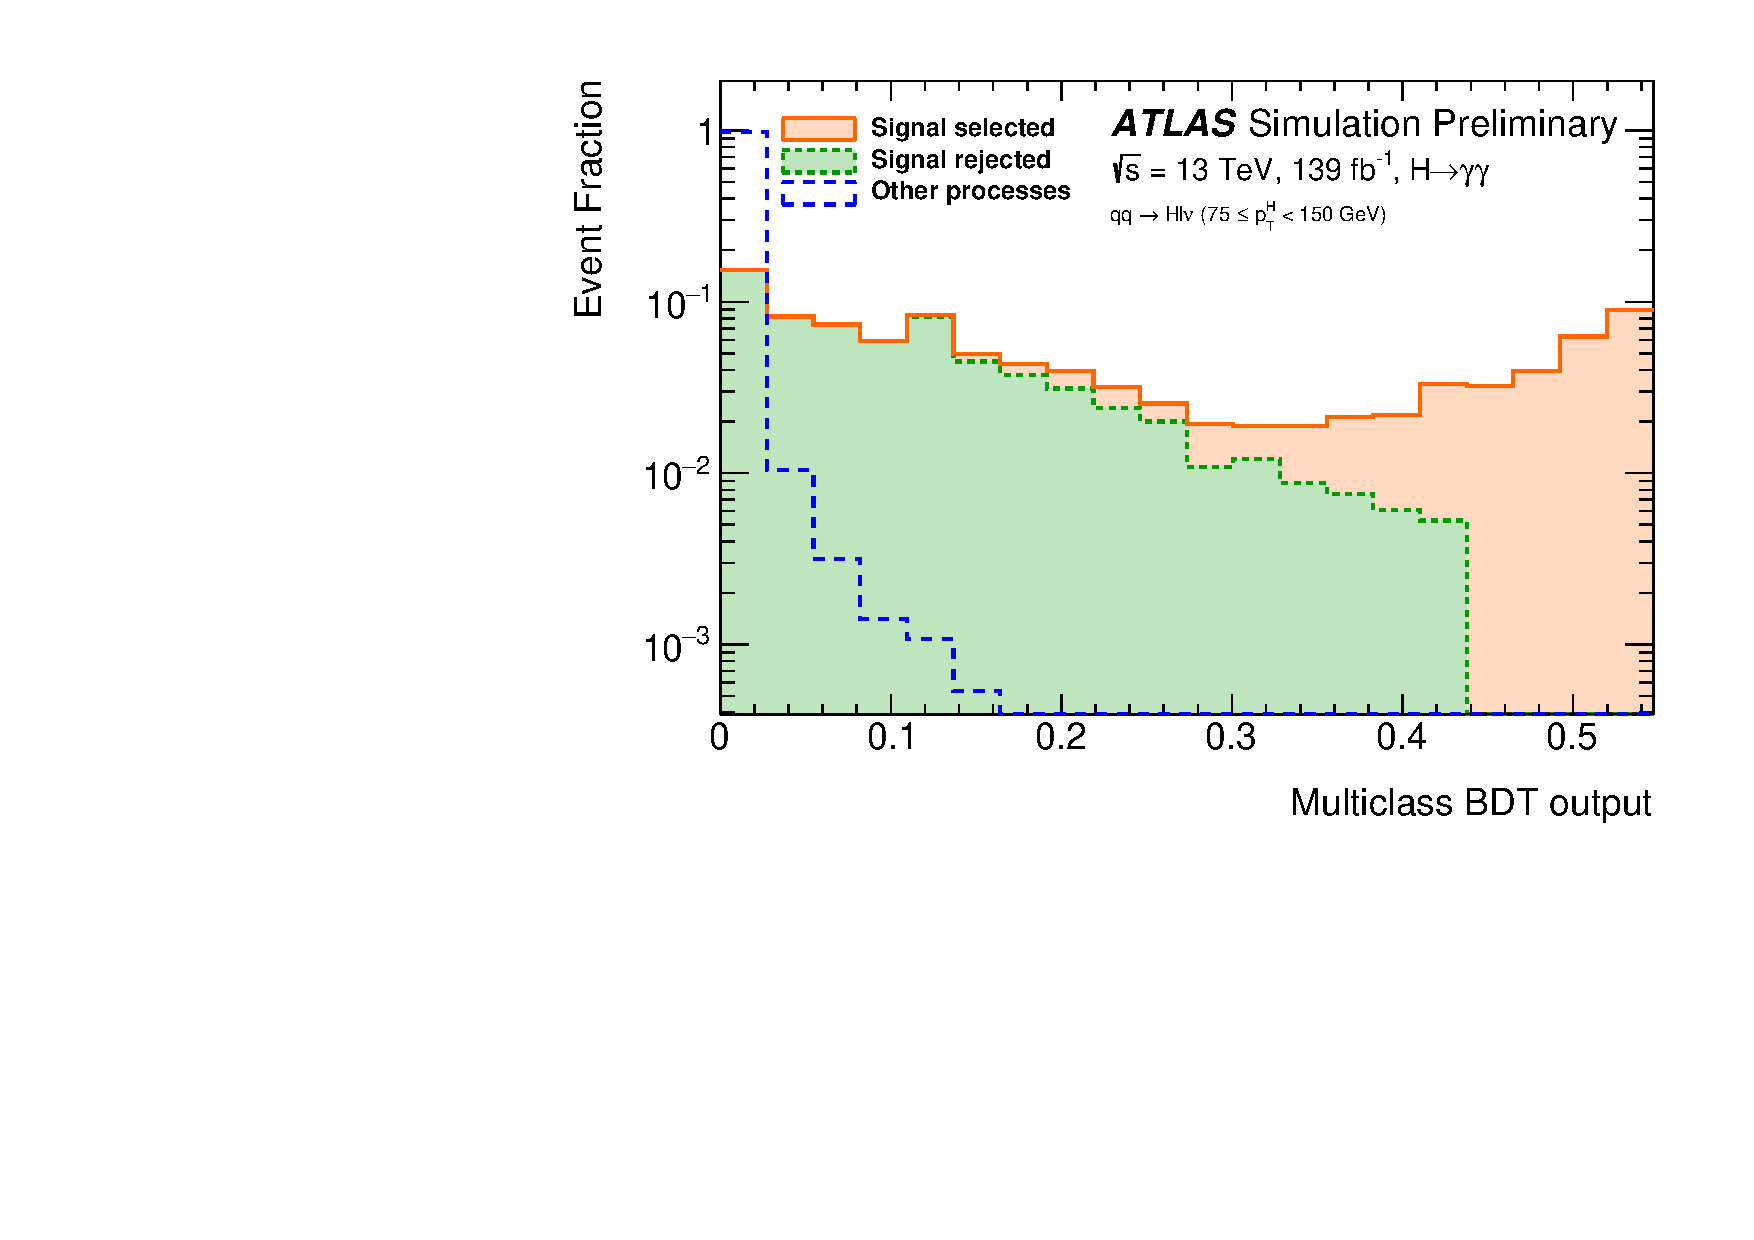
\includegraphics[width=0.49\linewidth]{figures/couplings_chapter/multiclass_QQ2HLNU_PTV_75_150} \label{fig:design:BDT_VH:multiclass}}
\subfloat[\ttH\ ($60 \le \ptH < 120\,\GeV$)  ]{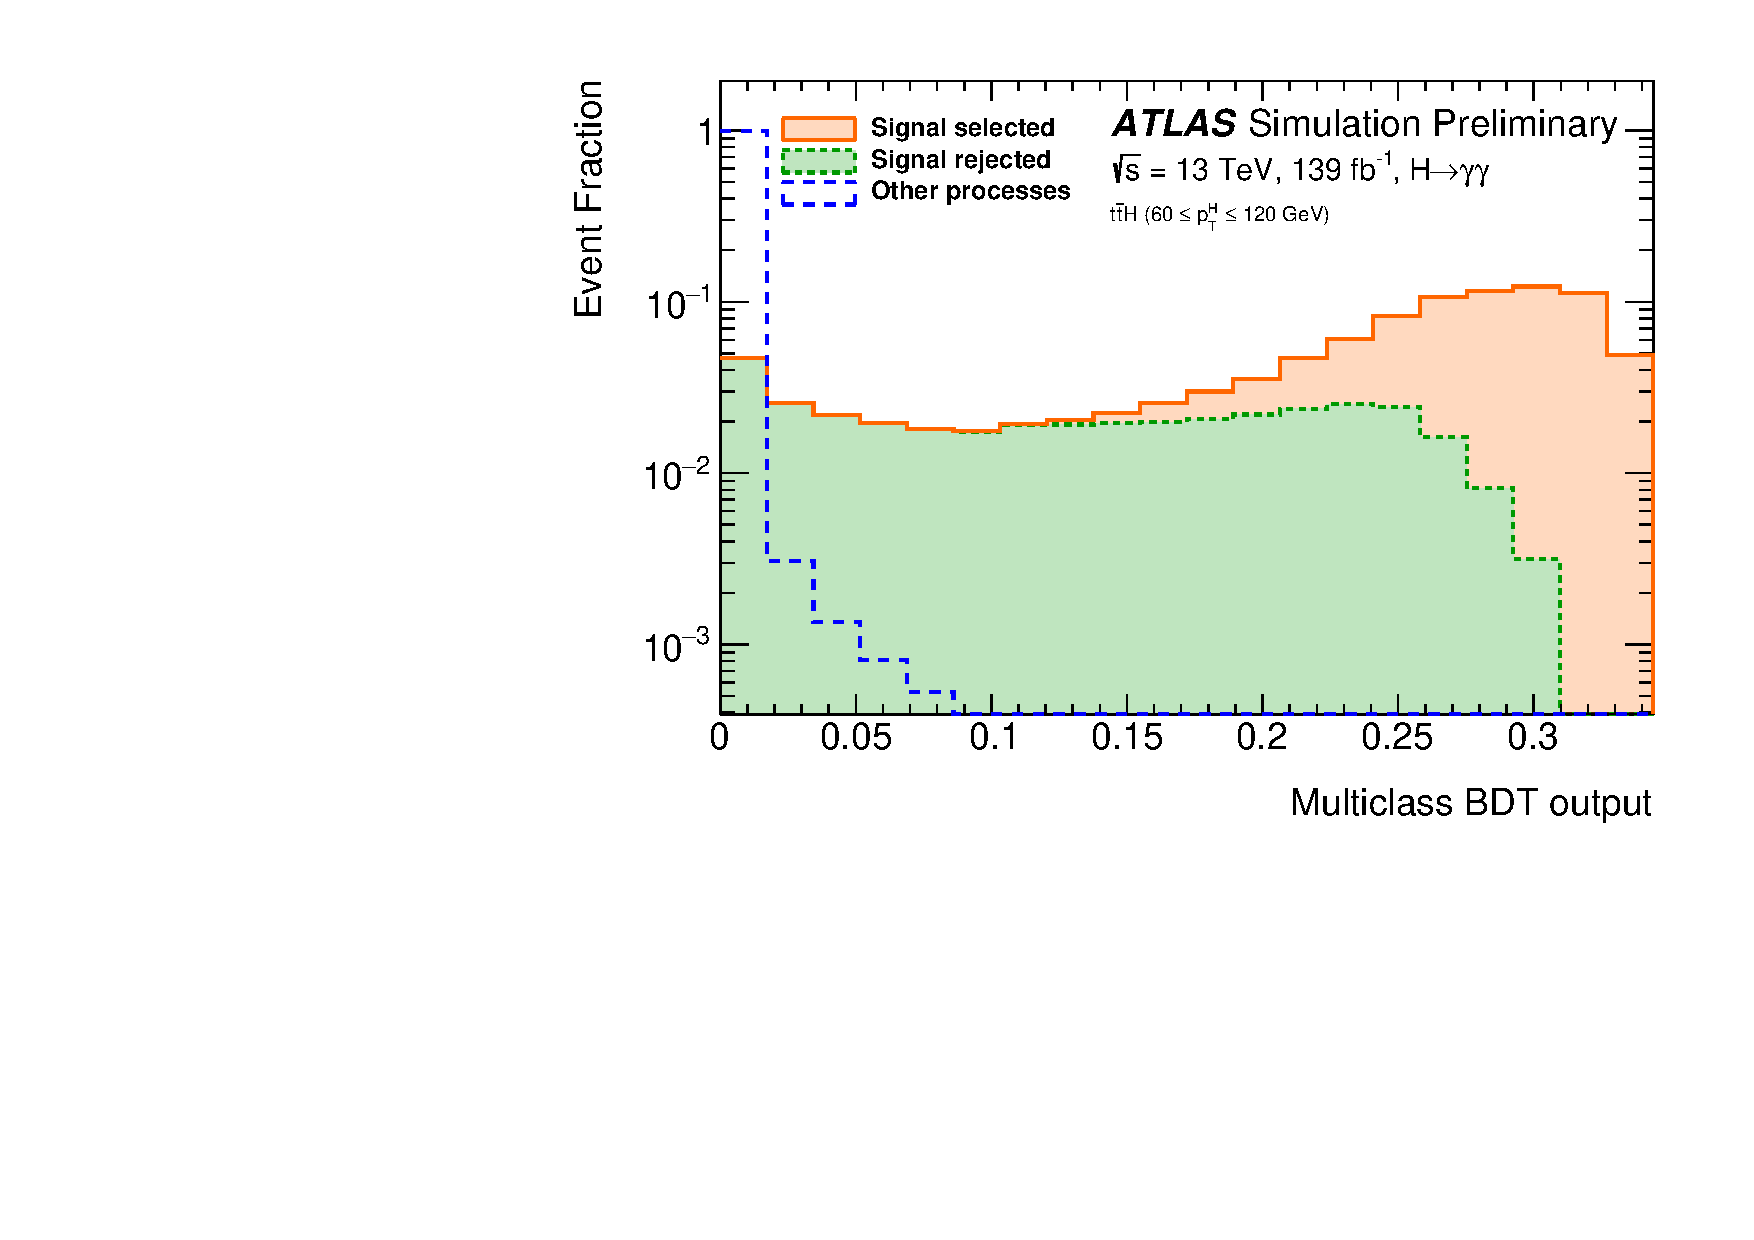
\includegraphics[width=0.49\linewidth]{figures/couplings_chapter/multiclass_TTH_PTH_60_120}\label{fig:design:BDT_ttH:multiclass}}
\caption{Multiclassifier output distributions for four STXS classes. In each plot, the multiclassifier output distribution is shown for events corresponding to the target STXS truth bin (solid) and events in other STXS truth bins (dashed). The target STXS bin is further broken down into the subset of events passing the multiclassifier selection (orange), and the subset of events that fail it (green).}
\label{fig:design:BDT_outputs_multiclass}
\end{figure}

After being sorted into a multiclass region, events are then passed through a binary signal-or-background BDT that is trained independently for each category. For classes targeting $ggH$ and $qq' \rightarrow Hqq'$ (that is, $VBF$ and hadronic $VH$), a binary BDT is trained for each class, using the targeted process as signal and the other Higgs processes and continuum diphoton production as background. However, a single binary BDT is trained for all leptonic $VH$ classes and another is trained for all $ttH+tH$ classes due to a lack of training statistics if no merging is applied. For the leptonic $VH$ and the $ttH+tH$ binary BDTs, NTI data is used to model the background.

In each class, events are then sorted into a final set of 88 total categories based on the binary BDT scores. Each of the initial 44 classes is subdivided into one, two, or three categories, depending on the targeted process. The category boundaries are found by scanning all possible sets of boundaries in binary BDT score and choosing the set that maximizes the Poisson Number-Counting Significance, defined as $\sqrt{2((S+B)\ln(1+S/B)-S)}$ as in section \ref{sec:ttHCP_chapter}. The signal S for this significance metric is the yield of the targeted STXS bin, while the background is comprised of both a continuum diphoton contribution calculated from Sherpa Monte Carlo events scaled to the TI sidebands in the region $95 GeV < m_{\gamma \gamma} < 105 GeV$ and Higgs events from other STXS bins. A class is split into two categories if it able to achieve a significance gain of more than 5\% over the single-category case, and a further third category if it able to achieve an additional 5\% significance gain over the two-category case by doing so. Some events may have binary BDT scores causing them to fall outside the subdivided regions; for these events, three 'unselected' categories (one for $qq \rightarrow H l \nu$, one for $qq \rightarrow ZH$, and one for $ttH+tH$) are created. The binary BDT distribution in the same four representative classes as previously described is shown in Figure \ref{fig:design:BDT_outputs_binary}.


\begin{figure}[!htbp]
\centering
\subfloat[\ggtoH\ (1-jet, $120 \le~\ptH < 200\,\GeV$)]{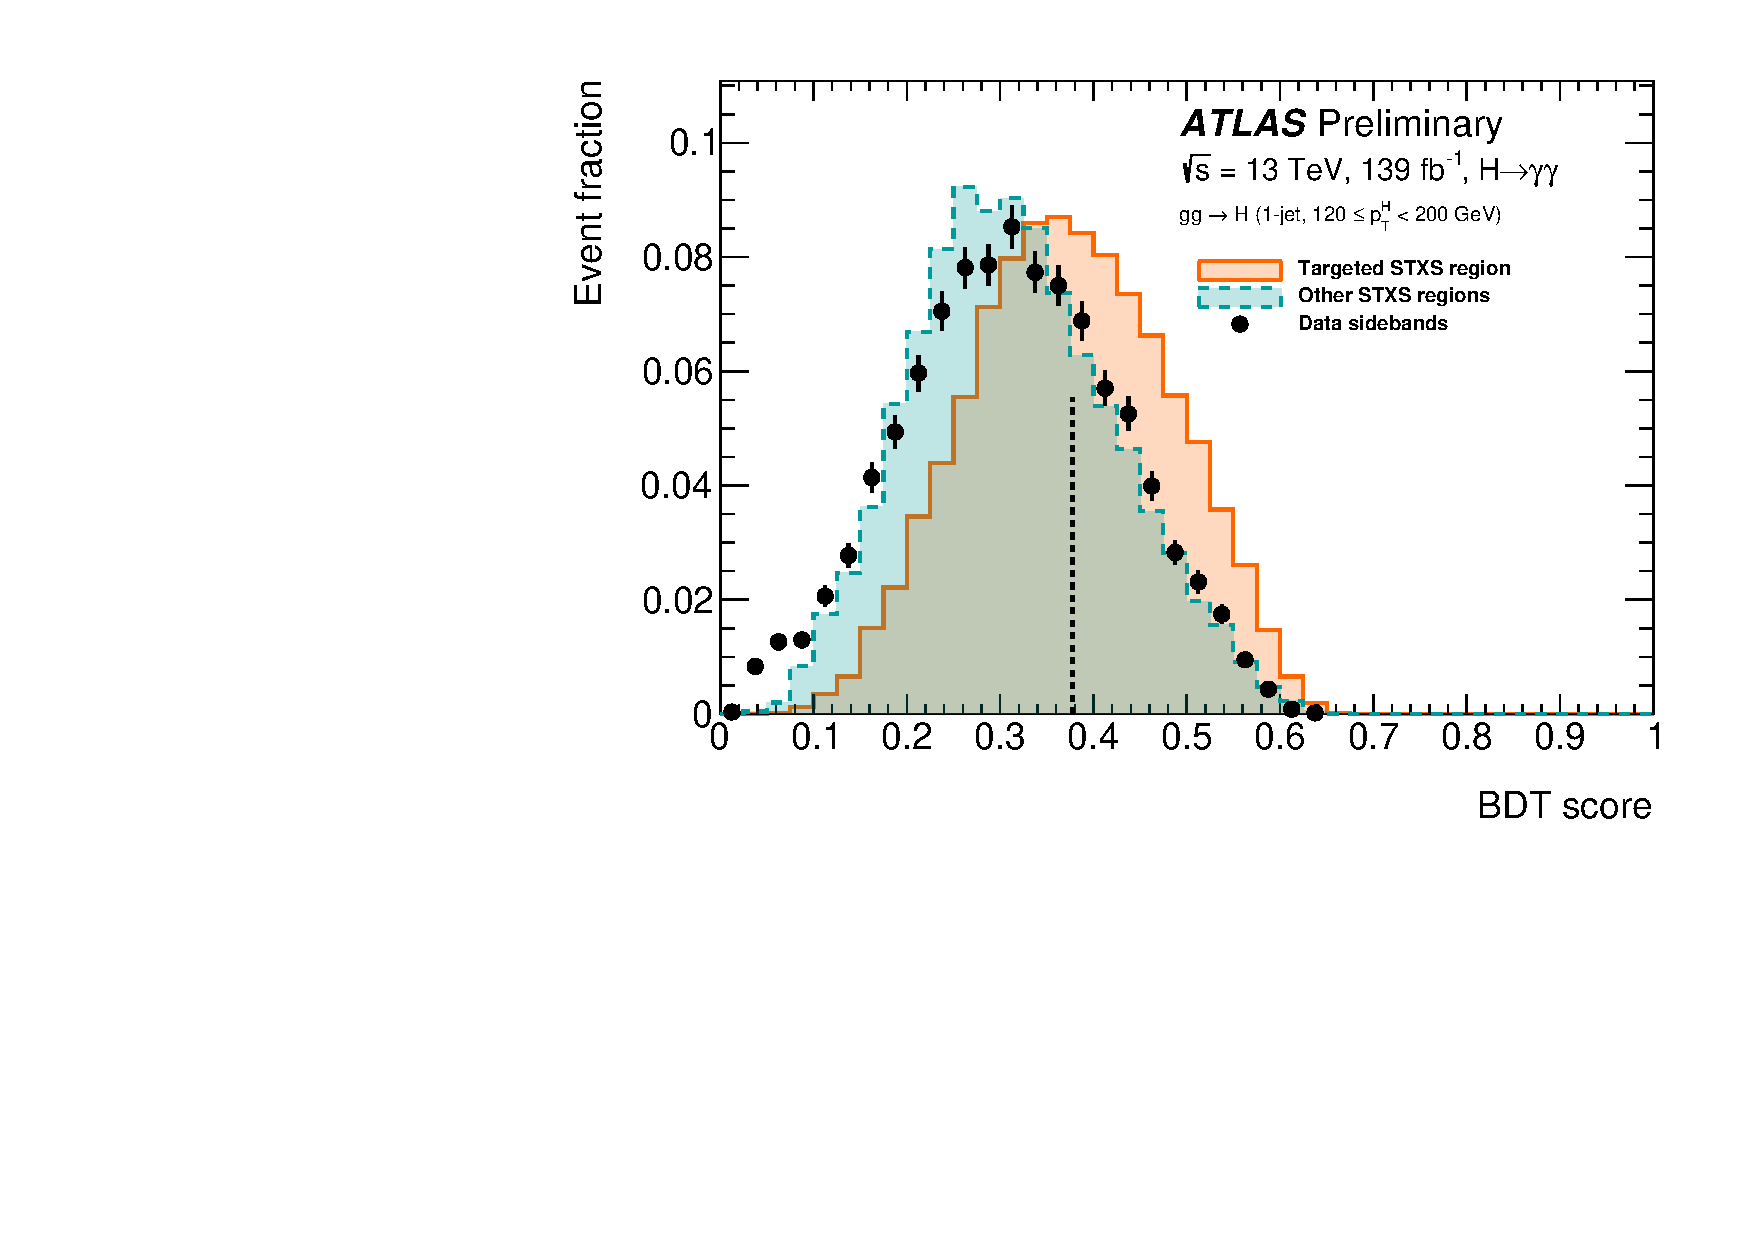
\includegraphics[width=0.49\linewidth]{figures/couplings_chapter/BDT2score_GG2H_1J_PTH_120_200.pdf}\label{fig:design:BDT_ggH:binary}}
\subfloat[\qqtoHqq\ ($\ge 2$-jets, $\mjj > 700\,\GeV$, $\ptHjj > 25\,\GeV$)]{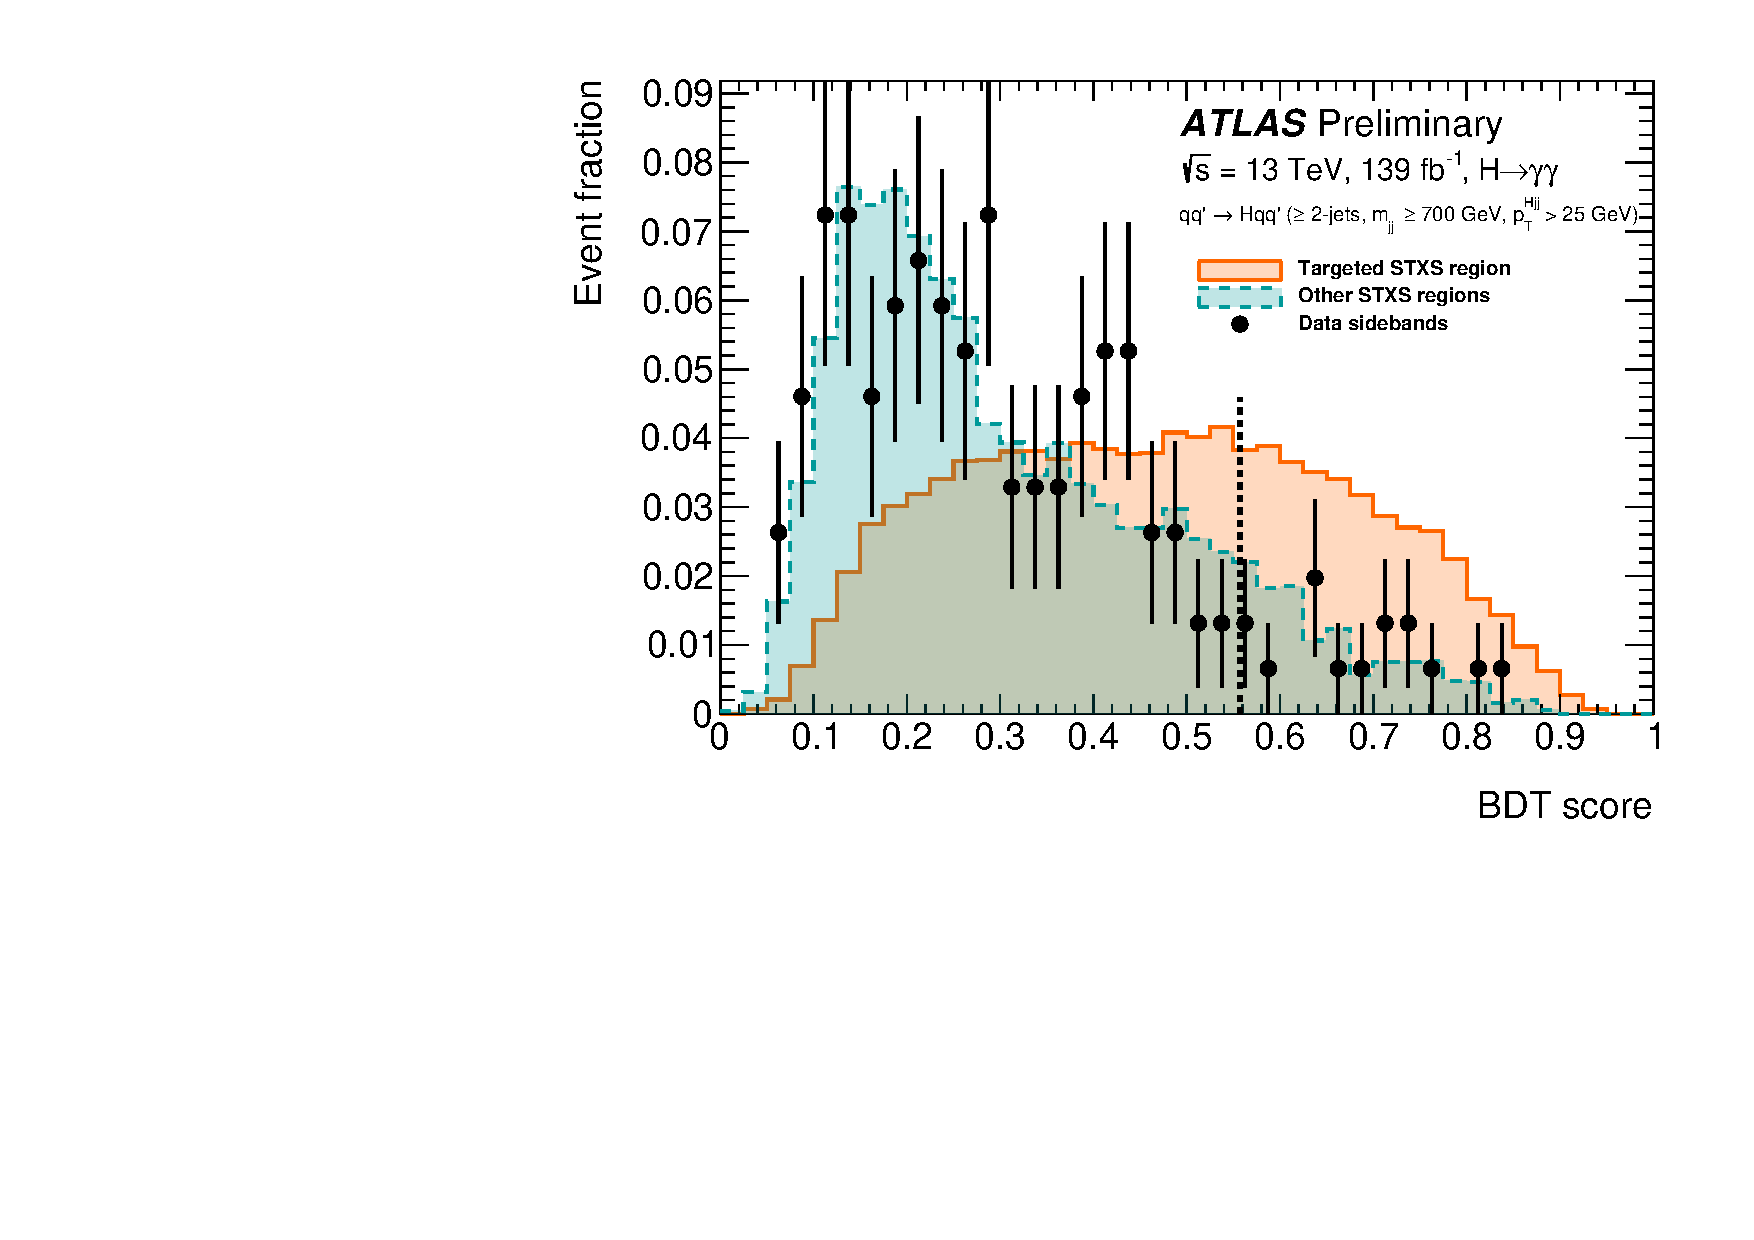
\includegraphics[width=0.49\linewidth]{figures/couplings_chapter/BDT2score_QQ2HQQ_GE2J_MJJ_GT700_PTH_0_200_PTHJJ_0_25}\label{fig:design:BDT_VBF:binary}}	\\
\subfloat[\qqtoHln\ ($75 \le \ptH < 150\,\GeV$)]{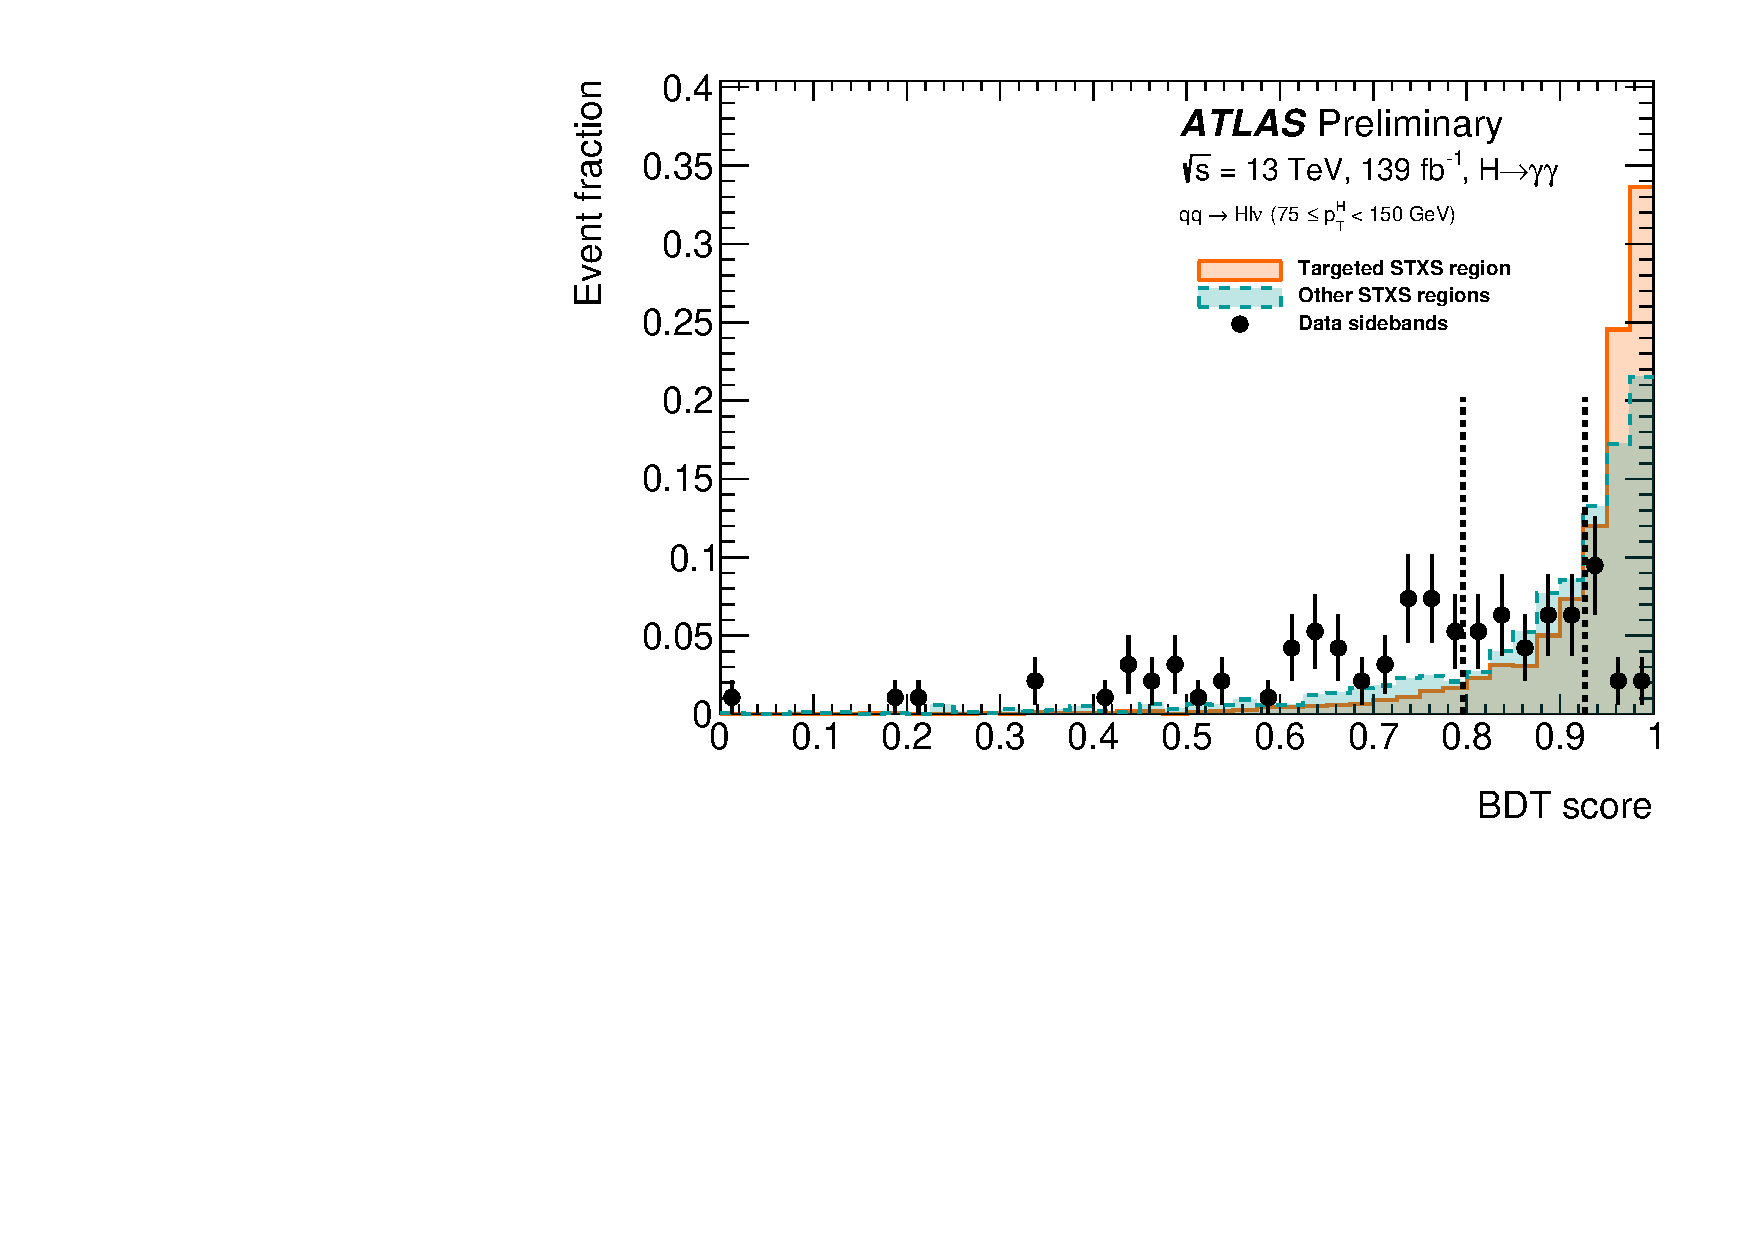
\includegraphics[width=0.49\linewidth]{figures/couplings_chapter/BDT2score_QQ2HLNU_PTV_75_150}\label{fig:design:BDT_VH:binary}}
\subfloat[\ttH\ ($60 \le \ptH < 120\,\GeV$)]{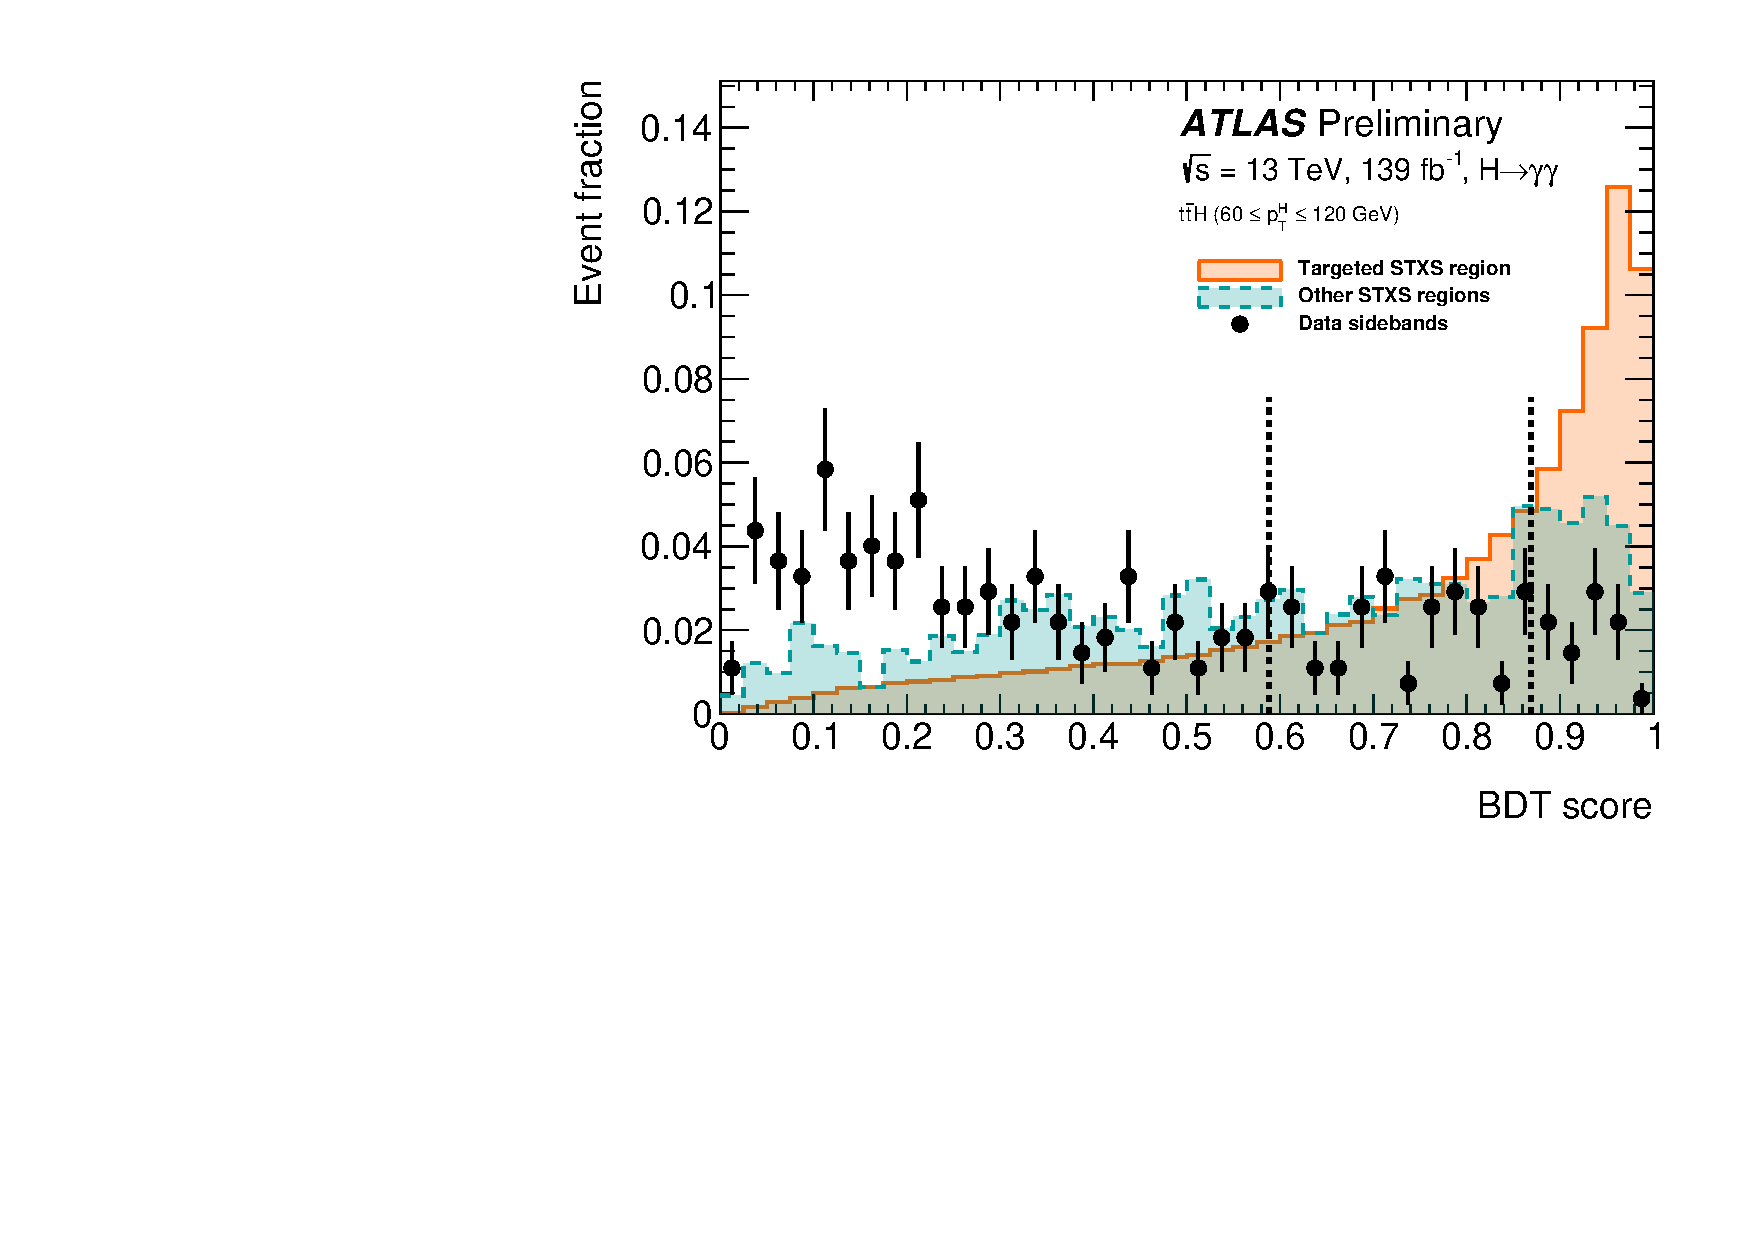
\includegraphics[width=0.49\linewidth]{figures/couplings_chapter/BDT2score_TTH_PTH_60_120}\label{fig:design:BDT_ttH:binary}}
\caption{Binary BDT distributions in four STXS classes. For each class, the binary BDT output distribution is shown for the target STXS truth bin (solid), other STXS truth bins (dashed), and background (dots) represented by the events in the diphoton mass sidebands (105 $<~m_{\gamma \gamma}~<~$ 120 GeV or 130 $<~m_{\gamma \gamma}~<~$ 160 GeV). The vertical lines indicate the boundaries of the analysis categories. }
\label{fig:design:BDT_outputs_binary}
\end{figure}


The expected yield, purity ($S/(S+B)$), and significance for each category is given in Table \ref{tab:design:yields}. The correspondence between the reconstructed categories and the STXS truth bins is given in Figure \ref{fig:design:yields}.

\begin{table}[]
    \centering
    \resizebox{0.49\textwidth}{!}{
    \adjustbox{valign=t}{
    \begin{tabular}{l|c|c|c|c}
                                    Category  &      $S$  &  $B$  &  $f$  &  $Z$ \\
\hline
\multicolumn{5}{c}{\ggtoH}\\
\tabggHjPt{0}{}{10}{}               &   730  &    24000  &  0.03  &   4.6 \\
\tabggHjPt{0}{10}{200}{}            &  2200  &    66000  &  0.03  &   8.4 \\
\tabggHjPt{1}{}{60}{}               &   550  &    16000  &  0.03  &   4.4 \\
\tabggHjPt{1}{60}{120}{}            &   470  &    10000  &  0.04  &   4.7 \\
\tabggHjPt{1}{120}{200}{High}       &    37  &      250  &  0.13  &   2.3 \\
\tabggHjPt{1}{120}{200}{Med}        &    50  &      620  &  0.07  &   2.0 \\
\tabggHmPt{}{350}{}{60}{High}       &    39  &     1200  &  0.03  &   1.1 \\
\tabggHmPt{}{350}{}{60}{Med}        &   120  &     5300  &  0.02  &   1.6 \\
\tabggHmPt{}{350}{}{60}{Low}        &   490  &    19000  &  0.03  &   3.6 \\
\tabggHmPt{}{350}{60}{120}{High}    &    36  &      370  &  0.09  &   1.8 \\
\tabggHmPt{}{350}{60}{120}{Med}     &   110  &     2300  &  0.05  &   2.2 \\
\tabggHmPt{}{350}{60}{120}{Low}     &   230  &     7000  &  0.03  &   2.7 \\
\tabggHmPt{}{350}{120}{200}{High}   &    44  &      220  &  0.17  &   2.9 \\
\tabggHmPt{}{350}{120}{200}{Med}    &    70  &      830  &  0.08  &   2.4 \\
\tabggHmj{350}{700}{}{High}        &   4.1  &       17  &  0.19  &   0.9 \\
\tabggHmj{350}{700}{}{Med}         &    15  &      110  &  0.12  &   1.4 \\
\tabggHmj{350}{700}{}{Low}         &    16  &      380  &  0.04  &   0.8 \\
\tabggHmj{350}{700}{>}{High}        &   5.7  &       40  &  0.12  &   0.9 \\
\tabggHmj{350}{700}{>}{Med}         &    20  &      270  &  0.07  &   1.2 \\
\tabggHmj{350}{700}{>}{Low}         &    22  &      930  &  0.02  &   0.7 \\
\tabggHmj{700}{}{}{High}           &   4.4  &      9.0  &  0.33  &   1.4 \\
\tabggHmj{700}{}{}{Med}            &    14  &       40  &  0.26  &   2.1 \\
\tabggHmj{700}{}{}{Low}            &    16  &      150  &  0.10  &   1.3 \\
\tabggHmj{700}{}{>}{High}           &   5.1  &       33  &  0.14  &   0.9 \\
\tabggHmj{700}{}{>}{Med}            &    14  &      150  &  0.09  &   1.1 \\
\tabggHmj{700}{}{>}{Low}            &    16  &      380  &  0.04  &   0.8 \\
\tabggHPt{200}{300}{High}           &   7.2  &       11  &  0.40  &   2.0 \\
\tabggHPt{200}{300}{Med}            &    28  &       84  &  0.25  &   2.9 \\
\tabggHPt{200}{300}{Low}            &    28  &      210  &  0.12  &   1.9 \\
\tabggHPt{300}{450}{High}           &   1.7  &      1.8  &  0.49  &   1.1 \\
\tabggHPt{300}{450}{Med}            &   7.1  &       10  &  0.41  &   2.0 \\
\tabggHPt{300}{450}{Low}            &    17  &       63  &  0.21  &   2.1 \\
\tabggHPt{450}{650}{High}           &   1.9  &      1.4  &  0.58  &   1.4 \\
\tabggHPt{450}{650}{Med}            &   2.1  &      7.5  &  0.22  &   0.7 \\
\tabggHPt{650}{}{High}              &  0.72  &      1.0  &  0.42  &   0.7 \\
\tabggHPt{650}{}{Med}               &  0.21  &      1.1  &  0.17  &   0.2 \\
\multicolumn{5}{c}{\qqtoHqq}\\
\tabHqqj{0}{High}                   &  0.32  &      3.9  &  0.08  &   0.2 \\
\tabHqqj{0}{Med}                    &  0.60  &      8.1  &  0.07  &   0.2 \\
\tabHqqj{1}{High}                   &   1.9  &      2.3  &  0.45  &   1.1 \\
\tabHqqj{1}{Med}                    &   2.4  &      4.8  &  0.33  &   1.0 \\
\tabHqqj{1}{Low}                    &   4.9  &       33  &  0.13  &   0.8 \\
\tabHqqm{}{60}{High}              &  0.61  &      1.8  &  0.25  &   0.4 \\
\tabHqqm{}{60}{Med}               &   2.0  &      8.1  &  0.20  &   0.7 \\
\tabHqqm{}{60}{Low}               &   5.9  &       52  &  0.10  &   0.8 \\
\tabHqqm{60}{120}{High}           &       5.3  &   6.1  &  0.46  &   1.9  \\
\tabHqqm{60}{120}{Med}            &       6.9  &    32  &  0.18  &   1.2  \\
\end{tabular}}}
    \resizebox{0.49\textwidth}{!}{
    \adjustbox{valign=t}{
    \begin{tabular}{l|c|c|c|c}
                  Category  &      $S$  &  $B$  &  $f$  &  $Z$ \\
\hline
\multicolumn{5}{c}{\qqtoHqq}\\
\tabHqqm{120}{350}{High}          &      0.91  &   3.0  &  0.23  &   0.5  \\
\tabHqqm{120}{350}{Med}           &        14  &    87  &  0.14  &   1.4  \\
\tabHqqm{120}{350}{Low}           &        27  &   380  &  0.07  &   1.4  \\
\tabHqqmj{350}{700}{}{High}       &       3.1  &   3.0  &  0.51  &   1.6  \\
\tabHqqmj{350}{700}{}{Med}        &        12  &    51  &  0.19  &   1.6  \\
\tabHqqmj{350}{700}{>}{High}       &       1.3  &   1.8  &  0.42  &   0.9  \\
\tabHqqmj{350}{700}{>}{Med}        &      0.42  &   4.7  &  0.08  &   0.2  \\
\tabHqqmj{700}{}{}{High}          &       9.0  &   1.8  &  0.83  &   4.5  \\
\tabHqqmj{700}{}{}{Med}           &        18  &    22  &  0.45  &   3.5  \\
\tabHqqmj{700}{}{>}{High}          &       1.5  &   1.7  &  0.47  &   1.0  \\
\tabHqqmj{700}{}{>}{Med}           &       2.4  &   3.4  &  0.42  &   1.2  \\
\tabHqqmj{700}{}{>}{Low}           &       6.5  &    20  &  0.24  &   1.4  \\
\tabHqqmPt{350}{700}{200}{}{High}  &       1.6  &   1.3  &  0.55  &   1.2  \\
\tabHqqmPt{350}{700}{200}{}{Med}   &      0.55  &   2.0  &  0.22  &   0.4  \\
\tabHqqmPt{700}{}{200}{}{High}     &       8.1  &   1.6  &  0.83  &   4.3  \\
\tabHqqmPt{700}{}{200}{}{Med}      &       7.6  &    11  &  0.42  &   2.1  \\

\multicolumn{5}{c}{\qqtoHln}\\
Other                  &       7.7  &   210  &  0.04  &   0.5  \\
\tabHlnPt{0}{75}{High}            &       2.3  &   3.5  &  0.40  &   1.1  \\
\tabHlnPt{0}{75}{Med}             &       6.3  &    39  &  0.14  &   1.0  \\
\tabHlnPt{75}{150}{High}           &       3.7  &   1.8  &  0.67  &   2.2  \\
\tabHlnPt{75}{150}{Med}            &       1.3  &   4.8  &  0.21  &   0.6  \\
\tabHlnPtj{150}{250}{0}{}          &       1.8  &   1.9  &  0.48  &   1.1  \\
\tabHlnPtj{150}{250}{1}{}          &       2.2  &   2.3  &  0.49  &   1.3  \\
\tabHlnPt{250}{}{}                 &       1.5  &   1.2  &  0.56  &   1.2  \\
\multicolumn{5}{c}{\qqtoHll}\\
Other                 &        11  &   280  &  0.04  &   0.6  \\
\tabHllPt{0}{75}{}                &       0.9  &   1.8  &  0.32  &   0.6  \\
\tabHllPt{75}{150}{High}           &       3.2  &   3.9  &  0.45  &   1.4  \\
\tabHllPt{75}{150}{Med}            &       5.6  &    21  &  0.21  &   1.2  \\
\tabHllPtj{150}{250}{0}{}          &       1.6  &   2.1  &  0.42  &   1.0  \\
\tabHllPtj{150}{250}{1}{}          &       1.7  &   3.2  &  0.35  &   0.9  \\
\tabHllPt{250}{}{}                 &       1.8  &   2.0  &  0.47  &   1.1  \\
\multicolumn{5}{c}{\ttH}\\
Other (including \tH)             &        11  &   120  &  0.08  &   1.0  \\
\tabttHPt{}{60}{High}            &       3.2  &   5.0  &  0.39  &   1.3  \\
\tabttHPt{}{60}{Med}             &       3.5  &    15  &  0.18  &   0.8  \\
\tabttHPt{60}{120}{High}          &       5.1  &   4.3  &  0.54  &   2.1  \\
\tabttHPt{60}{120}{Med}           &       3.7  &    10  &  0.26  &   1.1  \\
\tabttHPt{120}{200}{High}          &       6.1  &   3.8  &  0.62  &   2.6  \\
\tabttHPt{120}{200}{Med}           &       3.1  &   8.1  &  0.28  &   1.0  \\
\tabttHPt{200}{300}{}              &       4.6  &   1.7  &  0.73  &   2.7  \\
\tabttHPt{300}{}{}                 &       3.6  &   1.0  &  0.78  &   2.6  \\
$tWH$                            &      0.80  &   2.4  &  0.25  &   0.5  \\
$tHjb$                           &      0.88  &   2.7  &  0.24  &   0.5  \\
\end{tabular}}}
    \caption{For each category, values of the expected Higgs signal ($S$) and background ($B$) within the smallest mass window containing 90\% of signal events, as well as corresponding estimates of the signal purity $f = S/(S + B)$ and the expected significance $Z = \sqrt{2( (S+B) \log(1 + S/B) - S)}$.}
    \label{tab:design:yields}
\end{table}

\begin{landscape}
\begin{figure}[h]
\centering
\includegraphics[width=1.5\textwidth]{figures/couplings_chapter/purity_2D.pdf}
\caption{Contribution of STXS truth bins to each analysis category in total event yield. The top row corresponds to the value of $S_{90}/(S_{90} + B_{90})$ in each category, where $S_{90}$ and $B_{90}$ are respectively the total number of signal (including all STXS regions) and background events expected in the smallest $m_{\gamma \gamma}$ range containing 90\% of the signal yield. Other entries correspond to the percentage contribution of a given STXS truth bin to the Higgs signal yield in each analysis category. Entries for the STXS regions targeted by each analysis category are outlined in black if this value is above 15\%. }
\label{fig:design:yields}
\end{figure}
\end{landscape}

\section{Signal and Background Modelling} \label{sec:SignalBackground} 

As in the CP analysis, a profile likelihood ratio fit is conducted simultaneously in all categories and a signal strength parameter is extracted.

Signal in each category is modelled using a Double-Sided Crystal Ball function, fit to Higgs-signal Monte Carlo. The fitted Double-Sided Crystal Ball functions in all categories are shown in Figure \ref{fig:signal_shapes}. The Higgs mass is fixed to the run-1 measured value of $125.09 GeV \pm 0.21 GeV(stat) \pm 0.1 GeV(syst)$ \ref{cite:HiggsMass}.

\begin{center}
        \foreach \i in {2,...,89}{%
                \includegraphics[width=0.3\linewidth]{figures/couplings_chapter/plot_singleRes_m125_c\i}
        }
        \begin{figure}[h]
                \caption{Fitted Double Sided Crystal ball shapes for all the reconstructed categories of the analysis.}
                \label{fig:signal_shapes}
        \end{figure}
\end{center}

Similarly, background is modelled using the spurious signal test. As detailed in section \ref{sec:sigbkgparam}, in the $ggH$ and $qq
 \rightarrow Hqq'$ categories, the templates for the spurious signal study are conducted from Sherpa diphoton samples reweighted to model the proportional contributions of $\gamma \gamma$, $\gamma j$ and $jj$ events consisting of both true and fake photons in each category. In the leptonic $VH$ and $ttH+tH$ regions, however, the $\gamma j$ and $jj$ contributions are small enough to be neglected, so $V\gamma\gamma$ and $tt\gamma\gamma$ Monte Carlo respectively are used for the templates. In the low-stat categories, a Wald test is used to select the functional form. The spurious signal values and the choice of function are given in Tables \ref{tab:spurious_sig} and \ref{tab:spurious_sig2} .

\begin{table}[!h]
   \centering  \scriptsize
    \begin{tabular}{llcccccc}
    \hline
    \hline
    Event category               & Func  &  $P(\chi^2)$ ($\%$) & max S  & $\frac{S}{\delta S}$ ($\%$)  &  $\frac{\zeta}{\delta S}$ ($\%$)   & $\frac{S}{S_{ref}}$ ($\%$) & $\frac{\zeta}{S_{ref}}$ ($\%$)  \\ \hline
    \hline
GG2H\_0J\_PTH\_0\_10\_\_0 & ExpPoly2 & 2.61 & -117 & -62.2 & -23.3 & -14.6 & -5.46 \\
GG2H\_0J\_PTH\_GT10\_\_0 & ExpPoly2 & 3.26 & -199 & -59.9 & -8.59 & -8.30 & -1.19 \\
GG2H\_1J\_PTH\_0\_60 & ExpPoly2 & 20.4 & -67.1 & -43.9 & -6.77 & -11.0 & -1.7 \\
GG2H\_1J\_PTH\_60\_120 & ExpPoly2 & 24.3 & 28.7 & 23.2 & 0 & 5.46 & 0 \\
GG2H\_1J\_PTH\_120\_200\_\_0 & ExpPoly2 & 94.5 & -1.79 & -9.94 & 0 & -4.35 & 0 \\
GG2H\_1J\_PTH\_120\_200\_\_1 & Pow & 11.3 & -11.7 & -43.5 & -7.72 & -21.8 & -4.13 \\
GG2H\_GE2J\_MJJ\_0\_350\_PTH\_0\_60\_\_0 & ExpPoly2 & 55.6 & 6.54 & 16.2 & 0 & 15.2 & 0 \\
GG2H\_GE2J\_MJJ\_0\_350\_PTH\_0\_60\_\_1 & ExpPoly2 & 9.35 & 21.4 & -23.9 & 0 & 16.1 & 0 \\
 GG2H\_GE2J\_MJJ\_0\_350\_PTH\_0\_60\_\_2 & ExpPoly2 & 16.2 & -78.6 & -45.8 & -8.4 & -14.5 & -2.67 \\
 GG2H\_GE2J\_MJJ\_0\_350\_PTH\_60\_120\_\_0 & ExpPoly2 & 3.18 & 7.01 & 30.4 & 0 & 17.3 & 0\\
 GG2H\_GE2J\_MJJ\_0\_350\_PTH\_60\_120\_\_1 & ExpPoly2 & 49.4 & 7.04 & 12.6 & 0 & 5.89 & 0\\
 GG2H\_GE2J\_MJJ\_0\_350\_PTH\_60\_120\_\_2 & Exp & 1.78 & 59.8 & 66.9 & 27.6 & 23.5 & 9.67 \\
 GG2H\_GE2J\_MJJ\_0\_350\_PTH\_120\_200\_\_0 & ExpPoly2 & 66.0 & 7.8 & 45.0 & 3.26 & 16.0 & 1.16 \\
 GG2H\_GE2J\_MJJ\_0\_350\_PTH\_120\_200\_\_1 & Pow & 31.2 & -15.4 & -47.8 & -10.8 & -20.2 & -4.62 \\
 GG2H\_GE2J\_MJJ\_350\_700\_PTH\_0\_200\_PTHJJ\_0\_25\_\_0 & Pow & 7.52 & -2.83 & -64 & 0 & -59.4 & 0 \\
 GG2H\_GE2J\_MJJ\_350\_700\_PTH\_0\_200\_PTHJJ\_0\_25\_\_1 & Exp & 3.39 & -1.53 & -13.1 & 0 & -9.24 & 0\\
 GG2H\_GE2J\_MJJ\_350\_700\_PTH\_0\_200\_PTHJJ\_0\_25\_\_2 & Exp & 5.48 & -5.05 & -22.5 & 0 & -28.2 & 0\\
 GG2H\_GE2J\_MJJ\_350\_700\_PTH\_0\_200\_PTHJJ\_GT25\_\_0 & Exp & 66.6 & 2.08 & 28.0 & 0 & 32.1 & 0 \\
 GG2H\_GE2J\_MJJ\_350\_700\_PTH\_0\_200\_PTHJJ\_GT25\_\_1 & ExpPoly2 & 5.42 & 7.73 & 38.5 & 2.52 & 35.8 & 2.34 \\
 GG2H\_GE2J\_MJJ\_350\_700\_PTH\_0\_200\_PTHJJ\_GT25\_\_2 & Exp & 1.46 & -17.6 & -53.2 & -18.6 & -71.8 & -25.3 \\
 GG2H\_GE2J\_MJJ\_GT700\_PTH\_0\_200\_PTHJJ\_0\_25\_\_0 & Exp* & 5.6 & 1.13 & 32.8 & 0 & 22.1 & 0 \\
 GG2H\_GE2J\_MJJ\_GT700\_PTH\_0\_200\_PTHJJ\_0\_25\_\_1 & Exp & 2.24 & 4.76 & 62.4 & 13.1 & 29.5 & 6.1 \\
 GG2H\_GE2J\_MJJ\_GT700\_PTH\_0\_200\_PTHJJ\_0\_25\_\_2 & Pow & 12.3 & -2.44 & -18.7 & 0 & -13.8 & 0\\
 GG2H\_GE2J\_MJJ\_GT700\_PTH\_0\_200\_PTHJJ\_GT25\_\_0 & Pow & 40.5 & -1.69 & -27.7 & 0 & -28.9 & 0\\
 GG2H\_GE2J\_MJJ\_GT700\_PTH\_0\_200\_PTHJJ\_GT25\_\_1 & Exp & 55.2 & 1.82 & 13 & 0 & 11.7 & 0\\
 GG2H\_GE2J\_MJJ\_GT700\_PTH\_0\_200\_PTHJJ\_GT25\_\_2 & Pow & 21.6 & 5.52 & 26.2 & 0 & 31.3 & 0\\
 GG2H\_PTH\_200\_300\_\_0 & Exp & 1.41 & 0.8 & 19.7 & 0 & 9.71 & 0 \\
 GG2H\_PTH\_200\_300\_\_1 & Exp & 32.3 & 4.11 & 41.2 & 2.76 & 13.2 & 0.81\\
 GG2H\_PTH\_200\_300\_\_2 & Pow & 84.8 & 2.62 & 17.0 & 0 & 8.63 & 0 \\
 GG2H\_PTH\_300\_450\_\_0 & Exp* & 0.24 & 0.34 & 23.2 & 0 & 16.8 & 0 \\
 GG2H\_PTH\_300\_450\_\_1 & Pow & 50.0 & -0.81 & -24.8 & 0 & -10.2 & 0\\
 GG2H\_PTH\_300\_450\_\_2 & Pow & 64.9 & -3.49 & -43.2 & -8.55 & -18.5 & -3.79 \\
 GG2H\_PTH\_450\_650\_\_0 & Exp* & 82.2 & -0.67 & -57.0 & -19.5 & -27.2 & -8.76 \\
 GG2H\_PTH\_450\_650\_\_1 & Exp* & 1.25 & -0.96 & -36.7 & 0 & -43.6 & 0 \\
 GG2H\_PTH\_GT650\_\_0 & Exp* & 3.74 & 0.63 & 46.0 & -10.8 & 83.5 & -12.0\\
 GG2H\_PTH\_GT650\_\_1 & Exp* & 11.7 & -0.36 & -39.6 & -3.52 & -200 & -13.5 \\
    \hline
      \hline
      \end{tabular}
      \caption{The choice of background function and the size of spurious signal uncertainties in the mass range 120 GeV to 130 GeV. $S$ is the maximum fitted spurious signal, $\delta S$ is its associated uncertainty, and $S_{ref}$ is the expected size of Higgs signal events. The $\zeta$ is the maximum fitted spurious signal yield when expanded to accomodate $2\sigma$ statistical fluctuations of the background templates. The "*" in the function name means the function decision is made using the Wald Test because there are fewer than 100 events in the sidebands.
   \label{tab:spurious_sig}   }
\end{table}

\begin{table}[!h]
   \centering  \scriptsize
    \begin{tabular}{llcccccc}
    \hline
    \hline
   Event category               & Func &  $P(\chi^2)$ ($\%$) & max S  & $\frac{S}{\delta S}$ ($\%$)  &  $\frac{\zeta}{\delta S}$ ($\%$)   & $\frac{S}{S_{ref}}$ ($\%$) & $\frac{\zeta}{S_{ref}}$ ($\%$)  \\ \hline
    \hline
 QQ2HQQ\_0J\_\_0 & Exp* & 72.1 & -0.68 & -30.1 & 0 & -191 & 0 \\
 QQ2HQQ\_0J\_\_1 & Exp* & 61.2 & -0.33 & -10.4 & 0 & -46.3 & 0  \\
 QQ2HQQ\_1J\_\_0 & Exp* & 49.2 & -0.53 & -32.3 & 0 & -26.0 & 0 \\
 QQ2HQQ\_1J\_\_1 & Exp* & 36.7 & 0.44 & 17.6 & 0 & 16.4 & 0 \\
 QQ2HQQ\_1J\_\_2 & Pow & 42.2 & -1.35 & -21.8 & 0 & -25.2 & 0 \\
 QQ2HQQ\_GE2J\_MJJ\_0\_60\_\_0 & Exp* & 42.2 & 0.64 & 40.4 & 0 & 97.6 & 0 \\
 QQ2HQQ\_GE2J\_MJJ\_0\_60\_\_1 & Exp* & 67.8 & -0.39 & -12.3 & 0 & -17.8 & 0 \\
 QQ2HQQ\_GE2J\_MJJ\_0\_60\_\_2 & Exp & 54.2 & -1.51 & -19.4 & 0 & -23.6 & 0 \\
 QQ2HQQ\_GE2J\_MJJ\_60\_120\_\_0 & Exp* & 20.1 & 0.66 & 21.4 & 0 & 11.4 & 0 \\
 QQ2HQQ\_GE2J\_MJJ\_60\_120\_\_1 & Pow & 81.6 & -2.35 & -40.1 & -3.15 & -30.6 & -2.55 \\
 QQ2HQQ\_GE2J\_MJJ\_120\_350\_\_0 & Exp* & 61.1 & -0.60 & -32.4 & 0 & -58.7 & 0 \\
 QQ2HQQ\_GE2J\_MJJ\_120\_350\_\_1 & Exp & 85.1 & 1.13 & 10.3 & 0 & 7.55 & 0 \\
 QQ2HQQ\_GE2J\_MJJ\_120\_350\_\_2 & Pow & 38.6 & -7.49 & -36.7 & -2.03 & -25.4 & -1.5 \\
 QQ2HQQ\_GE2J\_MJJ\_350\_700\_PTH\_0\_200\_PTHJJ\_0\_25\_\_0 & Exp* & 72.5 & -0.25 & -12.8 & 0 & -7.82 & 0 \\
 QQ2HQQ\_GE2J\_MJJ\_350\_700\_PTH\_0\_200\_PTHJJ\_0\_25\_\_1 & Exp & 4.47 & 1.66 & 21.0 & 0 & 12.4 & 0 \\
 QQ2HQQ\_GE2J\_MJJ\_350\_700\_PTH\_0\_200\_PTHJJ\_GT25\_\_0 & Exp* & 83.4 & 0.38 & -21.2 & 0 & 27.7 & 0 \\
 QQ2HQQ\_GE2J\_MJJ\_350\_700\_PTH\_0\_200\_PTHJJ\_GT25\_\_1 & Exp* & 10.5 & -1.06 & -51.8 & -16.3 & -225 & -74 \\
 QQ2HQQ\_GE2J\_MJJ\_GT700\_PTH\_0\_200\_PTHJJ\_0\_25\_\_0 & Exp* & 2.25 & -1.46 & -99.5 & -20.9 & -14.9 & -3.14 \\
 QQ2HQQ\_GE2J\_MJJ\_GT700\_PTH\_0\_200\_PTHJJ\_0\_25\_\_1 & Pow & 20.3 & -2.2 & -40.9 & -0.64 & -11.1 & -0.25 \\
 QQ2HQQ\_GE2J\_MJJ\_GT700\_PTH\_0\_200\_PTHJJ\_GT25\_\_0 & Exp* & 64.2 & 1.25 & 66.7 & 0 & 78.2 & 0 \\
 QQ2HQQ\_GE2J\_MJJ\_GT700\_PTH\_0\_200\_PTHJJ\_GT25\_\_1 & Exp* & 0.84 & -0.45 & -19.9 & 0 & -18.1 & 0 \\
 QQ2HQQ\_GE2J\_MJJ\_GT700\_PTH\_0\_200\_PTHJJ\_GT25\_\_2 & Exp & 71 & 1.69 & 31.4 & 0 & 23.2 & 0 \\
 QQ2HQQ\_GE2J\_MJJ\_350\_700\_PTH\_GT200\_\_0 & Exp* & 7.51 & -0.31 & -24.3 & 0 & -19.4 & 0 \\
 QQ2HQQ\_GE2J\_MJJ\_350\_700\_PTH\_GT200\_\_1 & Exp* & 0.14 & -0.38 & -28.4 & 0 & -61.5 & 0 \\
 QQ2HQQ\_GE2J\_MJJ\_GT700\_PTH\_GT200\_\_0 & Exp* & 85.3 & 1.24 & -67.9 & 0 & 14 & 0 \\
 QQ2HQQ\_GE2J\_MJJ\_GT700\_PTH\_GT200\_\_1 & Exp* & 7.45 & 1.89 & 48.2 & 7.60 & 22.5 & 3.61 \\
 UNSELECTED\_WH & Exp & 57.6 & -2.69 & -17.9 & 0 & -32.2 & 0 \\
 QQ2HLNU\_PTV\_0\_75\_\_0 & Exp* & 18.5 & -0.14 & -5.93 & 0 & -5.71 & 0 \\
 QQ2HLNU\_PTV\_0\_75\_\_1 & Exp & 82.4 & -0.69 & -10.0 & 0 & -9.9 & 0 \\
 QQ2HLNU\_PTV\_75\_150\_\_0 & Exp* & 63 & 1.37 & 64.7 & 0 & 33.1 & 0  \\
 QQ2HLNU\_PTV\_75\_150\_\_1 & Exp* & 7.75 & -0.42 & -16.1 & -3.14 & -29.8 & -5.94 \\
 QQ2HLNU\_PTV\_150\_250\_0J\_\_0 & Exp* & 77.8 & -0.40 & -23.4 & 0 & -19.8 & 0 \\
 QQ2HLNU\_PTV\_150\_250\_GE1J\_\_0 & Exp* & 18.1 & -0.18 & -10.4 & 0 & -7.23 & 0 \\
 QQ2HLNU\_PTV\_GT250\_\_0 & Exp* & 35.1 & -0.08 & -7.0 & 0 & -5.44 & 0 \\
 UNSELECTED\_ZH & Exp & 43.5 & 9.43 & 50.1 & 0 & 78.9 & 0 \\
 HLL\_PTV\_0\_75\_\_0 & Exp* & 37.8 & -0.06 & -4.43 & 0 & -6.23 & 0 \\
 HLL\_PTV\_75\_150\_\_0 & Exp* & 64.7 & -0.16 & -7.78 & 0 & -4.72 & 0 \\
 HLL\_PTV\_75\_150\_\_1 & Exp & 29.0 & 1.11 & 20.9 & 0 & 17.5 & 0 \\
 HLL\_PTV\_150\_250\_0J\_\_0 & Exp* & 0.01 & 0.40 & 24.2 & 0 & 22.6 & 0 \\
 HLL\_PTV\_150\_250\_GE1J\_\_0 & Exp* & 22.5 & 1.14 & 17.2 & 0 & 19.2 & 0 \\
 HLL\_PTV\_GT250\_\_0 & Exp* & 1.3 & -0.34 & -22.6 & -0.43 & -18.1 & -0.53 \\
 UNSELECTED\_TOP & Exp & 56.5 & 2.02 & 17.3 & 0 & 16.2 & 0 \\
 TTH\_PTH\_0\_60\_\_0 & Exp* & 4.91 & -0.15 & -5.52 & 0 & -4.72 & 0 \\
 TTH\_PTH\_0\_60\_\_1 & Exp* & 69 & -0.75 & -16.9 & -0.70 & -19.9 & -1.15 \\
 TTH\_PTH\_60\_120\_\_0 & Exp* & 58.5 & 0.10 & 4.0 & 0 & 2.07 & 0 \\
 TTH\_PTH\_60\_120\_\_1 & Exp* & 40.8 & 0.57 & 15.1 & 0 & 14.2 & 0 \\
 TTH\_PTH\_120\_200\_\_0 & Exp* & 1.12 & -0.36 & -14.5 & -0.39 & -5.43 & -0.27 \\
 TTH\_PTH\_120\_200\_\_1 & Exp* & 79.1 & 0.68 & 20.0 & 0 & 19.6 & 0 \\
 TTH\_PTH\_200\_300\_\_0 & Exp* & 27.9 & 0.17 & 11.0 & 0 & 3.33 & 0 \\
 TTH\_PTH\_GT300\_\_0 & Exp* & 75.4 & 0.13 & 10.4 & 0 & 3.37 & 0 \\
 THJB\_\_0 & Exp* & 97.9 & 0.30 & 16.5 & 0 & 32.9 & 0 \\
 TWH\_\_0 & Exp* & 22.3 & 0.17 & -9.96 & 0 & 17.7 & 0 \\
       \hline
      \hline
      \end{tabular}
      \caption{The choice of background function and the size of spurious signal uncertainties in the mass range 120 GeV to 130 GeV. $S$ is the maximum fitted spurious signal, $\delta S$ is its associated uncertainty, and $S_{ref}$ is the expected size of Higgs signal events. The $\zeta$ is the maximum fitted spurious signal yield when expanded to accomodate $2\sigma$ statistical fluctuations of the background templates. The "*" in the function name means the function decision is made using the Wald Test because there are fewer than 100 events in the sidebands.
   \label{tab:spurious_sig2}   }
\end{table}

A novel Gaussian Process Regression procedure is implemented to smooth the templates and reduce the spurious signal uncertainty, as expanded upon in Appendix \ref{app:GPR} and validated in Appendix \ref{app:gpr_validation}. This process is not implemented in the results quoted in this chapter, but at the time of this writing, is in preparation for an iteration of this analysis with an updated categorization scheme that is being prepared for publication. Sample background templates in four representative categories are shown in Figure \ref{fig:design:bkg}; an expanded set of templates both with and without the GPR procedure applied are shown in Appendix \ref{app:GPR}.

\begin{figure}[!htbp]
\centering
\subfloat[\ggtoH\ (1-jet, $\ptH < 60\,\GeV$)]{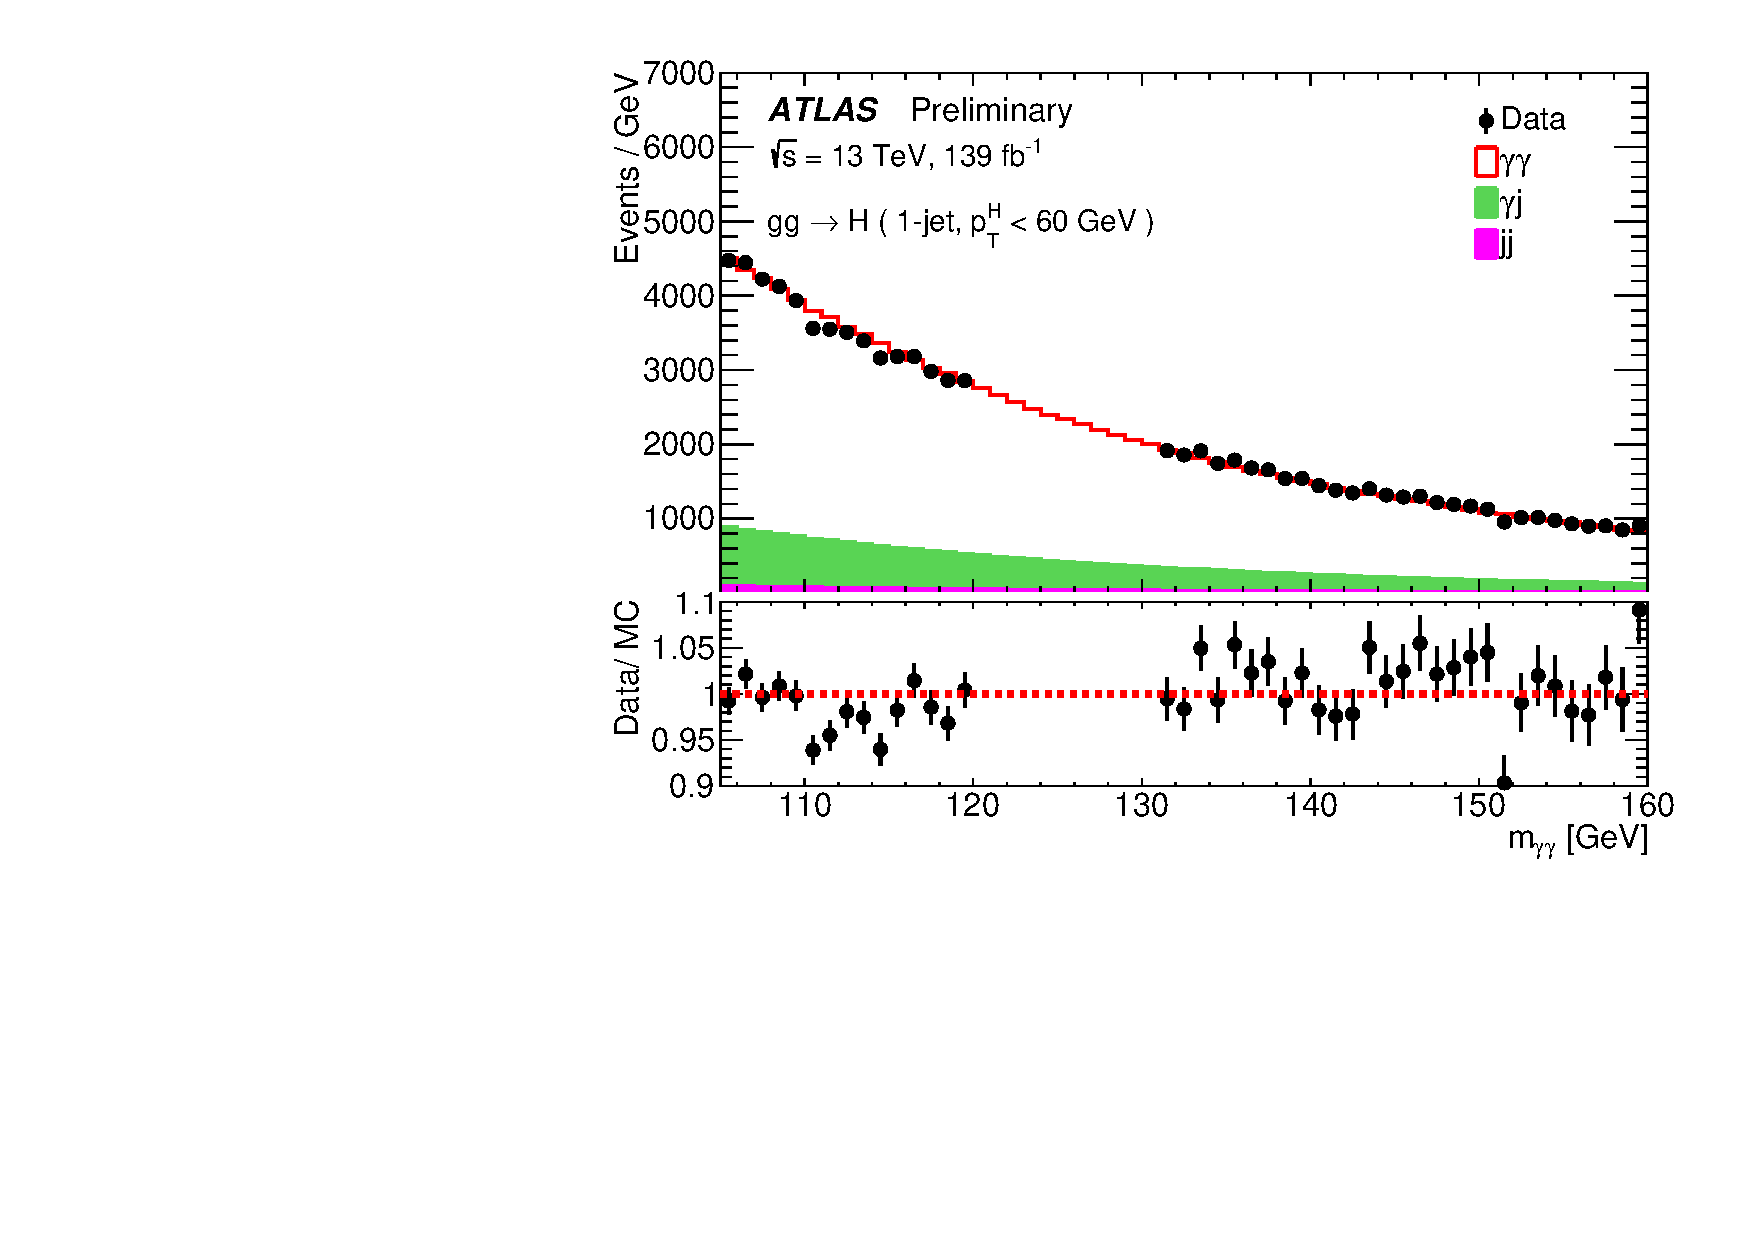
\includegraphics[width=0.49\textwidth]{figures/couplings_chapter/c2.pdf}\label{fig:design:bkg_ggH}}
\subfloat[\qqtoHqq\ ($\ge 2$-jets, $350 \le \mjj < 700\,\GeV$, $\ptH < 200\,\GeV$, $\ptHjj < 25\,\GeV$)]{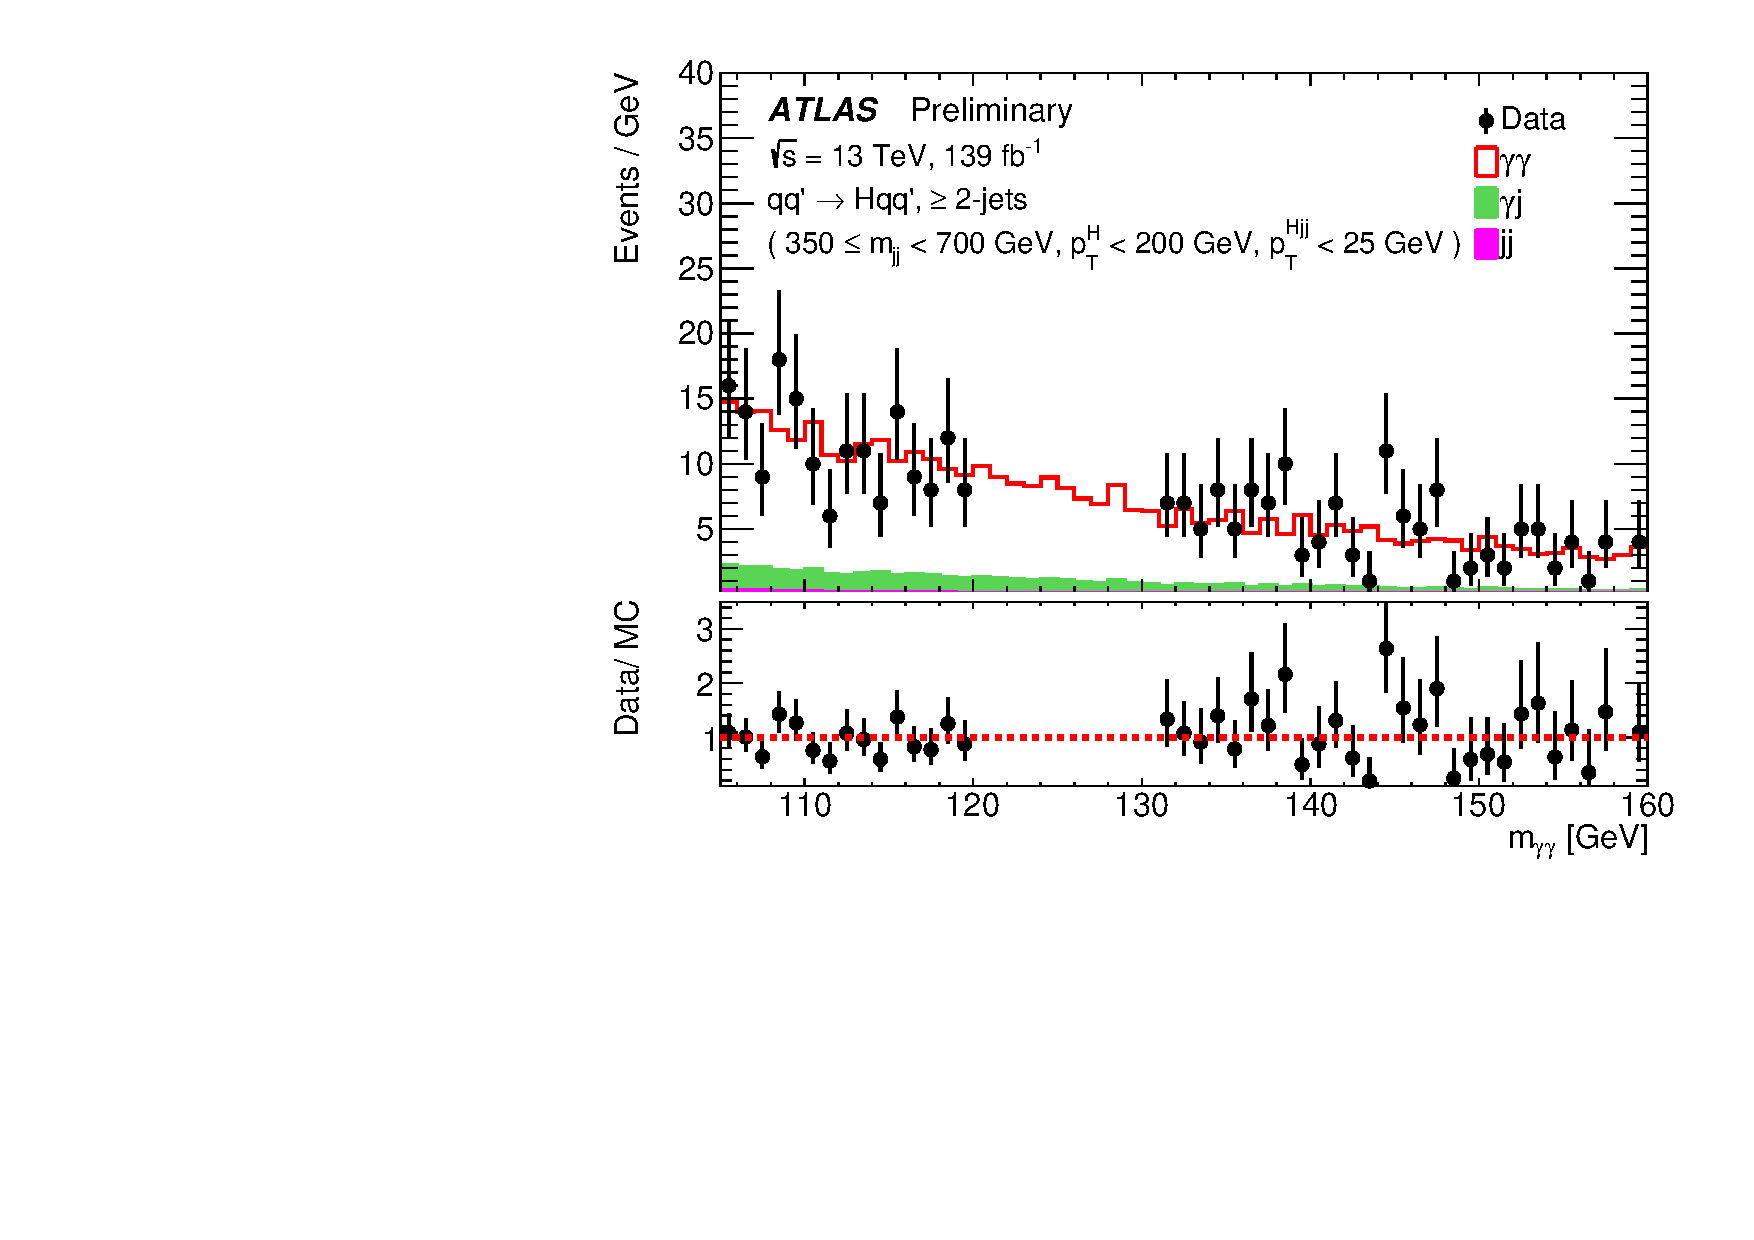
\includegraphics[width=0.49\textwidth]{figures/couplings_chapter/c52.pdf}\label{fig:design:bkg_VBF}}    \\
\subfloat[\qqtoHln\ ($75 \le \ptH < 150\,\GeV$)]{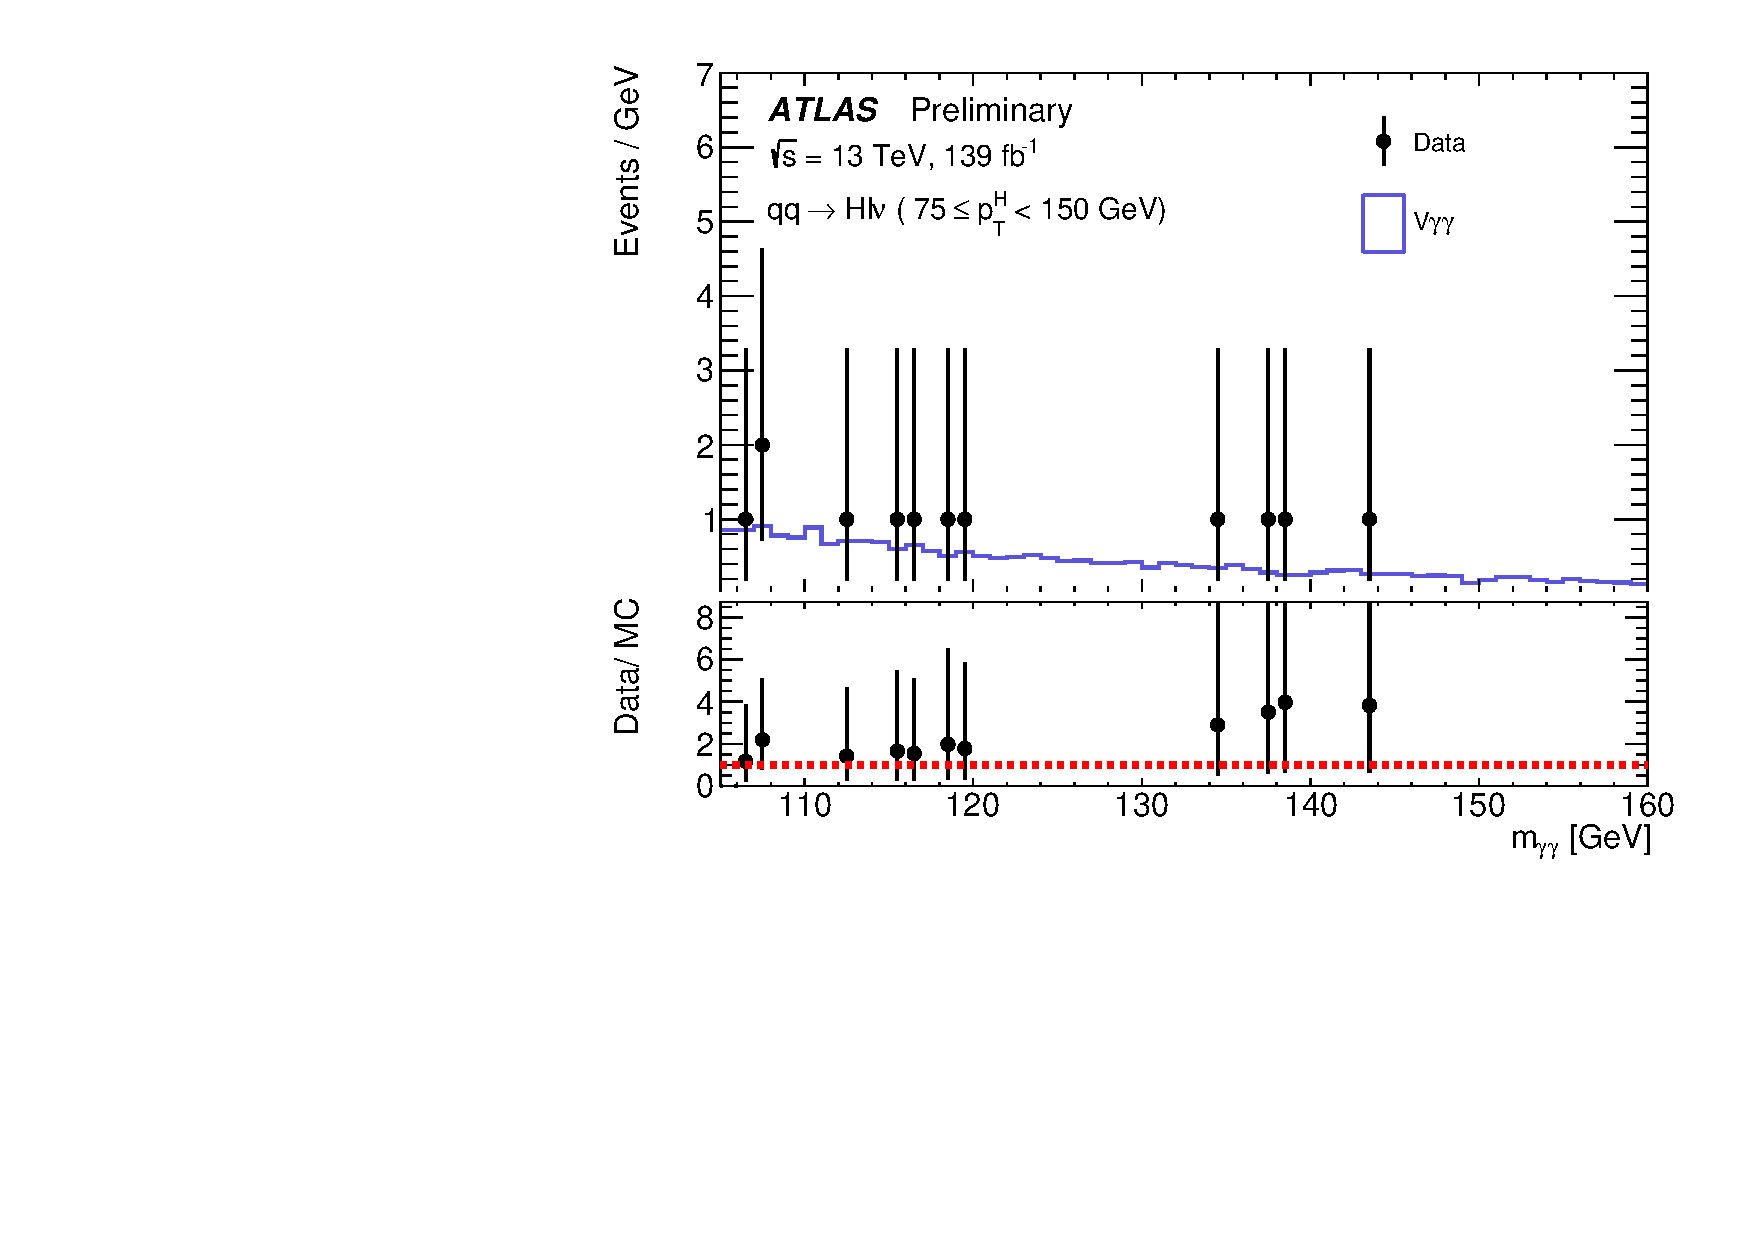
\includegraphics[width=0.49\textwidth]{figures/couplings_chapter/c67.pdf} \label{fig:design:bkg_VH}}
\subfloat[\ttH\ ($60 \le \ptH < 120\,\GeV$)]{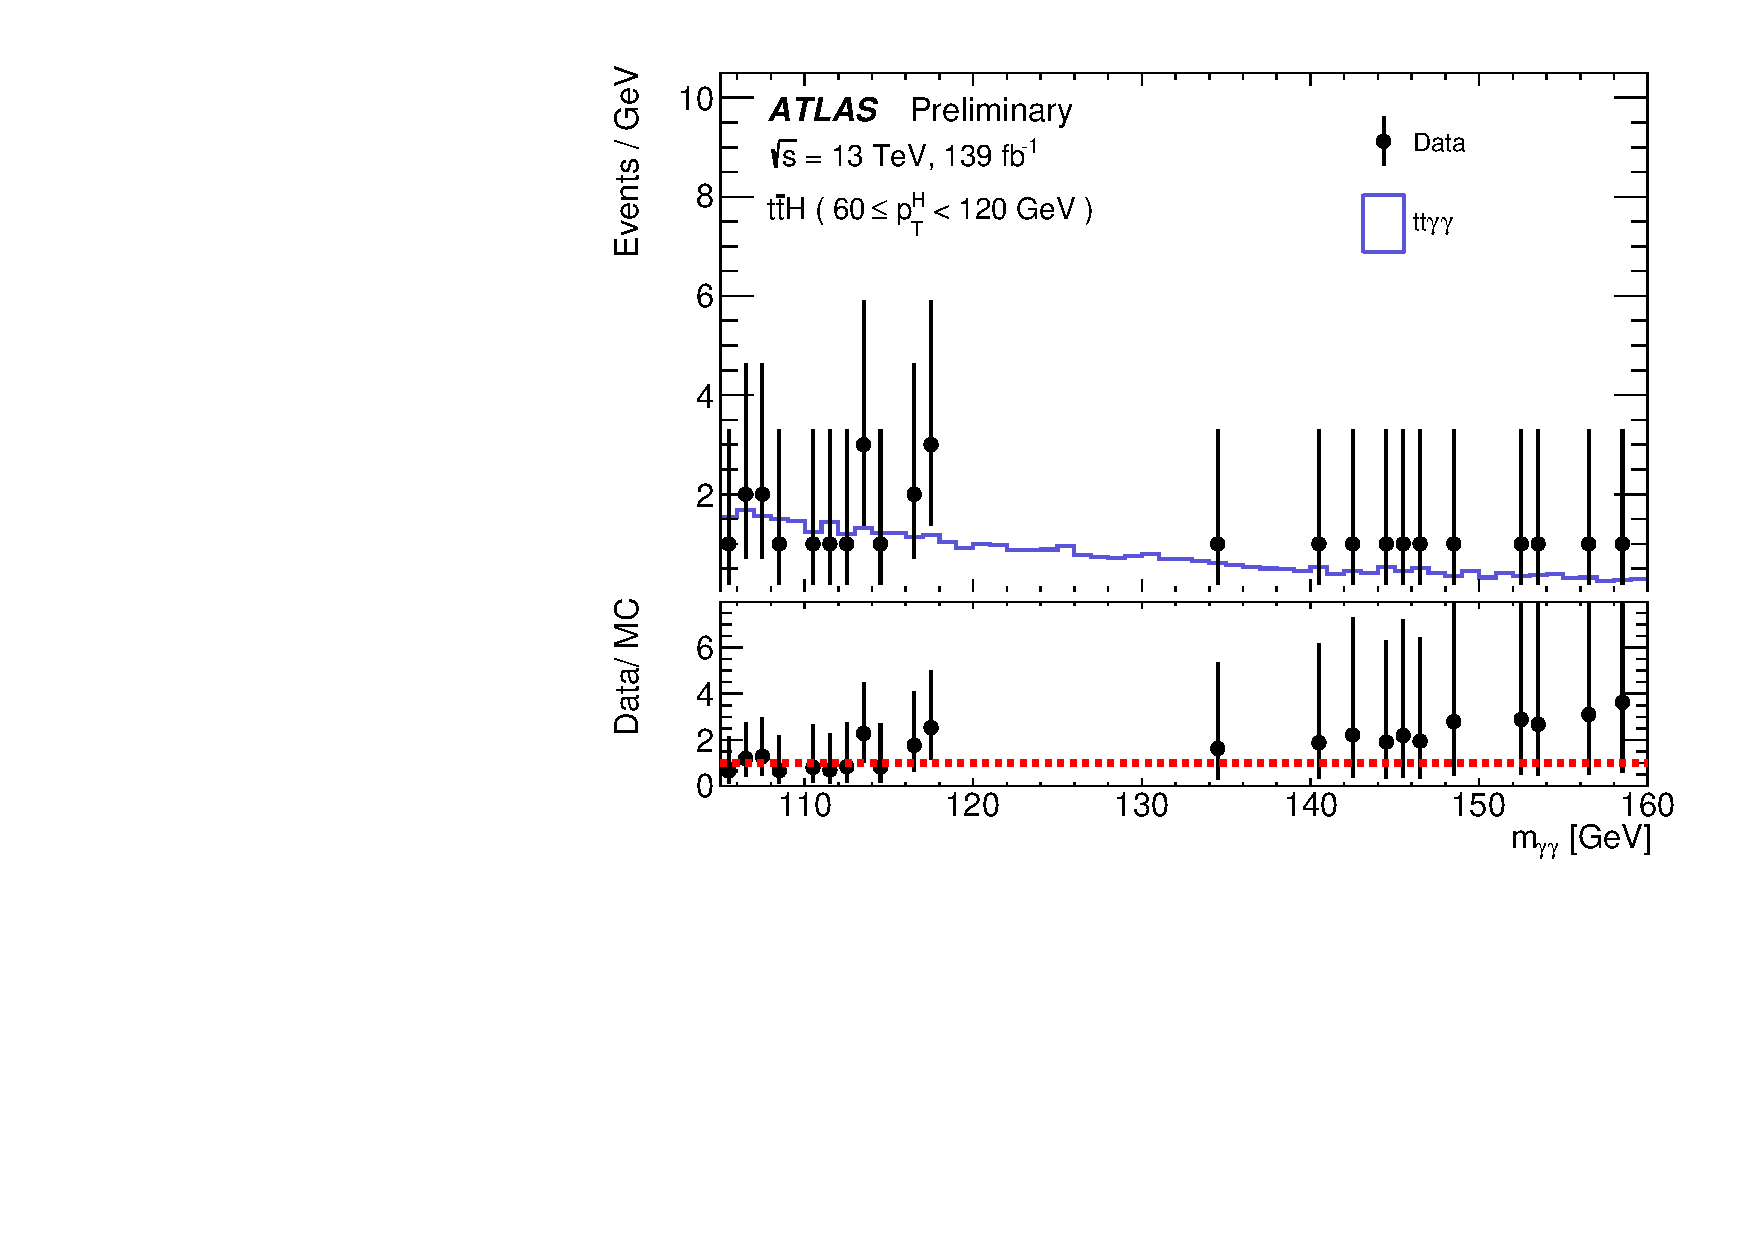
\includegraphics[width=0.49\textwidth]{figures/couplings_chapter/c80.pdf}\label{fig:design:bkg_ttH}}
\caption{Distribution of the diphoton invariant mass $m_{\gamma \gamma}$ in four STXS categories. Monte Carlo background templates are shown in histogram, and data is shown using black points. The signal region, $120 < m_{\gamma \gamma} < 130 \GeV$, is excluded in data. In categories~\ref{fig:design:bkg_ggH} and~\ref{fig:design:bkg_VBF}, the $\gamma \gamma$, $\gamma j$ (green) and $jj$ (magenta) components of the background used to build the template are shown stacked on top of each other. }
\label{fig:design:bkg}
\end{figure}

\section{Systematic Uncertainties} \label{sec:Systematics} 

Systematics follow a similar prescription as in the CP analysis. They can be broadly split up into two sources, experimental and theoretical, and can influence the overall yield and distribution shapes for different processes, or cause migration between STXS bins. 

Due to the large number of nuisance parameters, a nuisance parameter is removed from consideration if it has an effect of $< 0.3\%$ when varied up or down by one standard deviation.

\subsection{Theory Systematics} \label{subsec:Theorysysts}

Theory systematics can broadly be broken down into perturbative QCD scale uncertainties, PDF + $\alpha_{S}$ uncertainties, uncertainty on the $H \rightarrow \gamma \gamma$ branching ratio, QCD effects in the soft (low-energy) regime, and final state heavy-flavor jet uncertainty.

Because the $ggF$ process is being measured specifically in fine STXS bins and not being selected against as in the CP analysis, and because the final-state jet multiplicity may vary, it is not enough to simply vary the QCD renormalization and factorization scales to account for QCD effects in $ggF$, as in the CP analysis. Thus, for $ggF$, the QCD uncertainty is broken up into 14 individual nuisance parameters, including QCD resummation and factorization scale uncertainties, migration uncertainties across different jet-multiplicity regimes, and migration between STXS bins with differing values of $p_{T}^{Hjj}$ and $m_{jj}$. Additionally, a comparison of acceptance and efficiency factors between the nominal $ggF$ sample and the alternative MadGraph5\_aMC@NLO sample is made, and the differences are considered asadditional $ggF$ modeling uncertainties.

Additional QCD uncertainties on $VH$ processes are modelled, for similar reasons as for $ggH$: for each of $WH$, $qq/qg /rightarrow ZH$, and $gg \rightarrow ZH$, one source of overall yield uncertainty, four sources of $p_{T}^{V}$ modeling uncertainty, and two sources of jet multiplicity modeling uncertainty are accounted for. For $qq' \rightarrow H qq'$ processes, one uncertainty source is identified for overall yield variation, two for modeling of the jet multiplicity and $p_{T}^{Hjj}$ distributions, one for migration between $p_{T}^{H} < 200$ GeV and $p_{T}^{H} > 200$ GeV categories, and six for the modeling of the $m_{jj}$ distribution.

For $ttH$ and $tH$, one nuisance parameter is introduced for the yield and six are introduced for the $p_{T}^{H}$ distribution.

The value of the various QCD scale uncertainties varies between categories, but is found to have an effect of between 5\% and 25\%.

Parton showering uncertainty is evaluated by comparing the Pythia8 and Herwig7 Monte Carlo samples. Doing so leads to six nuisance parameters in each category; the effect of each of these is found to be approximately 10\% or less.

The PDF and $\alpha_{S}$ uncertainties are evaluated using the PDF4LHC15 \ref{cite:PDF4LHC15} prescription, using a matrix method designed to facilitate easier combination with other Higgs decay channels. Effects are typically very small compared to other sources of theory uncertainty.

As in the CP analysis, in categories targeting $ttH$ and $tH$, we apply a 100\% yield uncertainty on the $ggF$, $VBF$, and $VH$ processes, due to poor modelling of these processes in events containing final-state hadrons. This is supported by measurements in $H \rightarrow ZZ^{*}\rightarrow 4l$ \ref{cite:HZZ4l}, $t\bar{t}b\bar{b}$ \ref{cite:ttbb}, and $Vb$ \ref{cite:Vb}.

The theoretical uncertainties on the Higgs boson production cross section and the $H \rightarrow \gamma \gamma$ decay branching ratio are not used in the measurements. However, the $H \rightarrow \gamma \gamma$ decay branching ratio has an uncertainty of 1.6\%, according to the HDECAY and PROPHECY4F programs.

The largest theoretical systematic is the parton showering and underlying event modelling, and its impact on the measured cross sections can be up to 11\% in some $VBF$ categories. 

\subsection{Experimental Systematics} \label{subsec:Experimentalsysts}

Experimental systematics can broadly be broken up into two categories, those influencing or resulting from the shape of functional forms used in the fit (photon energy scale, photon energy resolution) and those influencing the overall yield (due to object reconstruction effects, luminosity, Higgs mass mismeasurement, and pileup reweighting).

The photon energy scale and resolution are included as response functions on $\mu_{CB}$ and $\sigma_{CB}$, respectively. They are extracted for each individual category from Monte Carlo samples with these parameters varied and are treated as uncorrelated variations across categories. For the photon energy scale, the nominal mean is compared with that of the varied sample, while for the photon energy resolution, the inter-quartile range is compared across samples. A fully-decorrelated model is used for photon energy resolution and a merged scheme is used for photon energy scale, due to the minimal sensitivity of the analysis to scale variations. Scale uncertainties are treated with a Gaussian constraint, while resolution uncertainties are treated with asymmetric constraints. Their impact is between 1\% and 8\%, depending on the category.

85 additional nuisance parameters are introduced to model yield variations. These include jet reconstruction uncertainties such as jet flavor composition, flavor response, jet modelling, jet topology, and jet energy resolution \ref{cite:coups127} as well as b-tagging efficiency \ref{cite:coups130}. Photon isolation and identification efficiency uncertainties \ref{cite:coups116}, spurious signal, trigger efficiency \ref{cite:coups27}, and luminosity uncertainty (obtained using the LUCID-2 detector) \ref{cite:LUCID} are also parameterized in this way. These systematics are treated as correlated, and are treated with either asymmetric or log-normal constraints.

Spurious signal uncertainty ranges from 10\% to 99\% of the statistical uncertainty in categories, depending on statistics. It is considered to be uncorrelated across categories.

Pileup uncertainty is modelled by varying the cross-section used to reweight pileup interactions from Monte Carlo to the data up or down by 9\%. 

For $ggH$ and $VH$ categories, the leading experimental systematic uncertainty arises from the spurious signal, with an impact of around 4\% on the cross-section. For the $VBF$ and $ttH+tH$, the leading experimental uncertainty is jet modelling, and with an impact that can rise to as large as 6\%.

The impact of all systematics in the five-production-mode fit (combining STXS bins) is given in Table \label{tab:result:systematic}. 

\begin{table}[!htp]
\begin{center}
\resizebox{0.995\textwidth}{!}{
\begin{tabular}{llllllllllll}
\hline
 & \ggF+~\bbH & \VBF & \WH & \ZH & \ttH+~\tH \\
\hline
Uncertainty source & $\Delta\sigma$[\%] & $\Delta\sigma$[\%] & $\Delta\sigma$[\%] & $\Delta\sigma$[\%] & $\Delta\sigma$[\%] \\
\hline
\hline
\hspace{3mm}Underlying Event and Parton Shower (UEPS)  & $\pm$2.3 & $\pm$10 & $<\pm$1 & $\pm$9.6 & $\pm$3.5 \\
\hspace{3mm}Modeling of Heavy Flavor Jets in non-$t\bar{t}H$ Processes & $<\pm$1 & $<\pm$1 & $<\pm$1 & $<\pm$1 & $\pm$1.3 \\
\hspace{3mm}Higher-Order QCD Terms (QCD)  & $\pm$1.6 & $<\pm$1 & $<\pm$1 & $\pm$1.9 & $<\pm$1 \\
\hspace{3mm}Parton Distribution Function and $\alpha_S$ Scale (PDF+$\alpha_S$) & $<\pm$1 & $\pm$1.1 & $<\pm$1 & $\pm$1.9 & $<\pm$1 \\
\hspace{3mm}Photon Energy Resolution (PER)   & $\pm$2.9 & $\pm$2.4 & $\pm$2.0 & $\pm$1.3 & $\pm$4.9 \\
\hspace{3mm}Photon Energy Scale (PES)  & $<\pm$1 & $<\pm$1 & $<\pm$1 & $\pm$3.4 & $\pm$2.2 \\
\hspace{3mm}Jet/\MET & $\pm$1.6 & $\pm$5.5 & $\pm$1.2 & $\pm$4.0 & $\pm$3.0 \\
\hspace{3mm}Photon Efficiency & $\pm$2.5 & $\pm$2.3 & $\pm$2.4 & $\pm$1.4 & $\pm$2.4 \\
\hspace{3mm}Background Modeling & $\pm$4.1 & $\pm$4.7 & $\pm$2.8 & $\pm$18 & $\pm$2.4 \\
\hspace{3mm}Flavor Tagging & $<\pm$1 & $<\pm$1 & $<\pm$1 & $<\pm$1 & $<\pm$1 \\
\hspace{3mm}Leptons  & $<\pm$1 & $<\pm$1 & $<\pm$1 & $<\pm$1 & $<\pm$1 \\
\hspace{3mm}Pileup  & $\pm$1.8 & $\pm$2.7 & $\pm$2.1 & $\pm$3.8 & $\pm$1.1 \\
\hspace{3mm}Luminosity and Trigger   &  $\pm$2.1 & $\pm$2.1 & $\pm$2.3 & $\pm$1.1 & $\pm$2.3 \\
\hspace{3mm}Higgs Boson Mass &  $<\pm$1 & $<\pm$1 & $<\pm$1 & $\pm$3.7 & $\pm$1.9 \\
\hline
\hline
\end{tabular}
}
  \caption{The impact of groups of systematic uncertainties on the total error on the measured cross section times branching ratio. This is shown as the uncertainty due to each group of uncertainties ($\Delta \sigma$), as a fraction of the total measured cross section ($\sigma$).}
\label{tab:result:systematic}
\end{center}
\end{table}

\section{Results} \label{sec:Results}

Three primary results are reported: First, an overall production cross-section; second, cross-sections for each of the five main individual production modes ($ggF+bbH$, $VBF$, $WH$, $ZH$, and $ttH+tH$); and third, cross-sections in each of the STXS bins. At the time of this writing, further work is being performed in order to prepare additional results that will interpret these cross-sections in terms of both the Kappa-Framework and in terms of constraints on Effective Field Theory (EFT) observables.

\subsection{Cross-Sections} \label{sec:Xsecs}

The overall cross-section is measured by profiling a single parameter, the cross-section times branching ratio ($\sigma \times B_{\gamma \gamma}$), which scales with the yield in each category. All 88 categories are fit simultaneously. The requirement $|y_{H}|<2.5$ is applied on both the 

Figure \ref{fig:result:inclusivemgg} shoes the $m_{\gamma\gamma}$ distribution across categories, weighted by the ratio $ln(1+\frac{S}{B})$ where S and B are the signal and background yields in the smallest $m_{\gamma\gamma}$ window measured to contain 90\% of signal events. The choice of this weight is designed to illustrate the impact of more signal-dominated categories in a manner similar to how they enter into the likelihood fit. 
The overall cross-section is measured to be:

\begin{equation}
(\sigma \times B_{\gamma \gamma})_{obs} =127 \pm 10 fb=127 \pm 7(stat.) \pm 7(syst.)fb
\end{equation}

with an expectation measured using post-fit Asimov data of:

\begin{equation}
(\sigma \times B_{\gamma \gamma})_{exp} =115 \pm 5 fb
\end{equation}

For the five-production mode model, $(\sigma \times B_{\gamma \gamma})$ is measured separately for each production mode: $ggF+bbH$, $VBF$, $ZH$, $WH$, and $ttH+tH$. The $m_{\gamma\gamma}$ distribution in these categories, weighted by the ratio $ln(1+\frac{S}{B})$, are shown in Figure \ref{fig:results:prodXS_spectra}. The measured cross-sections times the diphoton branching ratio are depicted in Table \ref{tab:results:prodXS} and Figure \ref{fig:results:prodXS}. The correlations between categories are depicted in Figure \ref{fig:results:prodXS_corr}. The observed (expected) significance values for the $VBF$, $WH$, and $ttH+tH$ processes are 7.5 (6.1) $\sigma$, 5.6 (2.8) $\sigma$, and 4.7 (5.0) $\sigma$, respectively. The expected significance for the $ZH$ process is 1.7 $\sigma$; however, no excess over the background is observed. Together, these correspond to a roughly 1.9 $\sigma$ deviation from the SM.

A possible source of this discrepancy is the strong anticorrelation observed between the $WH$ and $ZH$ processes: if these are combined into one $VH$ production mode, the cross-section becomes $(\sigma_{VH})_{obs} = 5.9 \pm 1.4fb = 5.9 \pm 1.4(stat.) \pm 0.4(syst.)fb$ compared to the SM expectation of $(\sigma_{VH})_{exp}=4.53 \pm 0.12fb$. This corresponds to no excess with respect to the SM result.

The anticorrelation is because the leptonic $ZH$ categories suffer from substantial $WH$ contamination and an excess is observed in the leptonic $WH$ categories, so when $\mu_{WH}$ is higher, in order to converge, the fit must overestimate the contribution of $WH$ and underestimate the contribution of $ZH$. In order to rectify this, at the time of this writing, a new categorization scheme is being devised that will introduce a high-purity leptonic $ZH$ region by splitting on lepton multiplicity that should help this to decorrelate further.

A limit is also placed on the $tH$ cross-section using the $CL_{s}$ method (\ref{cite:CLs}). The limit is found to be 8.2 times the Standard Model expectation, stronger than the limit placed in the CP analysis. 


\begin{figure}
    \centering
    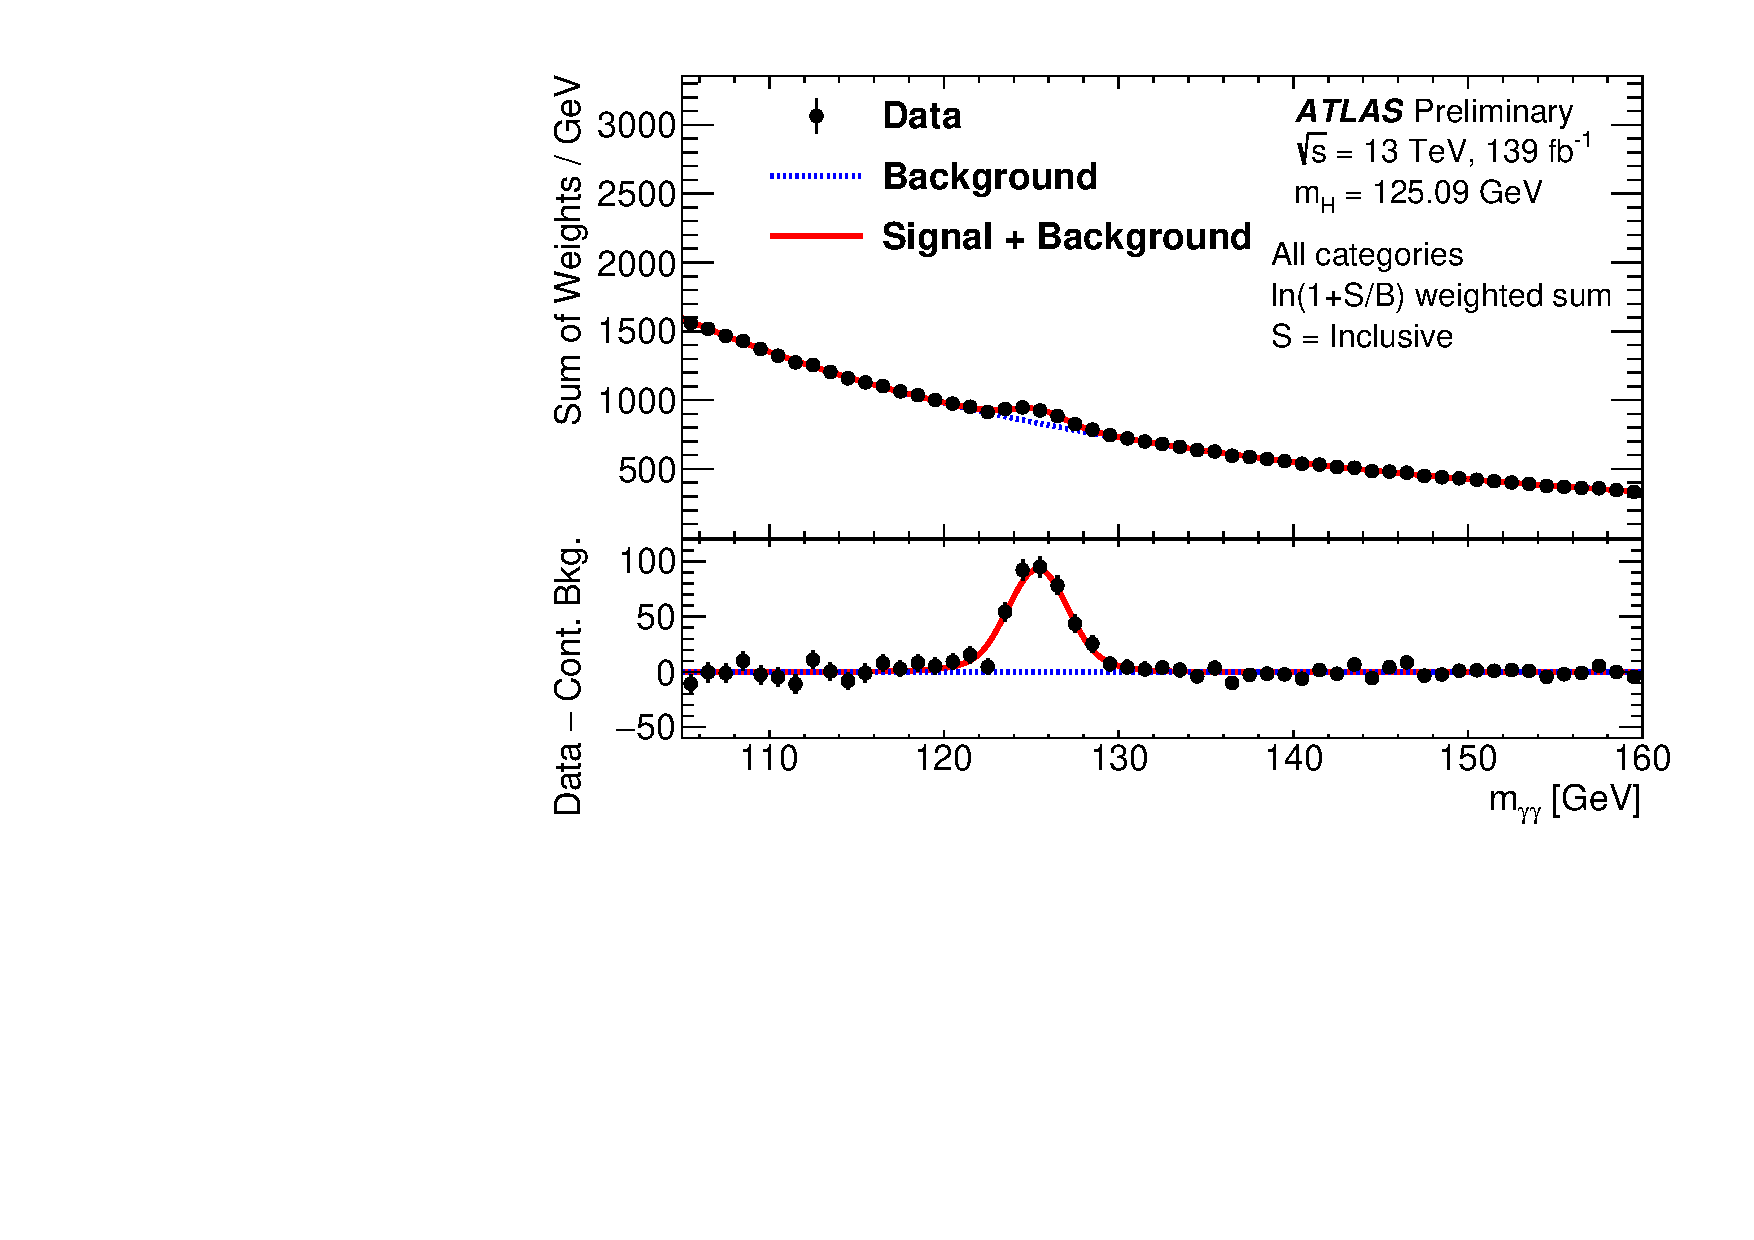
\includegraphics[width=0.8\textwidth]{figures/couplings_chapter/weighted_coupling2020_all.pdf}
    \caption{The inclusive diphoton invariant mass distribution of events from all analysis categories. The events in each category are weighted by $\ln(1+S/B)$, where $S$ and $B$ are the expected signal and background yields in this category within the smallest $m_{\gamma \gamma}$ window containing 90\% of the signal events. The weighted sum of the signal plus background fits is represented by the solid line, while the blue dotted line indicates the weighted sum of the background functional forms. }
    \label{fig:result:inclusivemgg}
\end{figure}

\begin{figure}[tpb!]
\centering
\subfloat[\ggF+~\bbH]{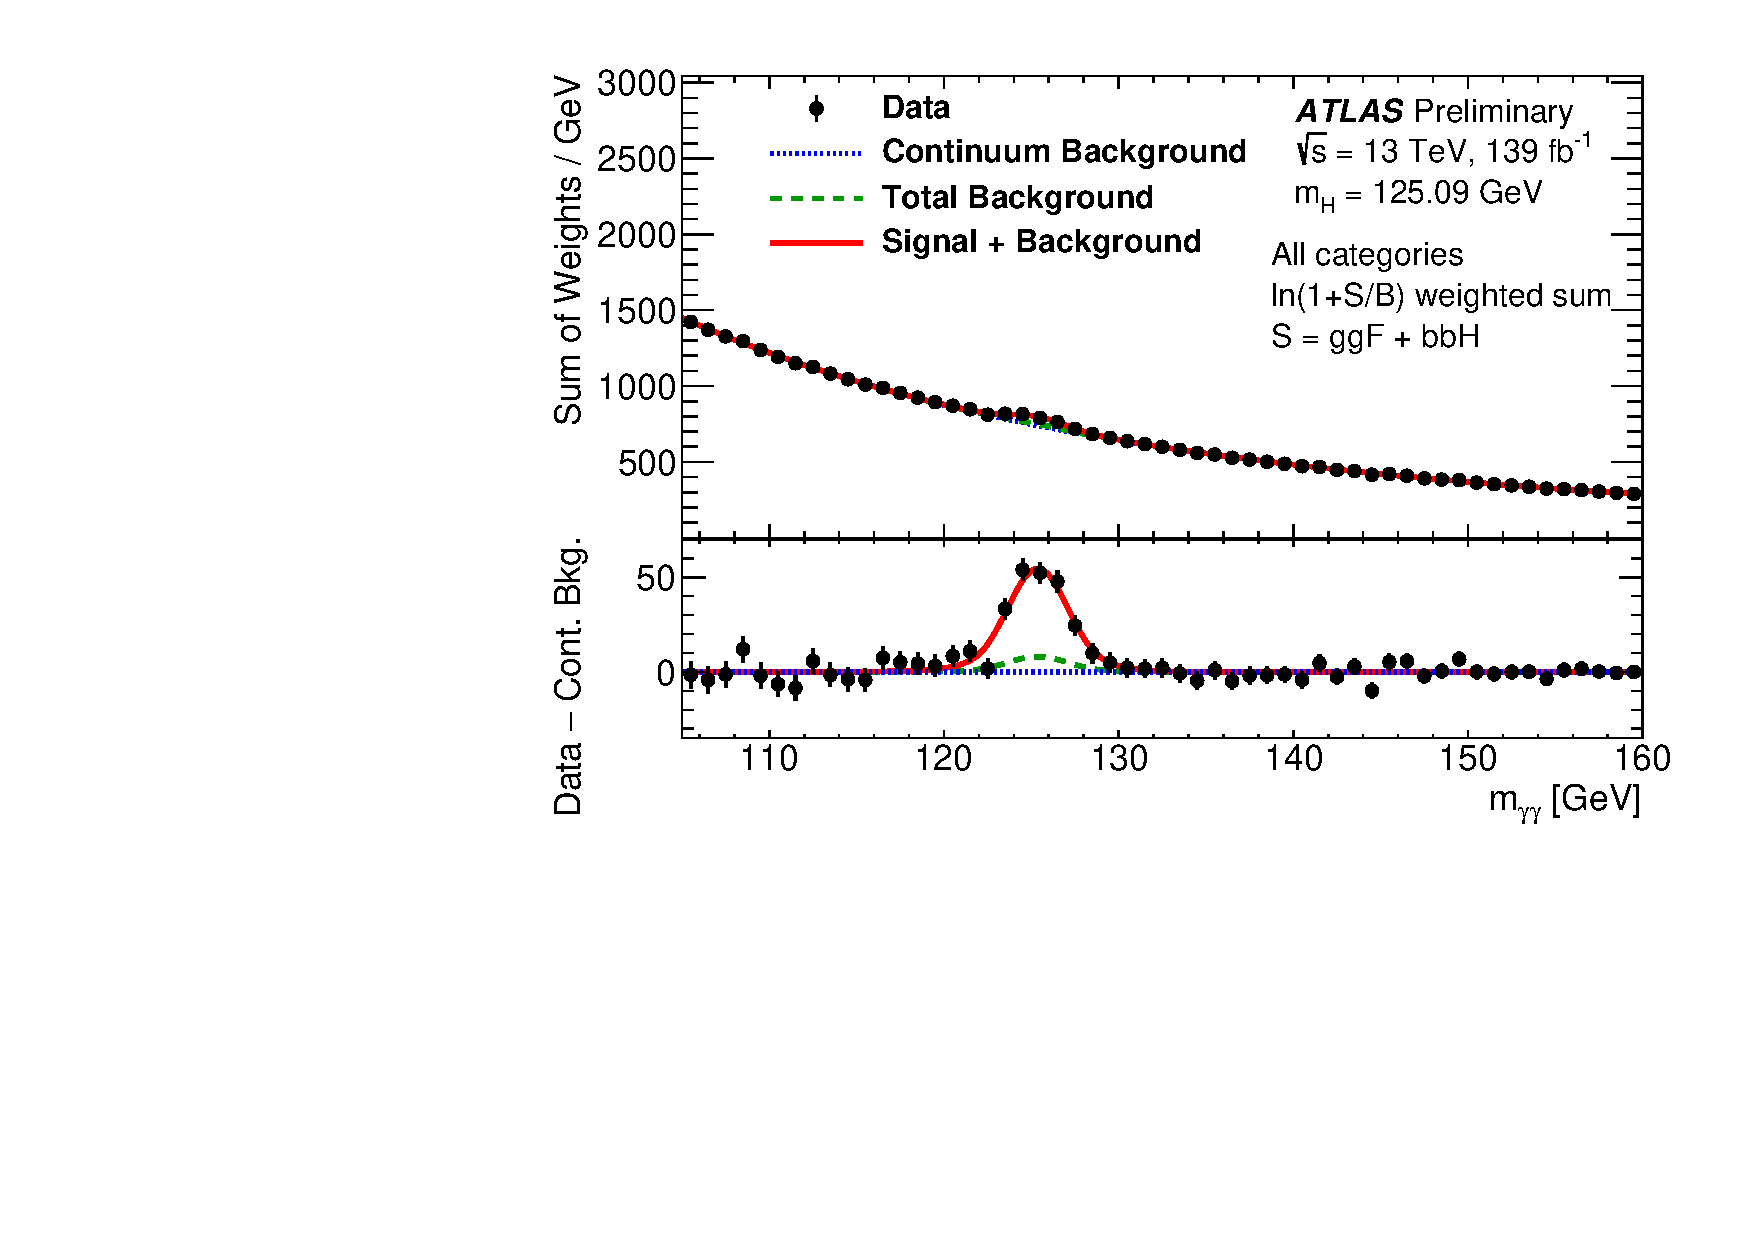
\includegraphics[width=.475\textwidth]{figures/couplings_chapter/weighted_coupling2020_all_ggF.pdf}}
\subfloat[\VBF]{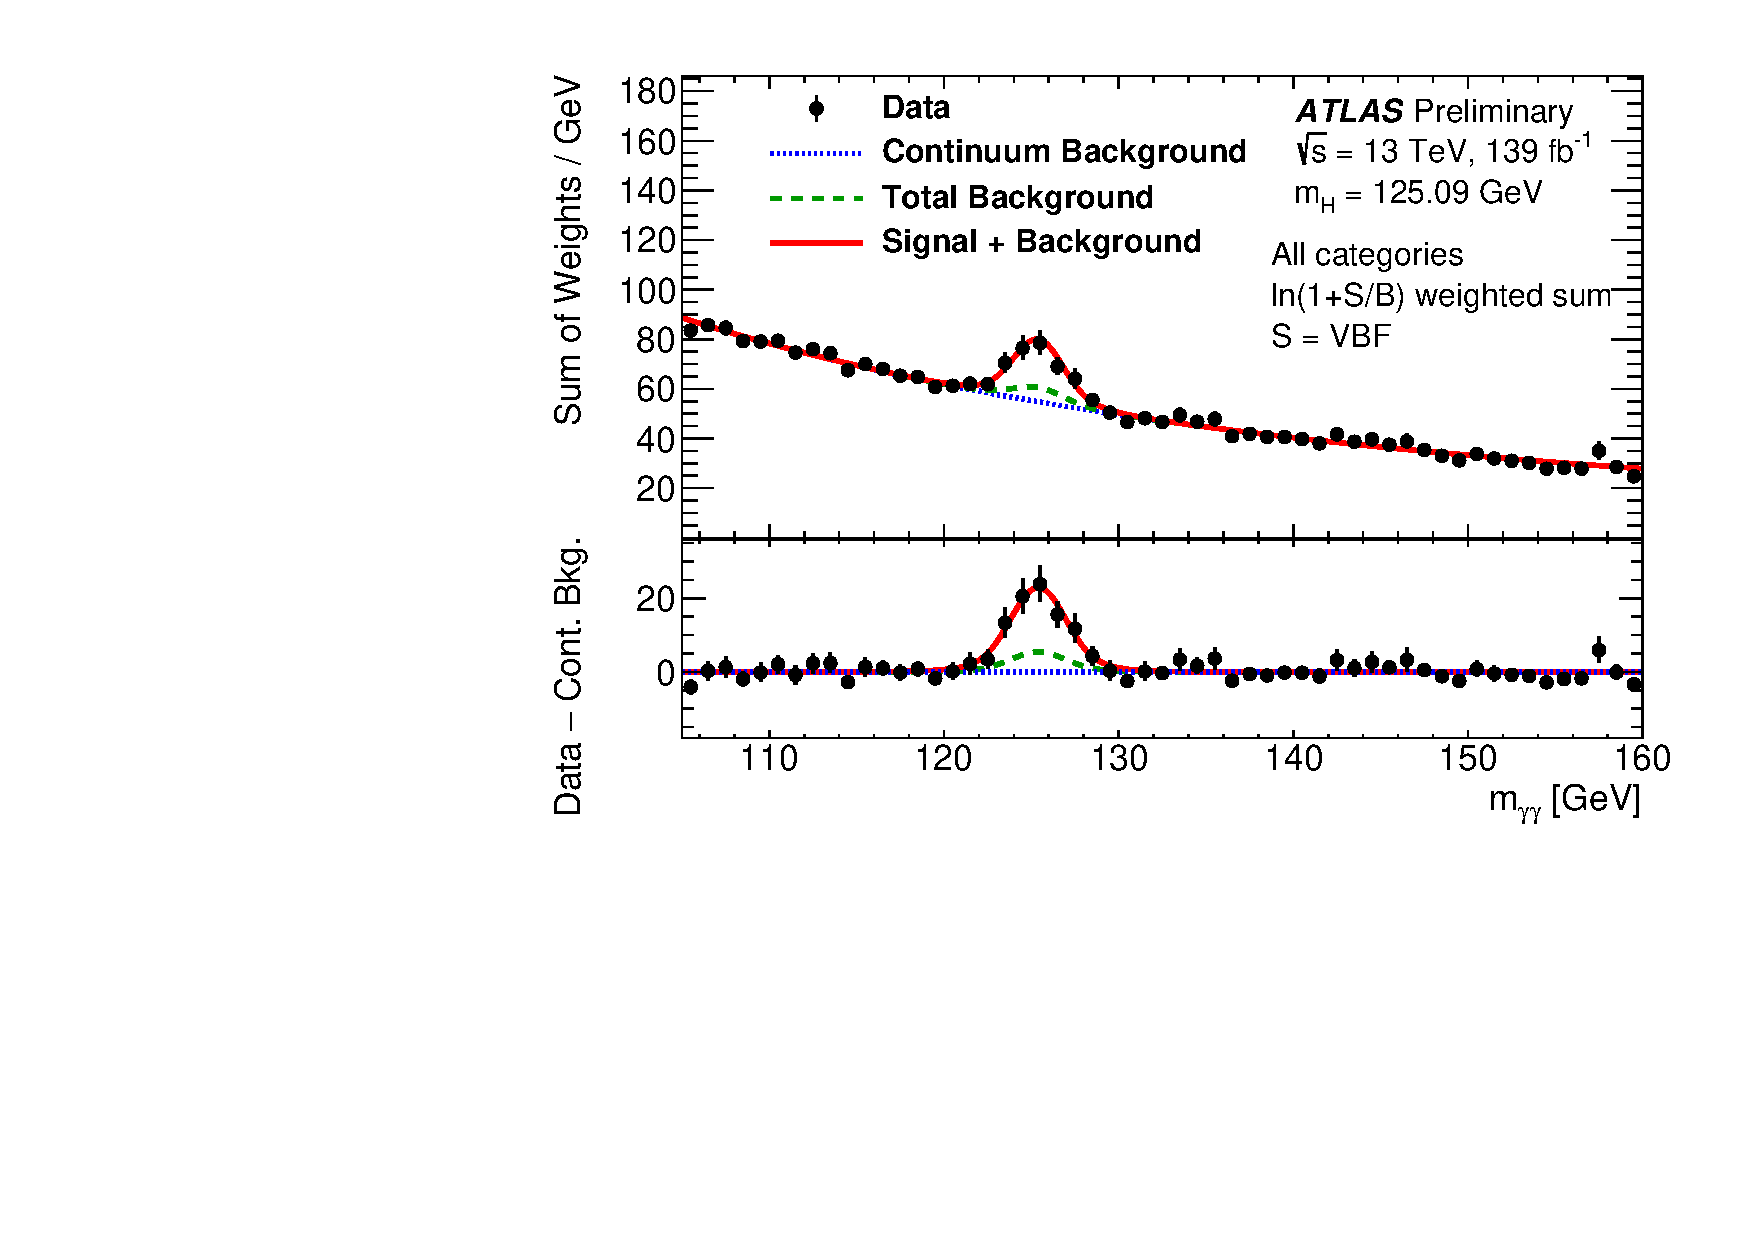
\includegraphics[width=.475\textwidth]{figures/couplings_chapter/weighted_coupling2020_all_VBF.pdf} }\\
\subfloat[\WH]{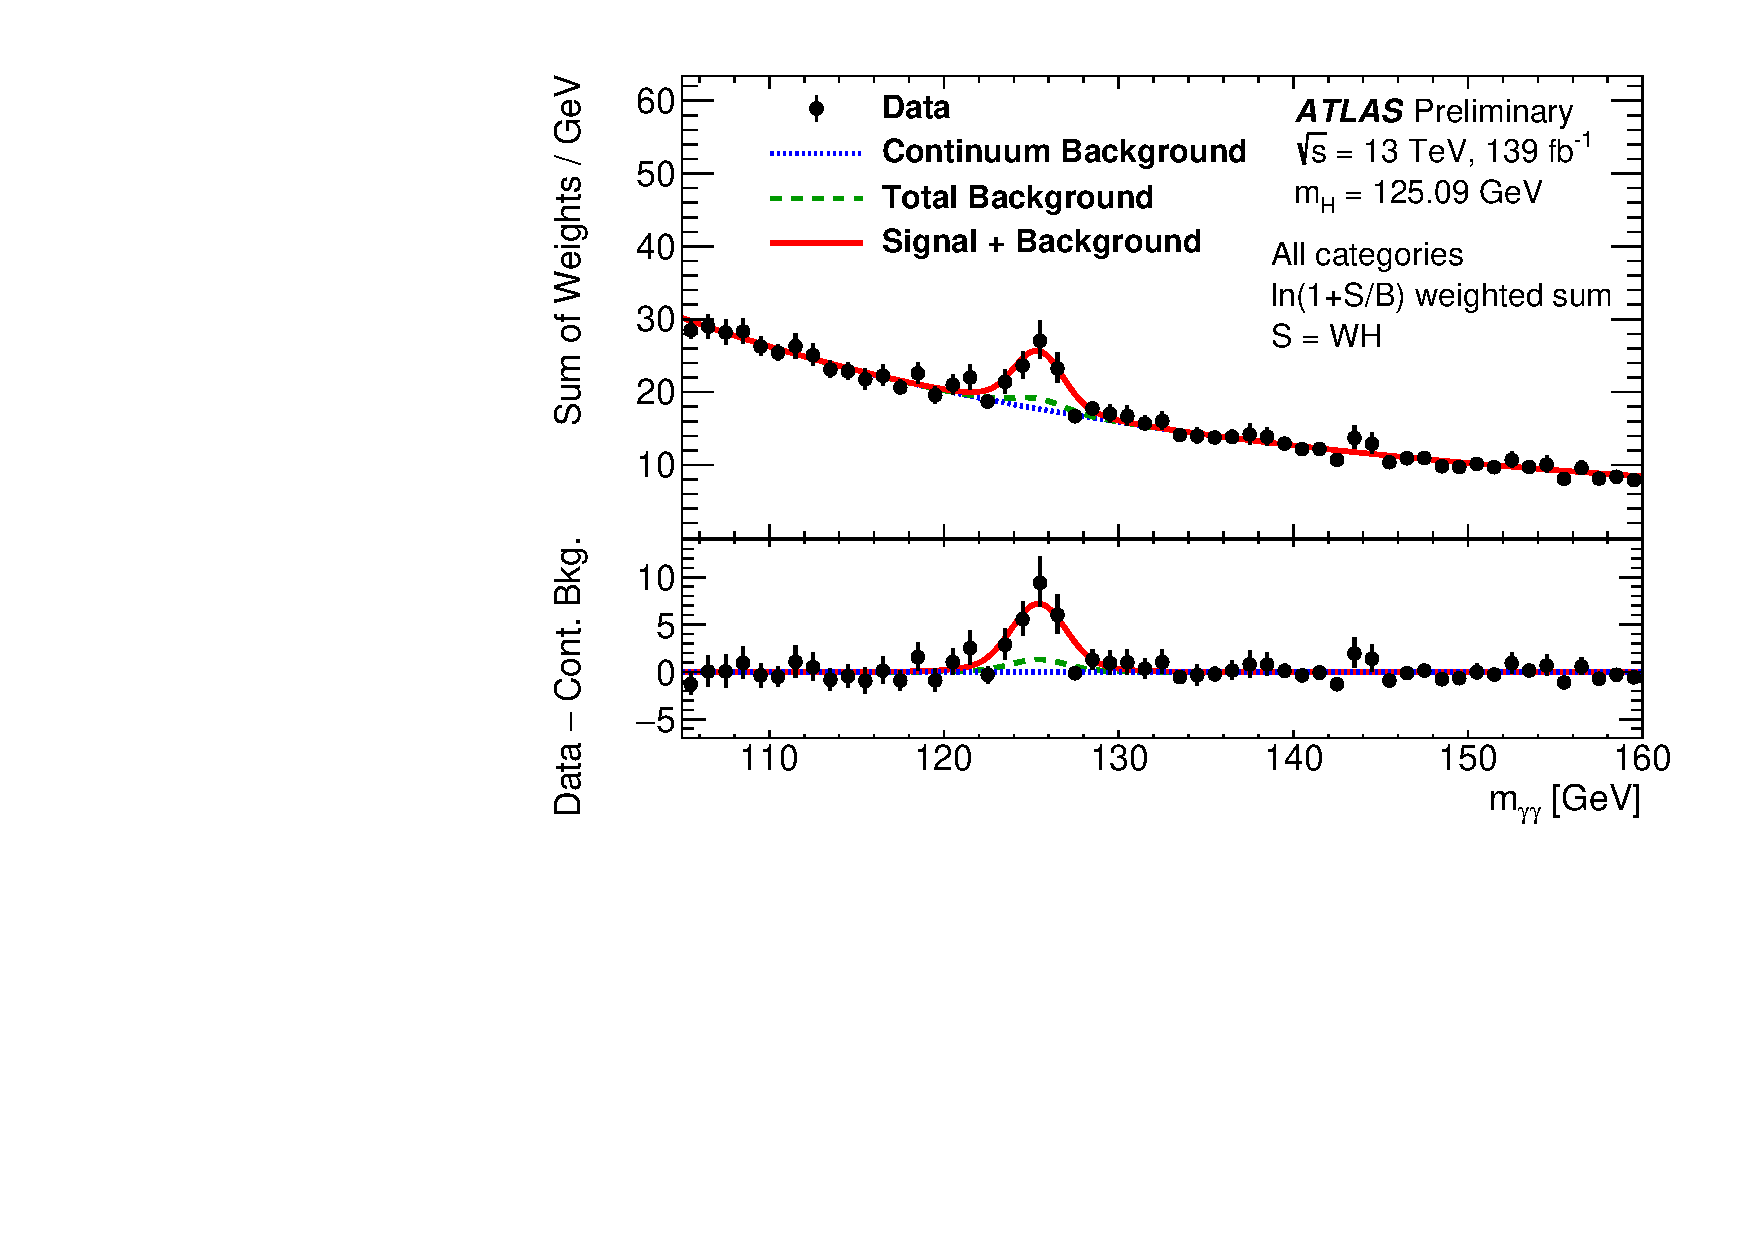
\includegraphics[width=.475\textwidth]{figures/couplings_chapter/weighted_coupling2020_all_WH.pdf}}
\subfloat[\ZH]{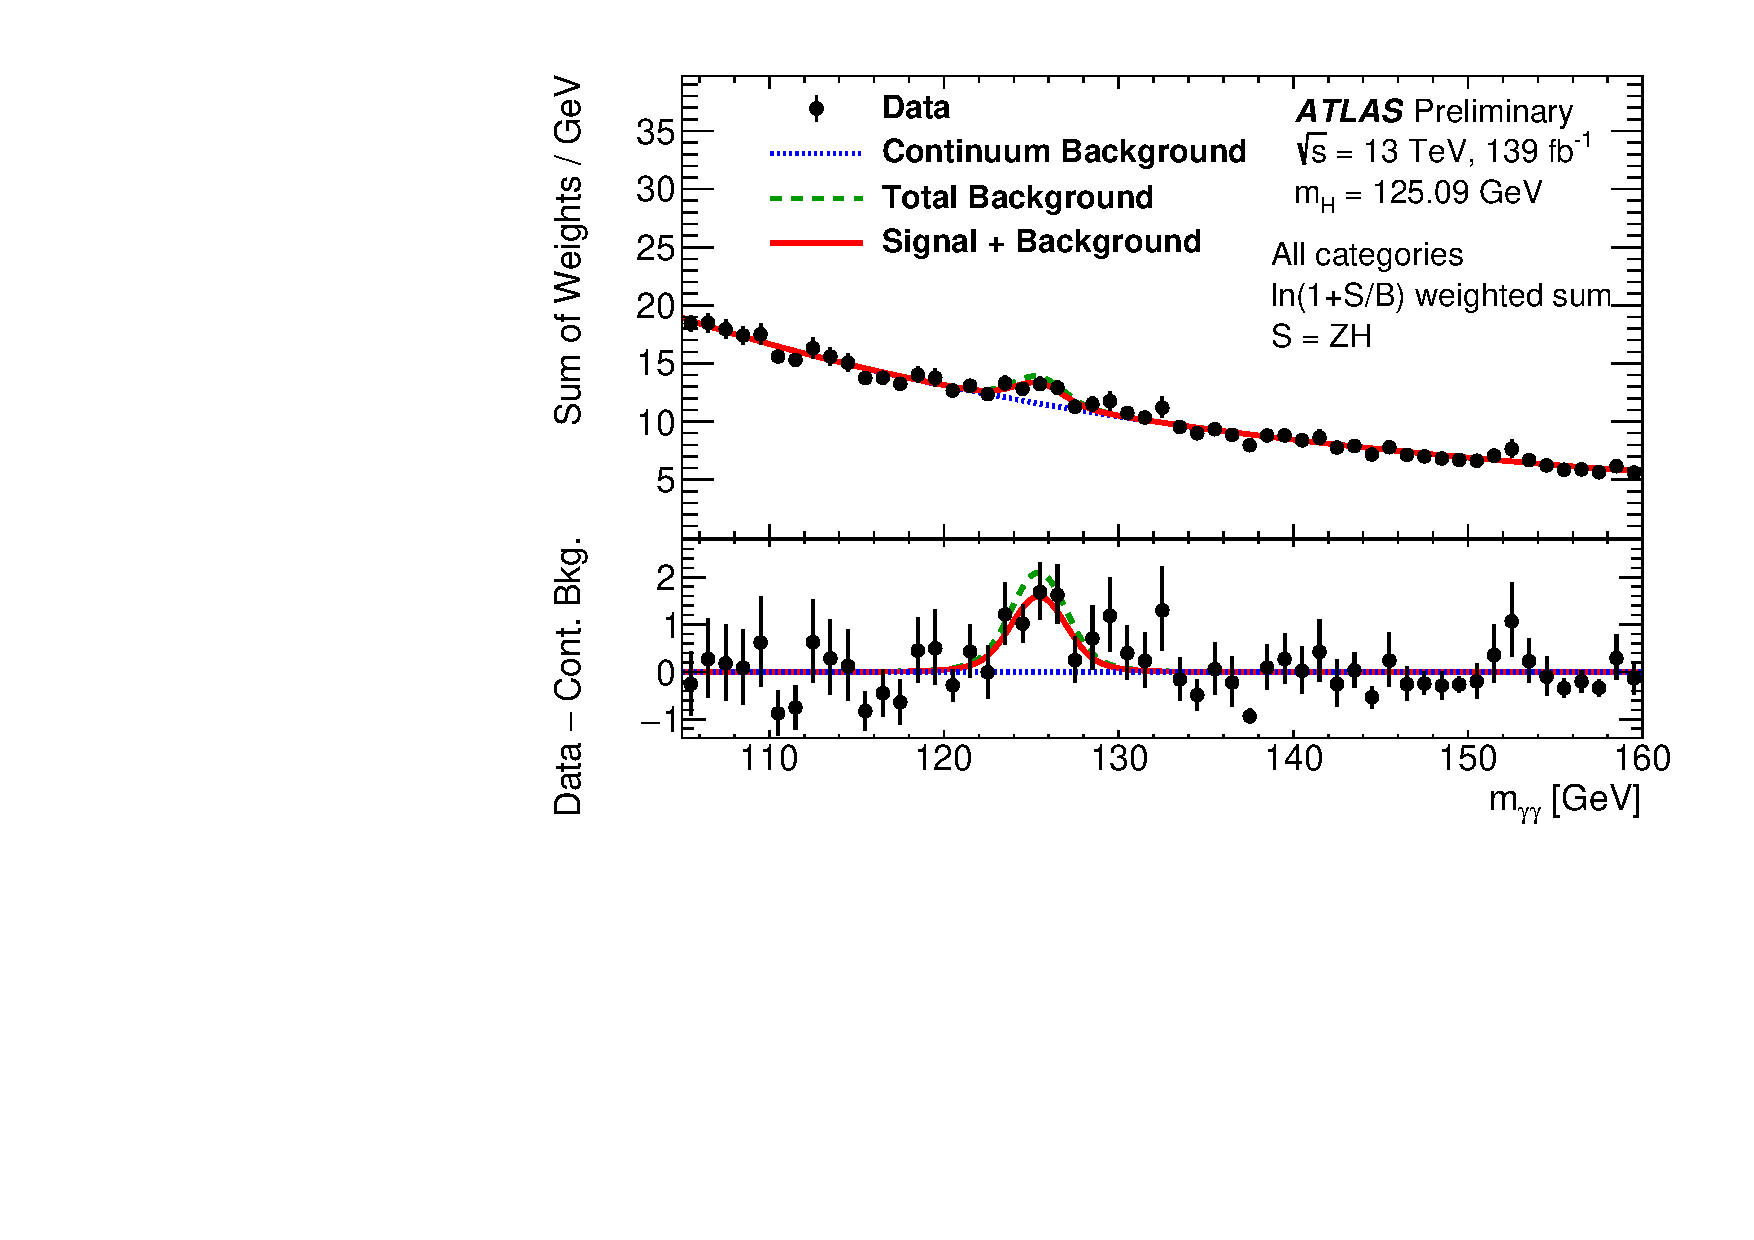
\includegraphics[width=.475\textwidth]{figures/couplings_chapter/weighted_coupling2020_all_ZH.pdf}}\\
\subfloat[\ttH+~\tH]{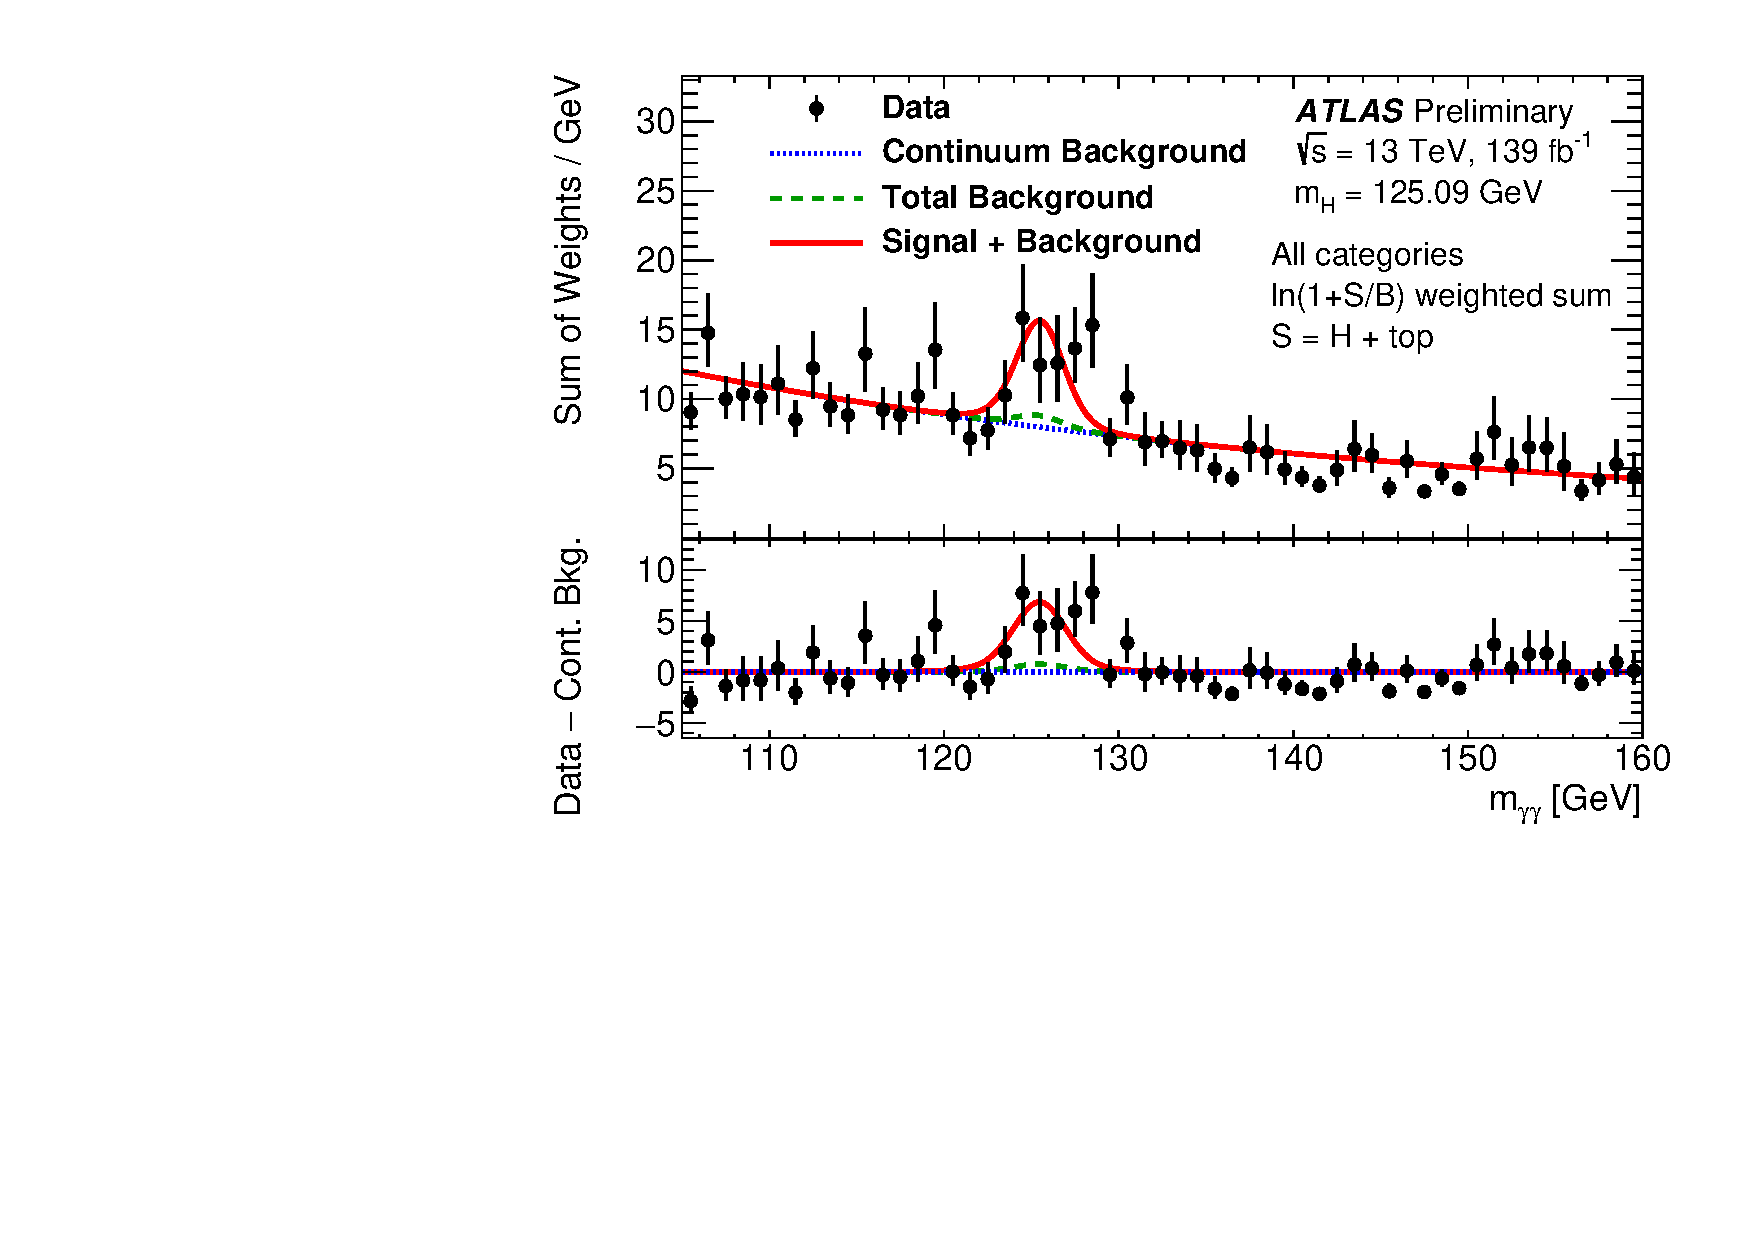
\includegraphics[width=.475\textwidth]{figures/couplings_chapter/weighted_coupling2020_all_ttHtH.pdf}}
\caption{Combined diphoton invariant mass distributions for the five-production-mode fit. The events in each category are weighted by $\ln(1+S/B)$, where $S$ and $B$ are the expected signal and background yields in this category within the smallest $m_{\gamma \gamma}$ window containing 90\% of the signal events. The weighted sum of the signal plus background fits is represented by the solid line, while the blue dotted line represents the weighted sum of the background functional forms. Only Higgs boson events from the targeted production processes in each category are considered as signal events in these plots; Higgs boson events from other processes are treated as part of the background.}
\label{fig:results:prodXS_spectra}
\end{figure}

\begin{figure}[h!]
  \centering
  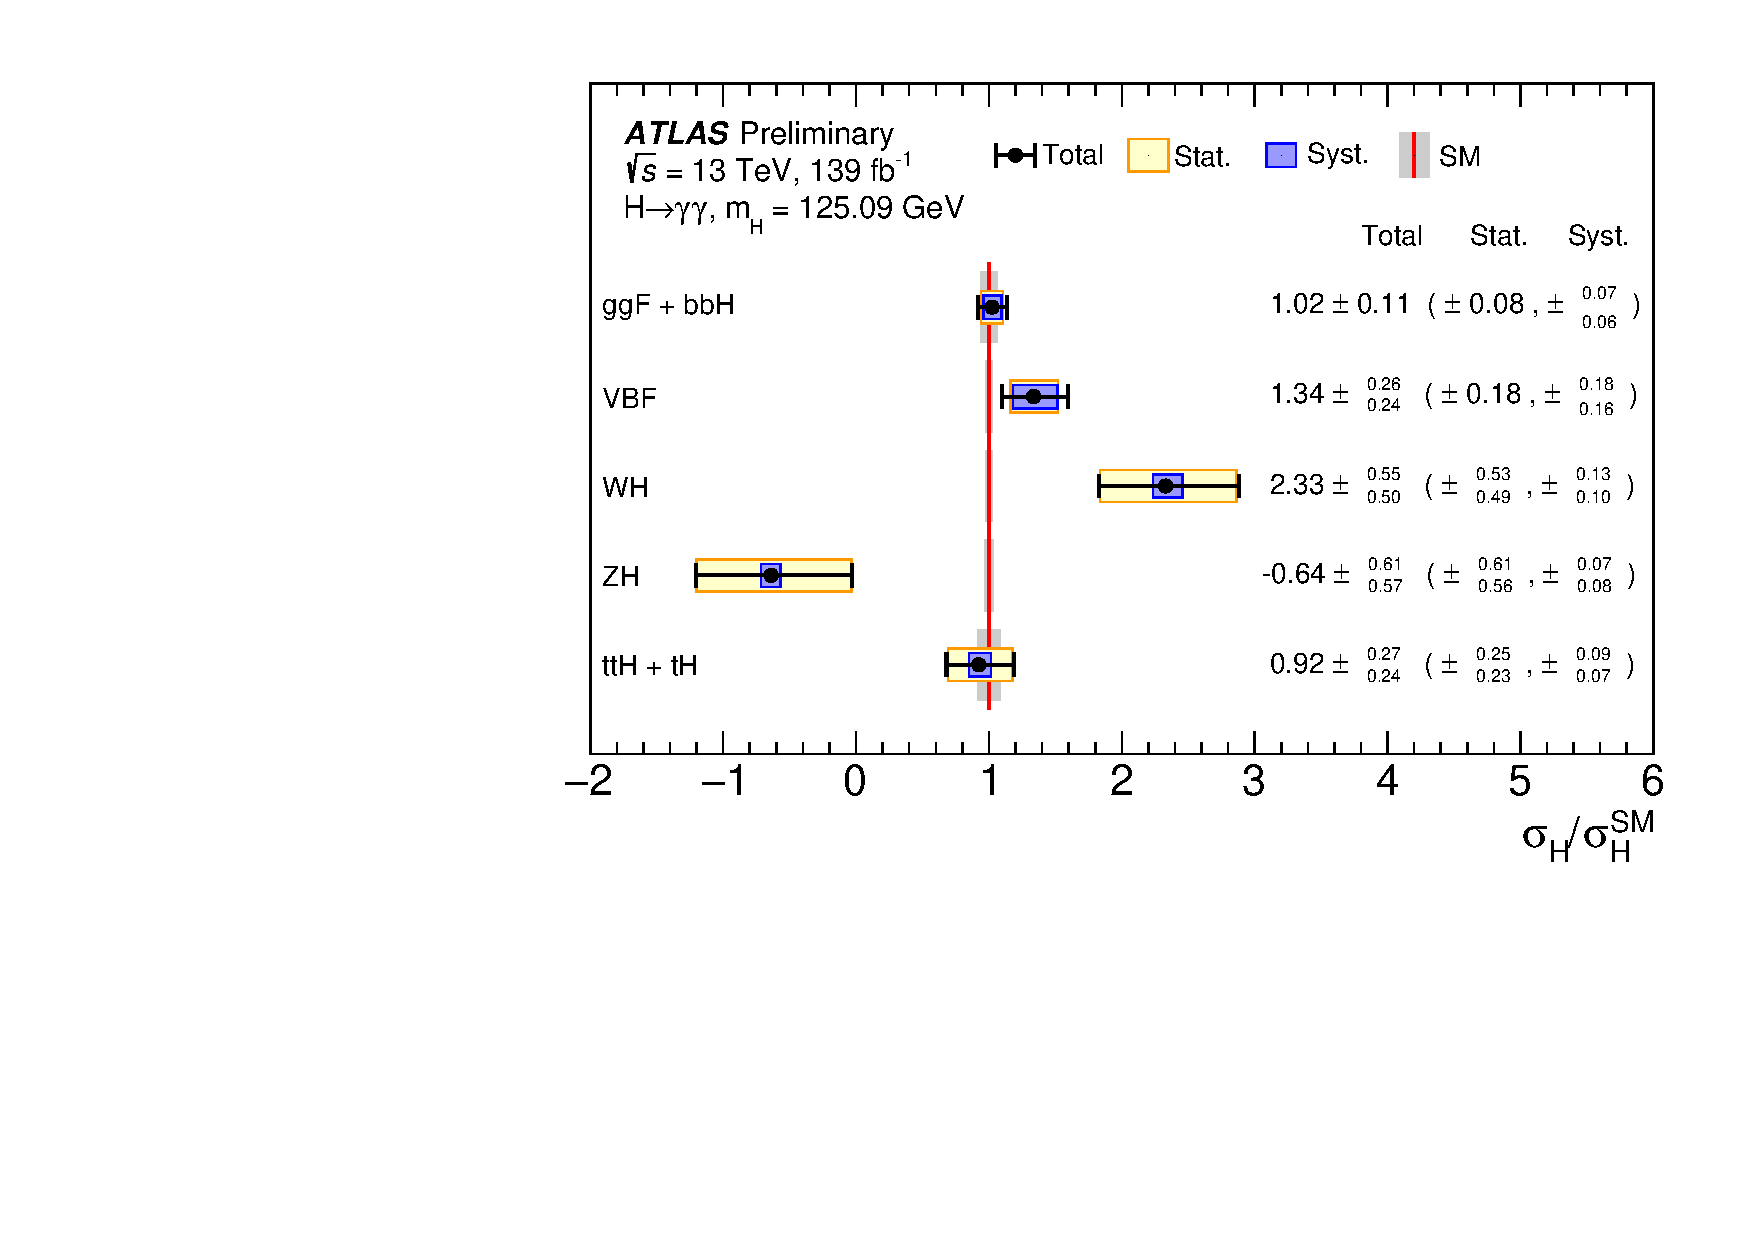
\includegraphics[width=0.9\textwidth]{figures/couplings_chapter/summary_5XS}
  \caption{Measured cross sections times branching fraction for \ggF+~\bbH, \VBF, \VH\ and \ttH+~\tH\ production. The values are obtained from a simultaneous fit to all categories. The black error bars, blue boxes and yellow boxes show the total, systematic, and statistical uncertainties, while the gray bands show the theory uncertainties. }
  \label{fig:results:prodXS}
\end{figure}

\begin{table}
\begin{center}
\renewcommand{\arraystretch}{1.3}
\begin{tabular}{|cr|crclclcl|cl|crcr}
\hline \hline
Process       & \multicolumn{1}{c}{Value} & \multicolumn{3}{c|}{Uncertainty [fb] } & \multicolumn{1}{c|}{SM pred.} \\
 & \multicolumn{1}{c}{[fb]}  & Total  & \small{Stat.}      & \small{Syst.}        & \multicolumn{1}{c|}{[fb]} \\
\hline
\ggF + \bbH &	104	& $^{+	11	}_{	-11	}$ & $^{+	8	}_{	-8	}$ & $^{+	7	}_{	-6	}$ & 	$102 \pm 5$	\\
\VBF        &	10.7	& $^{+	2.1	}_{	-1.9	}$ & $\pm 1.4$ & $^{+	1.4	}_{	-1.3	}$ & 	$8.0 \pm 0.2$	\\
\WH         &	6.4	& $^{+	1.5	}_{	-1.4	}$ & $^{+	1.5	}_{	-1.3	}$ & $^{+	0.4	}_{	-0.3	}$ & 	$2.7 \pm 0.1$ \\
\ZH         &	-1.2	& $^{+  1.1     }_{     -1.0    }$ & $^{+  1.1     }_{     -1.0    }$ & $\pm 0.1$ & 	$1.8~^{ +0.1}_{ -0.1}$ \\
\ttH+~\tH   &	1.2	& $^{+  0.4     }_{     -0.3    }$ & $\pm 0.3$ & $\pm 0.1$ & 	$1.3 \pm 0.1$	\\

\hline \hline
\end{tabular}
\end{center}
\caption{Best-fit values and uncertainties for $\sigma \times Br_{\gamma \gamma}$ in each of the five major production modes. The total uncertainties are decomposed into statistical and systematic components. Expected values are also shown for the cross-section of each process.}
\label{tab:results:prodXS}
\end{table}

\begin{figure}[tpb!]
\centering
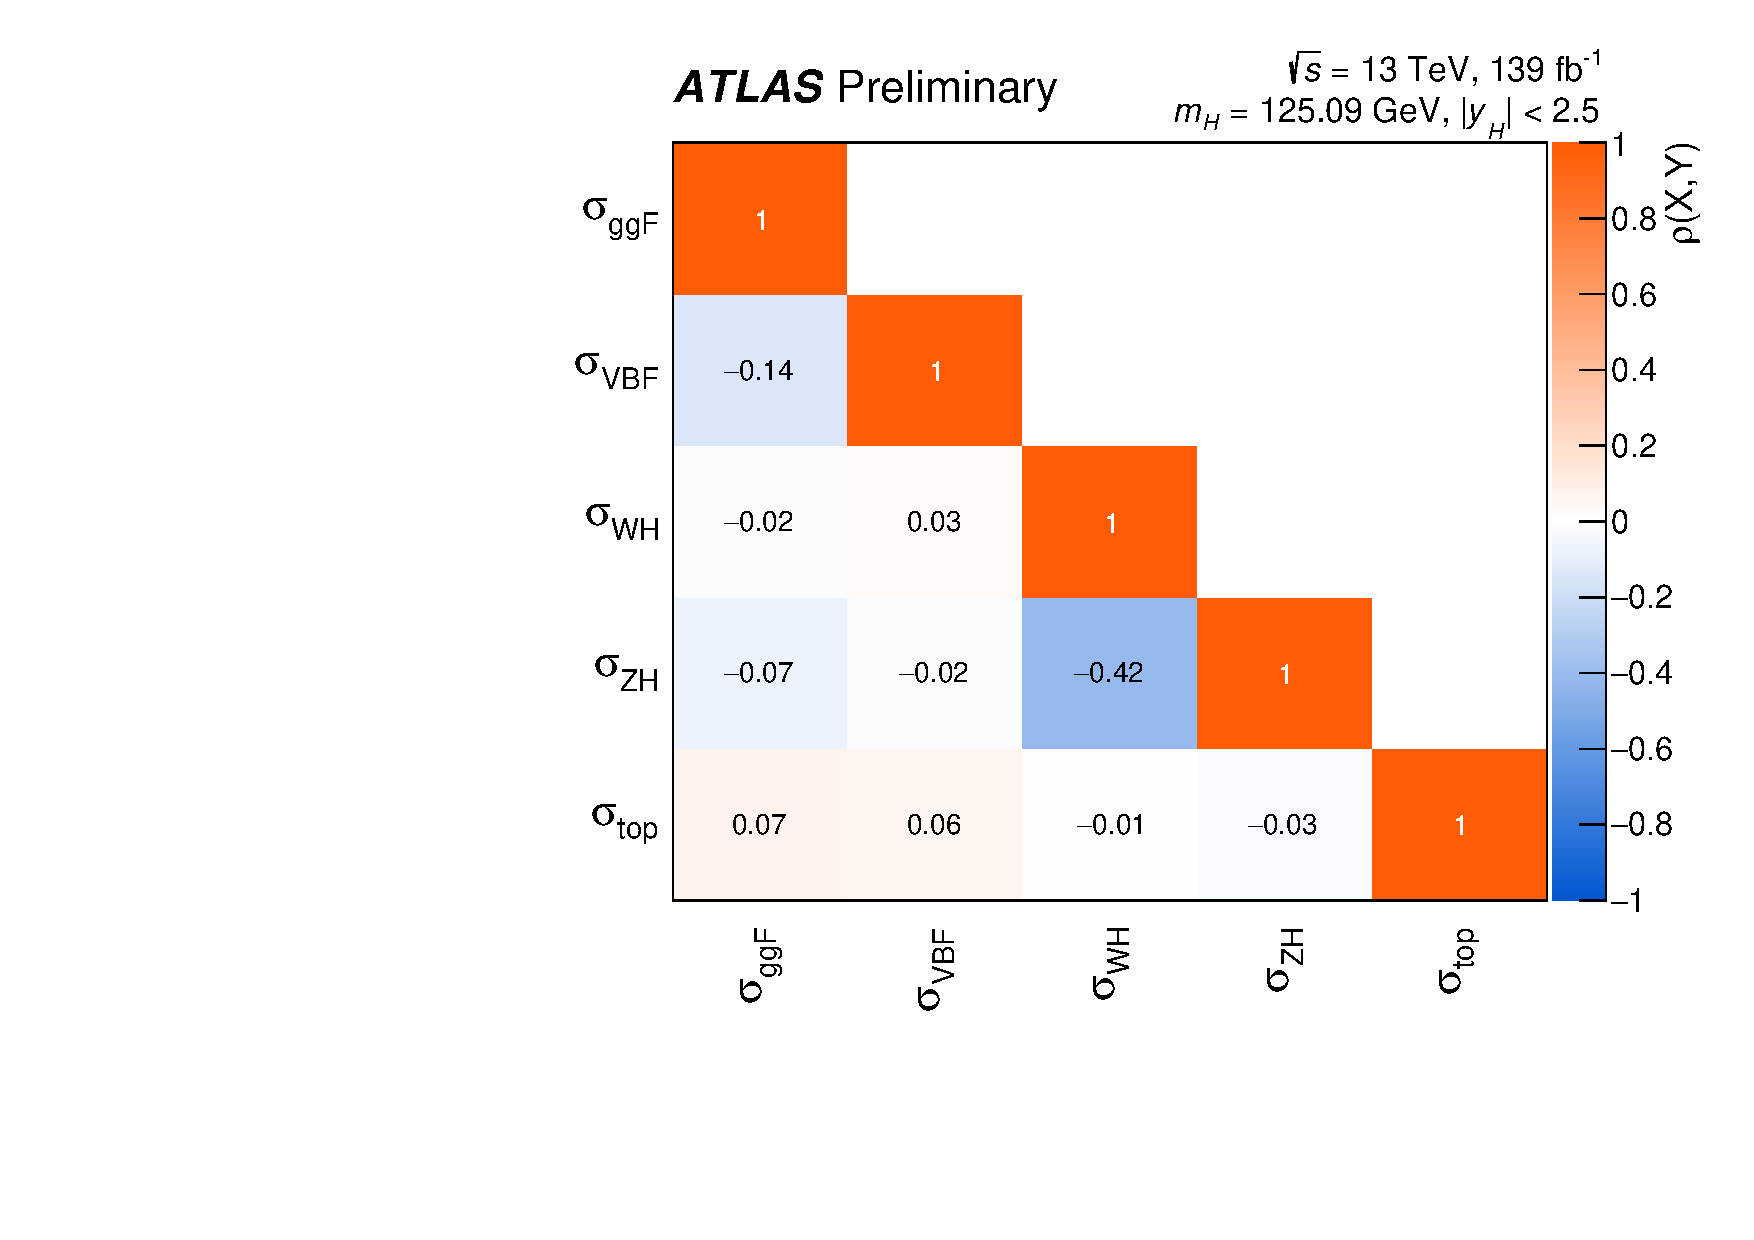
\includegraphics[width=.7\textwidth]{figures/couplings_chapter/corrmat_obs_5XS.pdf}
\caption{Correlation matrix for the five-production-mode fit.
}
\label{fig:results:prodXS_corr}
\end{figure}

\subsection{STXS} \label{sec:STXS}

In order to avoid large uncertainties and correlations (computed from SM expectation using post-fit Asimov), several of the 44 STXS truth bins are merged in a so-called "strong merging scheme" resulting in 27 truth bins being targeted. The merging is as follows:

\begin{itemize}
\item For $gg\rightarrow H$, the four bins in regions of $350 GeV < m_{jj} < 700 GeV$ and $m_{jj}> 700 GeV$ are merged into a single $m_{jj} > 350 GeV$ bin. The $p_{T}^{H} > 650 GeV$ bin is also merged with the $450 GeV < p_{T}^{H} < 650 GeV$ bin into a single $p_{T}^{H} > 450 GeV$ bin. The splits at $p_{T}^{Hjj}=25 GeV$ are removed.
\item For $qq' \rightarrow Hqq'$ processes, the 0-jet and 1-jet regions are combined, as are the regions corresponding to $m_{jj} < 60 GeV$ and $120 GeV < m_{jj} < 350 GeV$. The splits at $p_{T}^{Hjj}=25 GeV$ are removed, and a single  $p_{T}^{H} > 200 GeV$ region is also defined by merging together the two regions corresponding to $350 GeV < m_{jj}<700 GeV$ and $m_{jj}>700 GeV$.
\item In both the $qq \rightarrow WH$ and $pp \rightarrow ZH$ processes, only the two regions $p_{T}^{V} < 150 GeV$ and $p_{T}^{V} > 150 GeV$ are retained.
\item In the $ttH$ process, the $200 GeV < p_{T}^{H} < 300 GeV$ and $p_{T}^{H} > 300 GeV$ regions are combined into a single $p_{T}^{H} > 200 GeV$ region.
\item The $tWH$ and $tHjb$ regions are merged into a single $tH$ region.
\end{itemize}

As in the other schemes, $(\sigma \times Br_{\gamma \gamma})$ is measured for each of the 27 truth regions. Results are shown in Table \ref{tab:results:STXS} and Figure \ref{fig:results:STXS}. The correlation matrix is shown in Figure \ref{fig:results:STXS_corr}. All categories are statistically limited, and no substantial deviation from the Standard Model is observed.

\begin{table}[!htp]
  \begin{center}
  \small
   \renewcommand{\arraystretch}{1.35}
    \begin{tabular}{l|rlll@{ }|l@{ }}
      \hline \hline
      \multirow{2}{*}{STXS region $(\sigma_i \times Br_{\gamma\gamma})$} & \multicolumn{1}{c}{Value} & \multicolumn{3}{c|}{ Uncertainty [fb]} & \multicolumn{1}{c}{SM prediction} \\
                                                            &  \multicolumn{1}{c}{[fb]}                & Total   & Stat.                & Syst.   & \multicolumn{1}{c}{[fb]}   \\
\hline

\ggHjPt{0}{}{10}{}             & $11.4$   & $^{+ 4.7}_{-4.5}$  & $^{+3.9}_{-3.9}$  & $^{+2.7}_{-2.4}$  & $15.0  \pm 2.0$            \\
\ggHjPt{0}{10}{200}{}          & $54.7$  & $^{+ 9.4}_{-8.9}$  & $^{+7.0}_{-7.0}$  & $^{+6.1}_{-5.2}$  & $46.8   ^{+3.5}_{-3.6}$    \\
\ggHjPt{1}{0}{60}{}         & $13.4$      & $^{+ 6.5}_{-6.3}$  & $^{+5.9}_{-5.9}$  & $^{+2.8}_{-2.4}$  & $14.7  \pm 2.1$            \\
\ggHjPt{1}{60}{120}{}         & $12.1$    & $^{+ 4.0}_{-3.8}$  & $^{+3.8}_{-3.8}$  & $^{+1.5}_{-0.6}$  & $10.2  \pm 1.5$            \\
\ggHjPt{1}{120}{200}{}         & $1.2$   & $^{+ 0.9}_{-0.9}$  & $^{+0.9}_{-0.9}$  & $^{+0.2}_{-0.2}$  & $1.7  \pm 0.3$           \\
\ggHmPt{}{350}{}{60}{}     & $1.2$        & $^{+ 3.4}_{-3.2}$  & $^{+3.1}_{-3.0}$  & $^{+1.5}_{-1.0}$  & $2.6   \pm 0.6$            \\
\ggHmPt{}{350}{60}{120}{}     & $1.1$     & $^{+ 2.4}_{-2.4}$  & $^{+2.3}_{-2.3}$  & $^{+0.5}_{-0.5}$  & $4.1   \pm 0.9$            \\
\ggHmPt{}{350}{120}{200}{}     & $1.3$    & $^{+ 1.0}_{-1.0}$  & $^{+0.9}_{-0.9}$  & $^{+0.4}_{-0.3}$  & $2.1   \pm 0.6$            \\
\ggHmPt{350}{}{}{200}{}        & $4.5$    & $^{+ 2.0}_{-1.8}$  & $^{+1.8}_{-1.7}$  & $^{+0.9}_{-0.6}$  & $2.0  \pm 0.25 $          \\
\ggHPt{200}{300}{}             & $1.0$   & $^{+ 0.4}_{-0.4}$  & $^{+0.4}_{-0.4}$  & $^{+0.1}_{-0.1}$  & $1.04  \pm 0.3$           \\
\ggHPt{300}{450}{}             & $0.05$  & $^{+ 0.14}_{-0.12}$  & $^{+0.13}_{-0.12}$  & $^{+0.03}_{-0.02}$  & $0.24 \pm 0.08$          \\
\ggHPt{450}{}{}                & $0.07$  & $^{+ 0.06}_{-0.05}$  & $^{+0.06}_{-0.05}$  & $^{+0.01}_{-0.00}$  & $0.04 \pm 0.02$          \\
\Hqqj{01}{}                    & $7.4$   & $^{+ 5.9}_{-5.2}$  & $^{+5.5}_{-4.9}$  & $^{+2.1}_{-1.8}$  & $4.8  ^{+0.1}_{-0.1}$   \\
Hqqm{0}{60}{} +               & \multirow{2}{*}{$5.2$}      & \multirow{2}{*}{$^{+ 3.0}_{-2.8}$}  & \multirow{2}{*}{$^{+2.8}_{-2.7}$}  & \multirow{2}{*}{$^{+1.2}_{-0.9}$}  & \multirow{2}{*}{$1.65 \pm 0.05$}          \\ \Hqqm{120}{350}{}              & & & & & \\
\Hqqm{60}{120}{}               & $0.9$    & $^{+ 1.1}_{-1.0}$  & $^{+1.1}_{-1.0}$  & $^{+0.3}_{-0.3}$  & $1.20 \pm 0.04$          \\
\HqqmPt{350}{700}{}{200}{}     & $1.0$   & $^{+ 0.9}_{-0.8}$  & $^{+0.8}_{-0.7}$  & $^{+0.5}_{-0.4}$ & $1.24  \pm 0.04$         \\
\HqqmPt{700}{}{}{200}{}        & $1.8$   & $^{+ 0.6}_{-0.5}$  & $^{+0.5}_{-0.4}$  & $^{+0.4}_{-0.3}$  & $1.67  \pm 0.05$         \\
\HqqmPt{350}{}{200}{}{}        & $0.5$   & $^{+ 0.2}_{-0.2}$  & $^{+0.2}_{-0.1}$  & $^{+0.07}_{-0.06}$  & $0.36 \pm 0.01$          \\
\HlnPt{}{150}{}                & $1.8$   & $^{+ 0.5}_{-0.5}$  & $^{+0.5}_{-0.5}$  & $^{+0.2}_{-0.2}$  & $0.76  \pm 0.02$         \\
\HlnPt{150}{}{}                & $0.3$   & $^{+ 0.1}_{-0.1}$  & $^{+0.1}_{-0.1}$  & $^{+0.02}_{-0.02}$  & $0.124 \pm 0.005$        \\
\HllPt{}{150}{}                & $-0.5$  & $^{+ 0.4}_{-0.4}$  & $^{+0.4}_{-0.4}$  & $^{+0.1}_{-0.1}$  & $0.45 \pm 0.02$          \\
\HllPt{150}{}{}                & $-0.01$         & $^{+ 0.10}_{-0.09}$  & $^{+0.10}_{-0.08}$  & $^{+0.01}_{-0.02}$  & $0.092 \pm 0.011$          \\
\ttHPt{}{60}{}             & $0.2$       & $^{+ 0.2}_{-0.2}$  & $^{+0.2}_{-0.2}$  & $^{+0.06}_{-0.05}$  & $0.27 \pm 0.04$          \\
\ttHPt{60}{120}{}             & $0.3$    & $^{+ 0.2}_{-0.2}$  & $^{+0.2}_{-0.2}$  & $^{+0.04}_{-0.03}$  & $0.40 ^{+0.05}_{-0.04}$          \\
\ttHPt{120}{200}{}             & $0.3$   & $^{+ 0.2}_{-0.2}$  & $^{+0.2}_{-0.2}$  & $^{+0.05}_{-0.04}$  & $0.29 \pm 0.03$          \\
\ttHPt{200}{}{}                & $0.2$   & $^{+ 0.09}_{-0.08}$  & $^{+0.09}_{-0.08}$  & $^{+0.02}_{-0.02}$  & $0.18 \pm 0.02$          \\
\tH                            & $0.2$   & $^{+ 0.6}_{-0.5}$  & $^{+0.6}_{-0.4}$  & $^{+0.2}_{-0.2}$  & $0.19 ^{+0.01}_{-0.02}$ \\
\hline
    \end{tabular}
  \end{center}
  \caption{ Best-fit values and uncertainties for the cross-section times \Hyy\ branching ratio $(\sigma_i \times Br_{\gamma\gamma})$ in each STXS region. The total uncertainties are decomposed into statistical and systematic components. SM predictions are also shown for each quantity.}  
  \label{tab:results:STXS}
\end{table}

\begin{figure}[!tp]
  \centering
  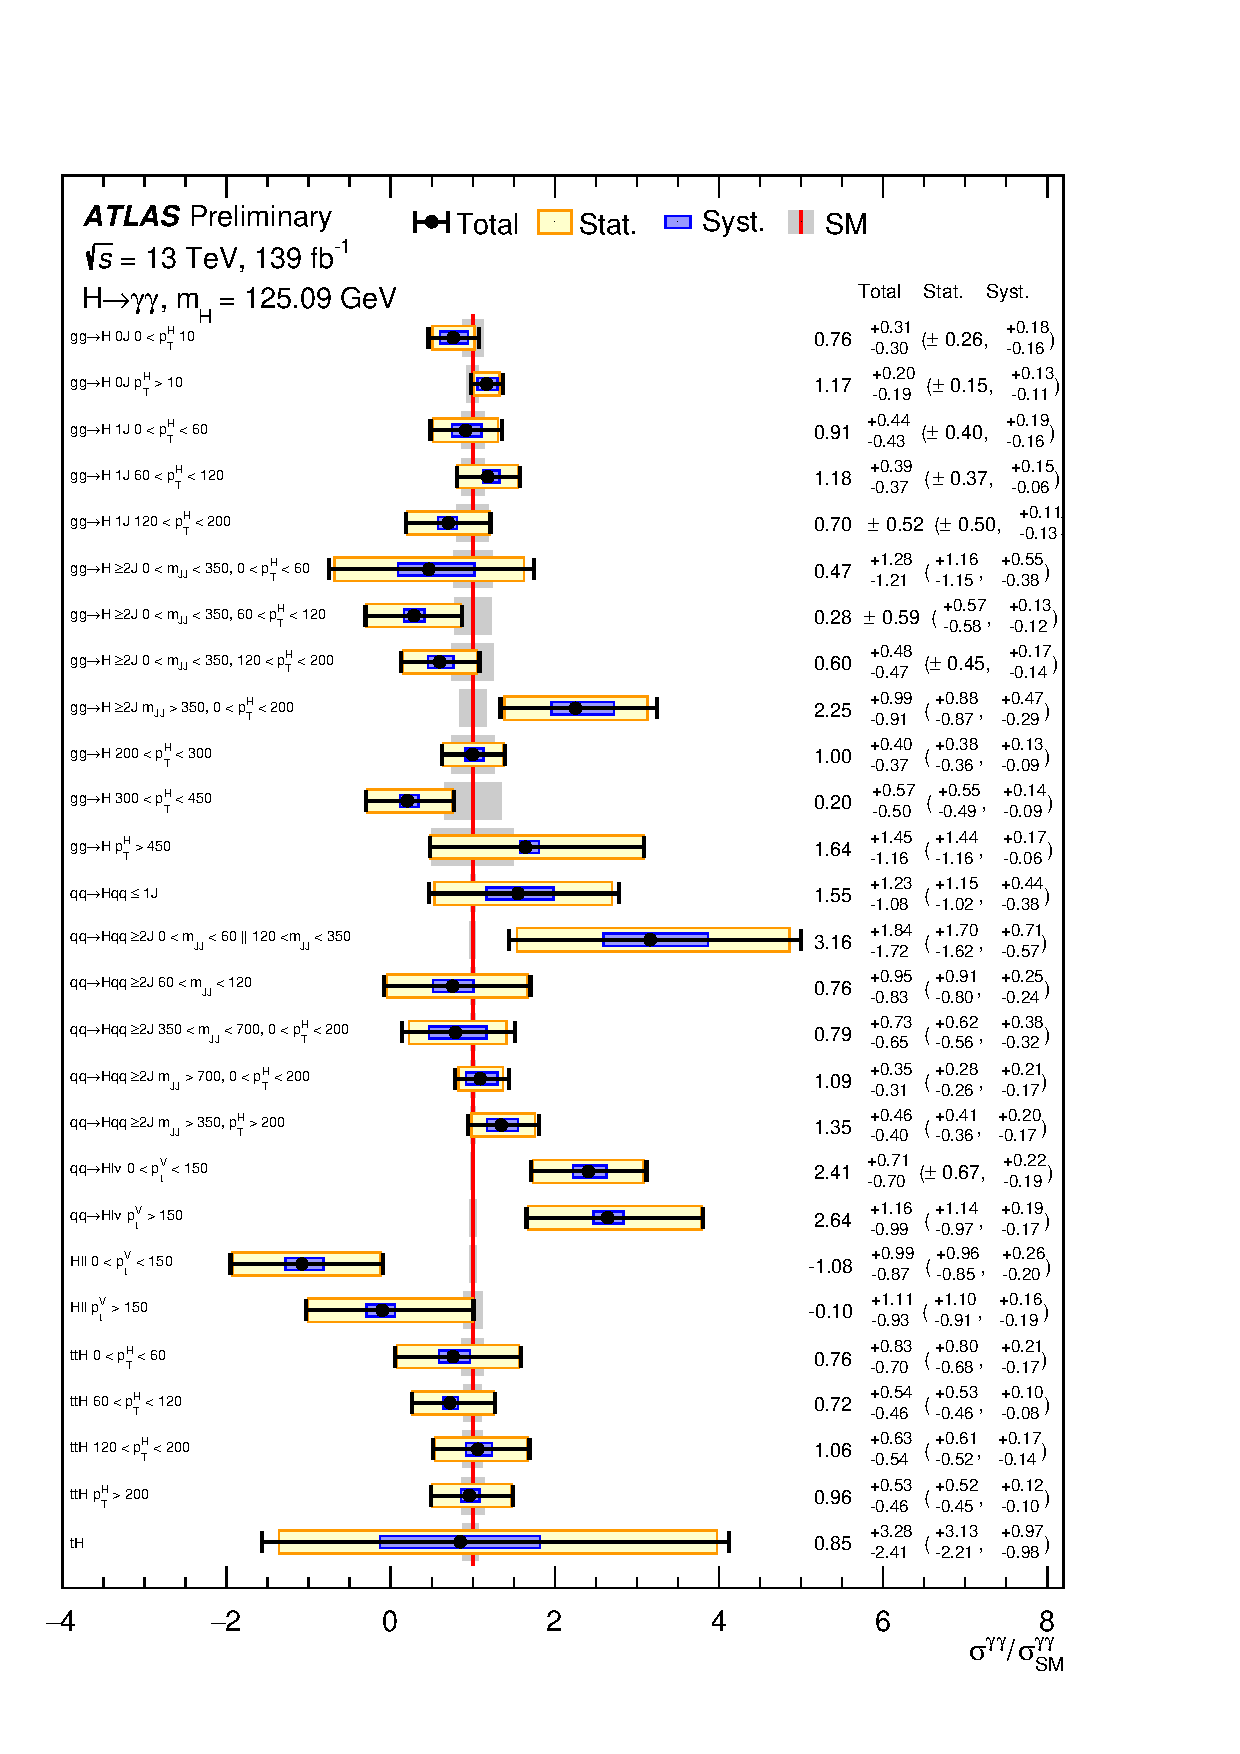
\includegraphics[width=.875\textwidth]{figures/couplings_chapter/summary_stxs.pdf}
  \vspace{-10pt}
  \caption{Measured cross sections times branching fraction for the cross sections in each analysis category. The black error bars, blue boxes and yellow boxes show the total, systematic, and statistical uncertainties, respectively, while the gray bands show the theory uncertainties.}
  \label{fig:results:STXS}
\end{figure}

\begin{figure}[!tpb]
\centering
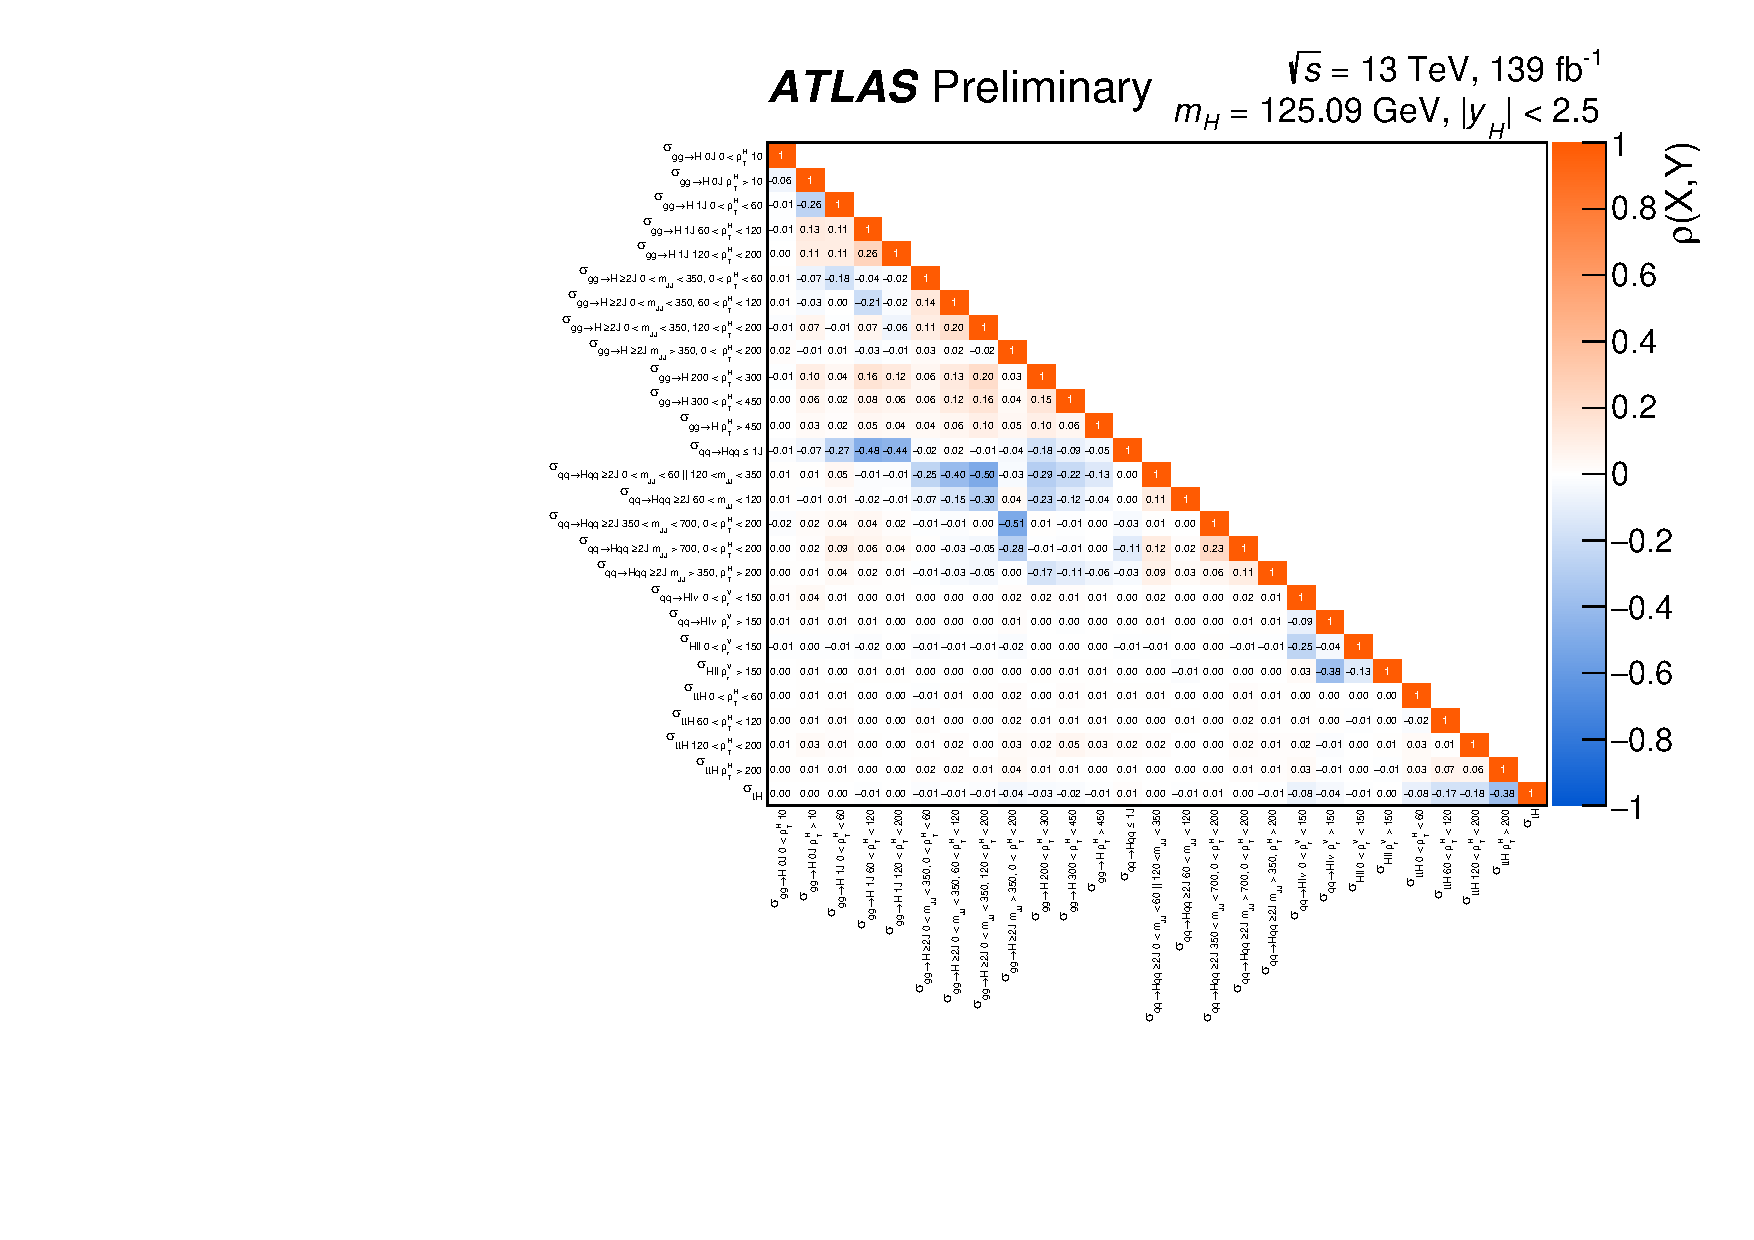
\includegraphics[width=.995\textwidth]{figures/couplings_chapter/corrmat_STXS_obs.pdf}
\caption{Correlation matrix for the STXS measurement.
}
\label{fig:results:STXS_corr}
\end{figure}



